%%%%%%%%%%%%%%%%%%%%%%%%%%%%%%%%%%%%%%%%%%%%%%%%%%%%%%%%%%%%%%%%%%%%%%%%%%%%%%%
% intro.tex: Introduction to the thesis
%%%%%%%%%%%%%%%%%%%%%%%%%%%%%%%%%%%%%%%%%%%%%%%%%%%%%%%%%%%%%%%%%%%%%%%%%%%%%%%%
\chapter{sCO2}
\label{sCO2_chapter}
%%%%%%%%%%%%%%%%%%%%%%%%%%%%%%%%%%%%%%%%%%%%%%%%%%%%%%%%%%%%%%%%%%%%%%%%%%%%%%%%


\section{Introduction}
%In the present electrification age, natural gas turbines play a vital role in power generation. Natural gas is expected to increase the total electricity supply from 3826 billion kWh in 2012 to 4954 billion kWh in 2040 \mbox{\citep{outlook2014early}}. The high emission of \mbox{\ce{CO2}} and \mbox{\ce{NOx}} in natural gas combustion severely limits its rapid development.
Semi-closed supercritical carbon dioxide (\ce{sCO2}) oxy-combustion is a promising candidate for the next generation power cycles, since it is one of the potential solutions to effectively remove \ce{CO2} and \ce{NO_x} emissions from power generation. %This gas turbine system uses 
In a semi-closed \ce{sCO2} cycle (see details in Appendix~\ref{app:sCO2cycle}), the heat input typically comes from oxy-fuel combustion using either natural gas or syngas from a coal gasification process~\citep{mcclung2015comparison}. This direct heating semi-closed \ce{sCO2} power cycle can allow higher turbine inlet temperature than the indirect heating closed \ce{sCO2} cycles to achieve higher efficiency. %, but also can deliver optimal performance at higher pressures. 
The \ce{NO_x} emission is directly avoided by oxy-combustion (i.e., using pure oxygen rather than air as the oxidizer). The combustion products (primarily \ce{CO2} and \ce{H2O}) can be recycled. %, and \ce{H2O} and excess \ce{CO2} are captured and removed from the system. 
%It is an important step towards ``zero carbon emission'' combustion and has been listed as one of the ten breakthrough technologies in 2018 by MIT Technology Review. %On the other hand, since the hot \ce{sCO2} holds on high energy density, when it is used as the working fluid instead of cold air or oxygen. Near the nozzle outlet, the \ce{sCO2} cycle can get higher overall efficiency with a smaller equipment size \citep{dostal2004supercritical}. 
In addition, since the high pressure \ce{sCO2} holds high energy density, it can reduce the equipment size and improve the power density relative to air or oxygen~\citep{dostal2004supercritical,ahn2015review}. % Because of these advantages, semi-closed \ce{sCO2} gas turbine power cycle is a strong candidate for the next generation of power cycles~\citep{dostal2004supercritical}.
%In the field of semi-closed \mbox{\ce{sCO2}} cycles, the Allam-Fetvedt cycle, commonly referred to the Allam cycle~\mbox{\cite{allam2013system}}, is a breakthrough invention, which has a high efficiency without any auxiliary physical/chemical absorption system. The Allam cycle is a highly recuperative cycle due to its internal recuperators and thermal integration between the power cycle and air separation unit.
%\textcolor{red}{The semi-closed sCO2 cycle, in which the heat input typically results from an oxy-fuel combustion using either natural gas or syngas from a coal gasification process, has obtained a lot of interests recently, because this direct heating sCO2 power cycle can not only allow higher cycle temperature than indirect sCO2 cycles but also deliver optimal performance at higher pressure ratios. Therefore, the working fluid can hold a higher power density compared to the indirect heating cycles. }
Although the advantages of the semi-closed \ce{sCO2} gas turbine cycles are evident, the design of these cycles with oxy-combustion thermal input requires extensive knowledge of the real-fluid thermodynamics of multicomponent mixtures at a broad range of temperature and pressure conditions.
%Specifically, researchers aim to tackle the following challenges: %introduced by this semi-close \ce{sCO2} cycle as well as the more ambitious operating conditions, namely 
%the impurities in \ce{CO2} due to the combustion, including fuel, oxygen, and water; the compressor blade erosion at high and low temperatures; and the thermoacoustic combustion instability at high-pressure ambient conditions \cite{banuti2018large,abdul2017cfd,barak2020ignition}.

%The aim of this study is to discuss the effects of the impurities in the working fluid on the system performance. In order to investigate this, a robust VLE calculator for multicomponent is necessary.

%Although the advantages of semi-closed \ce{sCO2} gas turbine cycles are evident, there are only very limited works on the real-fluid thermodynamics involved in such systems.
%However, the real-fluid thermodynamics and combustion of natural gas in supercritical carbon dioxide (\ce{sCO2}) diluent conditions lack investigation. 
%The design of \ce{sCO2} gas turbine systems with oxy-combustion thermal input requires extensive knowledge of the real-fluid thermodynamics of multicomponent mixtures at a broad range of temperature and pressure conditions. %The limited knowledge presents a formidable challenge to the design of the next generation \ce{sCO2} gas turbine systems.
%The existing studies about the \ce{sCO2} gas turbine systems mainly focused on the \ce{sCO2} Brayton cycle and low \ce{CO2} concentration combustion at low or moderate pressure conditions in shock tubes~\citep{shao2018shock}. Koroglu et al.~\citep{koroglu2016shock} conducted a shock tube experiment to study the combustion behaviors of \ce{CH4}/\ce{CO2}/\ce{O2} mixtures at 1577–2144 K, but only at 0.53–4.4 bar. The equivalence ratio was in the range of 0.5–2.0, and the \ce{CO2} concentration was 0, 30, 60\%. Recently, Shao et al.~\citep{shao2019ignition} extended the earlier studies to significantly higher pressures of 27–311 bar. Their \ce{CO2} concentration was above 85\%, and the ignition characteristics were provided. However, they did not cover the overall \ce{sCO2} gas turbine performance but only focused on ignition. %The above experimental results have shown that the combustion reactions behave differently with variation in the proportion of nitrogen and carbon dioxide \citep{hu2014investigation}.

%Motivated by semi-closed \ce{sCO2} cycles, this work will investigate the multicomponent effects of supercritical \ce{CO2} system with \ce{H2O} addition. 

%\subsection{Motivations: effects of mixture critical point and phase separation on the \ce{sCO2} gas turbine systems}
In the semi-closed \ce{sCO2} cycles, impurities in \ce{CO2} due to the combustion make it different from the traditional closed \ce{sCO2} cycles, and the semi-closed \ce{sCO2} cycles are no more single-component systems \cite{abdul2017cfd,barak2020ignition}.
%In semi-closed \ce{sCO2} cycles, since combustion occurs inside the system, fuel, oxidizer, and products are mixed with the working fluid. Different from traditional closed \ce{sCO2} cycles, semi-close \ce{sCO2} cycles are no more single component systems. %(see more details about the comparison between the two types of cycles in \ref{app:sCO2cycle:TwoCycleComp}). 
The impurities, especially components with high critical pressure such as \ce{H2O}, could significantly change the mixture critical point and phase boundary, and consequently, affect the thermodynamic proprieties of the working fluid. Hence, the thermodynamic characteristics of the mixture may deviate a lot from a single component. These effects may trigger phase separation, which may affect the system performance (e.g., thermal efficiency) and/or may cause safety issues. Thus, multicomponent effects on the \ce{sCO2} systems (in terms of the effects of mixture critical point and phase separation) are important and need to be investigated.

\textbf{Effects of mixture critical point:}
%Supercritical region can be divided into liquid-like and gas-like regions, and the boundary between the two regions is the Widom line. The properties of supercritical fluid across over the Widom line show a sudden change~\cite{banuti2020between}. Supercritical liquid-like fluid has low compressibility to reduce the compression work necessary for a given pressure ratio \citep{ahn2015review,invernizzi2017prospects}, which can significantly improve the thermal efficiency of the whole system. In addition, the 
Supercritical fluid, such as \ce{sCO2}, holds high energy density $\rho e$ near its mixture critical point due to the large variation of density $\rho$, which results in a large change in specific heat capacity $c_p$ for a small temperature change. Therefore, it is better to keep the fluid temperature and pressure close to the mixture critical point to take this special advantage of high energy density to compact the turbomachinery. Accordingly, when designing and analyzing a semi-closed \ce{sCO2} system, an accurate determination of the mixture critical point of a multicomponent mixture becomes very important.% to achieve high thermal efficiency.

%Supercritical region can be divided into liquid-like and gas-like regions, and the boundary between two regions is the Widom line. Based on Banuti et al.~\cite{banuti2020between}, the properties of supercritical fluid across over the Widom line show a sudden change, which can significantly affect the estimated thermal efficiency of the whole system. In addition, steep property gradients and response function extrema present at the near-critical pressure and temperature, and the transition region has a finite width and widens towards higher pressures. Therefore, the determination of the critical point is very important. For pure \ce{CO2} in traditional closed \ce{sCO2} cycle, its critical point is known. However, with respect to the mixtures in semi-closed \ce{sCO2} gas turbine cycle, some impurities will be mixed into the working fluid in addition to \ce{CO2} due to the direct combustion. Then the critical points will depend on the mixture compositions, and the thermodynamic characteristics of the mixture may deviate a lot from a pure component. Whether the mixture critical points of the fluids in semi-closed \ce{sCO2} gas turbine cycle can affect the performance of system remains unclear up to now.
%\textcolor{red}{For the typical closed \ce{sCO2} system, the working fluid is pure \ce{sCO2}, while in the practical semi-closed \ce{sCO2} applications (i.e., the focus of this study), some impurities will be mixed into the working fluid in addition to \ce{CO2} due to the direct combustion. The true mixture critical point and properties of the working fluid, as well as the related effects on the system performance needs to be further evaluated.}
%\textcolor{red}{Specifically, as semi-closed \ce{sCO2} system, it needs to face the problem of the \ce{CO2} impurities, which makes it unclear whether the working fluids remain in a single-phase throughout the whole \ce{sCO2} gas turbine cycle. One aim of this study is to discuss the effects of the impurities in the working fluid on the system performance}
%Since the high concentration of \ce{sCO2} is beneficial for clean combustion, a large amount of carbon dioxide needs to be captured. %and a possible higher turbine inlet temperature needs to be handled. 
%Therefore, the cooler and remover are added in the downstream of compressor rather than the upstream like the typical gas turbine or traditional \ce{sCO2} cycles.
\textbf{Effects of phase separation:}
%Phase separation caused by multicomponent effects is also important.
%Baltadjiev et al.~\cite{baltadjiev2015investigation} and Brinckman et al.~\cite{brinckman2019numerical} suggested that due to the local flow acceleration, nucleation is likely to occur at the leading edge of the impeller as the critical point is approached. The droplets generated by nucleation could cause erosion of the impeller. 
In the compressor of a semi-closed \ce{sCO2} cycle, phase boundary change caused by multicomponent effects is a potential cause of phase separation. It may lead to compressor blade erosion, which has been widely investigated in traditional steam turbines \cite{ahmad2009experimental} but not in \ce{sCO2} gas turbines. % (see more details in \ref{app:sCO2cycle:compressor}). 
In the \ce{sCO2} oxy-combustor (i.e., the reactor in Fig.~\ref{fig1} of Appendix~\ref{app:sCO2cycle}), phase separation caused by multicomponent effects may also occur due to the mixing between the working fluid (\ce{CO2}/\ce{H2O}) and injected \ce{O2} and \ce{CH4}. For the pure gas phase, the mass mixing time scale is very small due to the large mass diffusivity, and the corresponding ``effective'' ignition delay is also short. For a two-phase state, due to the presence of the liquid phase, the mass diffusivity is decreased, which increases the mass mixing time, but the thermal diffusivity is increased, which reduces the thermal conduction time. In these ways, multicomponent effects may affect the cold ignition in terms of ``effective'' ignition delay. In addition, phase separation may lead to combustion-induced Rapid Phase Transition (cRPT)~\citep{basco2013effect}, which causes anomalous high or oscillating pressures to damage the equipment and cause safety issues.% (see more details in \ref{app:sCO2cycle:combustor}).

%\subsection{Objectives and outline of this study}
As mentioned above, multicomponent effects are important to understand the semi-closed \ce{sCO2} gas turbine performance, such as thermal efficiency, compressor blade erosion, and ``effective'' ignition delays. However, very few researchers have investigated the influence of impurities (e.g., \ce{H2O}, \ce{CH4}, and \ce{O2}) on the \ce{sCO2} systems \cite{vesely2019effect,pint2018effect}. 
To fill this scientific knowledge gap, the current fundamental study will focus on the multicomponent effects caused by impurities on the \ce{sCO2} systems. % on these effects and raise potential problems.
But please note that the simulation and optimization of the real \ce{sCO2} gas turbine systems (i.e., applied research) is out of the scope of this fundamental research and hence will not be covered in this paper.

%In this work, thermodynamic analysis is first carried out for the multicomponent \ce{CO2}/\ce{H2O} mixture relevant to \ce{sCO2} compressors under a broad range of temperature and pressure conditions, which provides valuable information for the thermal efficiency of \ce{sCO2} compressors. Within the same framework, thermodynamic analysis is also conducted for the mixture of \ce{CH4}/\ce{CO2}/\ce{O2} with and without \ce{H2O} addition relevant to \ce{sCO2} oxy-combustors, and for the mixing process between the cold \ce{CH4} and the hot working fluid (either pure \ce{CO2} or \ce{CO2}/\ce{H2O} mixture).
%to understand its influence on the ``effective'' ignition delay. 
%In this work, thermodynamic analyses are first carried out for the mixture of \ce{CH4}/\ce{CO2} with and without \ce{H2O}, and for the mixing process between the cold \ce{CH4} and the hot working fluid (either pure \ce{CO2} or \ce{CO2}/\ce{H2O} mixture).
%Jet-in-crossflow computational fluid dynamics (CFD) simulations are then conducted to understand the mixing and phase separation processes in the \ce{sCO2} systems.%relevant to \ce{sCO2} oxy-combustors.
%In this study, the multicomponent effects on the supercritical \ce{CO2} (\ce{sCO2}) systems are investigated.

Around the year of 2000, many important works have been done to simulation high-pressure supercritical fluids \cite{oefelein2005thermophysical,bellan2000supercritical,yang2000modeling}. These works majorly used ``dense fluid'' methods to describe the thermodynamic properties in the supercritical region. However, it cannot capture the phase change and multiphase effects (e.g., two-phase thermodynamic and transport properties) near the critical point.
In order to investigate the multiphase thermodynamics of the \ce{sCO2} systems, a vapor-liquid equilibrium (VLE) model~\cite{michelsen1982isothermal,michelsen1987multiphase} is used in this study. The VLE model is based on the fundamental thermodynamics theory: Gibbs free energy is at a minimum at equilibrium. Hence, compared to low-pressure vaporization model, the VLE model is more suitable to capture phase boundary near the critical point. In this work, two VLE solvers (i.e., the isothermal-isobaric (TPn) flash solver~\cite{michelsen1982isothermal} and isobaric-isenthalpic (HPn) flash solver~\cite{michelsen1987multiphase}) are implemented, validated, and verified to predict the phase boundary and real mixture critical point, and simultaneously model the subcritical regime (with the consideration of phase change), the supercritical regime, as well as the transition between them. Thermodynamic and transport properties are evaluated based on the VLE solution, and thermodynamic relation are used to derive the formulas. %(i.e., the transcritical regime). 
%In CFD simulations, the VLE model assumes that phase separation is relaxed to equilibrium ``immediately". In other words, every point in the computational domain can be considered as in a local phase equilibrium state. 

VLE model have been used for thermal analysis of various mixture systems. Xu et al. investigated high-pressure VLE at 293 K for \ce{N2}/\ce{CH4}/\ce{CO2} systems \cite{xu1992high}. Perakis et al. modeled the VLE of the \ce{H2O}/ethanol/\ce{CO2} system \cite{perakis2006thermodynamic}. Pappa et al. modeled the VLE of the \ce{CO2}/\ce{H2O} system \cite{pappa2009thermodynamic}. Silvia et al. analyzed the \ce{CO2}-based mixture, and improved accuracy by using an advanced mixing rule \cite{lasala2016vle}. Legoix et al. investigated the mixtures of \ce{CH4}/\ce{CO2} and \ce{CH4}/\ce{CO2}/\ce{H2O} \cite{legoix2017phase}.    
Although some \ce{CO2}-containing mixtures have been studied using VLE theory, before the present work, detailed VLE thermodynamics analysis of semi-closed \ce{sCO2} systems has never been conducted in the literature, but such analysis is needed to better understand the \ce{sCO2} system performance (e.g., thermal efficiency) and predict potential phase change which may affect ignition or cause safety issues.

Although the VLE theory has been proposed for a long while~\cite{hanks1971calculation} and 0D VLE calculation can be done by publicly available software such as the National Institute of Standards and Technology (NIST) REFPROP code~\cite{lemmon2018nist}, the development of VLE-based computational fluid dynamics (CFD) solvers to capture high-pressure phase change interacting with flow field just started during the past decade. Matheis and Hickel~\cite{matheis2018multi} integrated VLE models to a 3D compressible solver to reveal special breakup behaviors at supercritical conditions, which was also reported in Roy and Segal's experimental results~\citep{roy2010experimental} and Ana et al.'s simulation work~\citep{star2006numerical}. %Moreover, the VLE model is also used to investigate the physics at high pressures. 
Yao et al. used the tangent plane distance (TPD) method, a phase stability test method in VLE theory, to investigate the effect of mass diffusion model on phase stability \citep{yao2019molecular}. Ray et al. used the 2D compressible governing equation in the spherical coordinate system to describe droplet fluid dynamics, and integrated a VLE model to investigate the droplet evaporation at high pressures \cite{ray2019two}. Yi et al. developed a compressible four-equation model for multicomponent two-phase flow coupled with VLE solvers. Ma et al. integrated their non-conservative double-flux model~\cite{ma2017entropy} to a CFD solver, developed an adaptive scheme by coupling existing quasi-conservative and fully-conservative scheme, and analyzed the mixing behavior of fully conservative and quasi-conservative schemes \citep{ma2019numerical}. Tudisco and Menon developed the formula to handle VLE in multi-component mixtures (i.e., more than two components), and combined the non-conservative double-flux model~\cite{ma2017entropy} to a CFD solver to investigate the VLE effects on mixing flows \cite{tudisco2020numerical}. In addition, Tudisco and Menon~\cite{tudisco2020vapor} also developed a p$\rho$n VLE solver, and investigated the coupling between thermodynamic and transport properties and governing equations. Different from all the works above, this research integrated VLE solver with a CFD solver based on the PIMPLE algorithm~\cite{holzmann2016mathematics}, which is a pressure-based scheme and suitable for ``low-Mach'' CFD simulation (but can also handle up to Mach 2 flows in its new transonic version). This work also developed a novel VLE-based tabulation method to make the VLE-based CFD solver computationally more affordable. 

%~\citep{banuti2017phase,matheis2018multi,yao2019molecular,tudisco2020numerical,tudisco2020vapor,ray2019two,ma2018numerical}.
%VLE model was also used in several previous works to simulate high-pressure fluid flows \citep{yao2019molecular,tudisco2020numerical,ray2019two}.
%\citet{yao2019molecular} to investigate the impact of diffusion models of a laminar counterflow flame at trans- and supercritical conditions. In \citet{ray2019two}'s, VLE theory is used to understand fuel droplets evaporation at high pressures. %The present framework has already been used in several previous works \citep{matheis2018multi} \citep{yi2019multicomponent}. 
%In the reactor, locally, the physical process involves mass/thermal diffusion and phase change.
%Mo and Qiao's molecular dynamics (MD) simulation results \cite{mo2017molecular} showed that when subcritical flow enters the supercritical regime, it only needs about 1 ns for surface tension to vanish, which indicates that phase equilibrium is reached ``immediately'' with respect to a typical time step size, and the phase change is dominated by slower diffusion processes. 
This work develops a VLE-based CFD simulation framework by coupling a pressure-based CFD solver with the HPn flash solver to capture the phase separation in high-pressure multiphase flows. The thermodynamics analyses (of multicomponent mixtures) and CFD simulations (of a laminar premixed shock tube and turbulent jet-in-crossflows) are then conducted to reveal several mechanisms of phase separation in the \ce{sCO2} systems.
%In this work, VLE solvers are implemented to capture the phase separation. 
%Peng-Robinson (PR) cubic equation of state (EOS) equipped with the VLE solver is used to predict real mixture critical points and thermal/transport properties. When coupling VLE with a computational fluid dynamics (CFD) solver, a tabulation method is used to avoid a large amount of on-the-fly VLE calculation which is computationally expensive.

The objectives of this research are:

\noindent$\bullet$ Understanding and quantifying the effects of combustion-relevant impurities (e.g., \ce{H2O}, \ce{CH4}, and \ce{O2}) on the mixture critical points and phase separation in the \ce{sCO2} systems. %relevant to the \ce{sCO2} gas turbine systems.

%\noindent$\bullet$ Discussing the thermodynamic and transport properties of the working fluid near the mixture critical point to understand the potential distinct performance of the semi-closed \ce{sCO2} cycles relative to the closed \ce{sCO2} cycles.
\noindent$\bullet$ Understanding and quantifying the effects of phase separation on different thermodynamic properties in the \ce{sCO2} systems.
%\noindent$\bullet$ Understanding the influence of phase separation on thermodynamic properties in \ce{sCO2} gas turbine systems.

\noindent$\bullet$ Understanding the mechanisms of phase separation in premixed \ce{sCO2} systems, particularly whether compression or expansion waves can trigger phase separation.

\noindent$\bullet$ Understanding the mechanisms of phase separation in non-premixed \ce{sCO2} systems, particularly whether flow field and mixing processes can trigger phase separation.
%\noindent$\bullet$ Discussing conditions under which phase separation could occur based on Jet-in-crossflow CFD simulations.
%\noindent$\bullet$ Predicting the potential phase separation at conditions relevant to the compressors and combustors of \ce{sCO2} gas turbine systems.%, and discussing its potential influence on thermodynamic properties and operation.

%\noindent$\bullet$ Discussing the potential influences of phase separation on thermodynamic properties and operation safety.

The paper is structured as follows. Section~\ref{sec:model} provides details of the numerical modeling, including the thermodynamics and transport models in Sec.~\ref{thermo models} and the CFD framework in Sec.~\ref{sec:model:cfd}. Section~\ref{sec:result} presents the results and discussion. Specifically, Section~\ref{sec:results:ThermAnalysis} presents the 0D analyses of the \ce{sCO2} systems, including the influence of impurities on premixed \ce{sCO2} systems in Sec.~\ref{sec:results:combustor:H2O}, the influence of mixture critical point and phase change on the thermodynamic properties in Sec.~\ref{sec:results:combustor:phase}, and the isobaric and isenthalpic (HPn) mixing process in Sec.~\ref{sec:results:combustor:HPn}. Section~\ref{sec:results:ShockTube} presents the 1D CFD simulation results of a laminar premixed \ce{sCO2} shock tube. Section~\ref{sec:results:JICF} presents the 3D large-eddy simulation (LES) results of turbulent jet-in-crossflows in the \ce{sCO2} systems.
%at conditions relevant to \ce{sCO2} compressors and turbines in Sec.~\ref{sec:result:compressor} and at conditions relevant to \ce{sCO2} oxy-combustors in Sec.~\ref{sec:result:combustor}.
Conclusions are summarized in Sec.~\ref{sec:conclusion}.

\section{Numerical Modeling}\label{sec:model}
\subsection{Models of thermodynamics and transport properties} \label{thermo models}
%In this work, 
\textbf{Models of thermodynamics:}
%There are two curves relevant to phase separation in thermodynamics -- the spinodal curve and the binodal curve. The spinodal curve is the boundary of the mechanically unstable region, which is used in Castiglioni and Bellan's work~\citep{castiglioni2018models}. Mechanical instability leads to a kind of phase separation, which is called spinodal decomposition. The binodal curve is the boundary of the chemically unstable region, which also includes the mechanically unstable region. Phase separation that occurs in the chemically unstable region is nucleation. Different from the spinodal decomposition, nucleation needs to overcome the energy barrier caused by surface tension \cite{ma2019numerical}. To model the process of nucleation and spinodal decomposition requires a more complicated model, which is out of scope of this study. 

This research investigated the systems of \ce{CO2/H2O/CH4/O2} mixtures. A conceptual schematic P-T diagram for the relevant  multicomponent system in this study is shown in Fig.~\ref{TPdiagram}, which is relatively simple comparing to many other mixtures. The whole region is divided into liquid, gas, two-phase, and supercritical regions. %The supercritical region can be further divided into liquid-like and gas-like supercritical regions, and there are several lines proposed to delimit two regions, including Fisher–Widom line \cite{fisher1969decay}, the Widom line\cite{xu2005relation}, and the Frenkel line \cite{brazhkin2012two}. 
In liquid, gas, and supercritical regions, only one phase is in the system. Peng-Robinson (PR)~\citep{peng1976new} cubic equation of state (EOS) and JANAF polynomials are used to evaluate thermodynamic properties. In the two-phase region, the vapor-liquid equilibrium (VLE) theory~\cite{hanks1971calculation} is need to determine phase fraction (i.e., the mole fraction of the gas phase) and compositions in the two phases, and then each phase uses the same model as above to evaluate thermodynamic properties. The mixture molar enthalpy and mixture compressibility factor are evaluated by blending (i.e., averaging weighted by phase fraction). Other thermodynamic properties are derived from relations between thermodynamic properties. Tudisco and Menon's work clearly discussed the relationship between properties and the associated calculation methods \cite{tudisco2020analytical}, which are used in this work. Whether a system is in the two-phase region is also determined by VLE theory: If the gas mole fraction obtained by VLE theory is between 0 and 1, then the system falls into the two-phase region, and the equilibrium between vapor and liquid should be observed.
%In this study, phase separation (i.e., nucleation and spinodal decomposition) is assumed to be relaxed to equilibrium ``immediately'', and the equilibrium state is described by the vapor-liquid equilibrium (VLE) theory. In this theory, phase boundary refers to the binodal curve (i.e., the dew curve and bubble curve connecting at the mixture critical point). %To obtain the equilibrium state in VLE theory, VLE solvers are implemented.
%Specifically, VLE solvers are used to determine the mixture critical point of the multicomponent mixture and to capture the phase separation. % in \ce{CO2} gas turbine systems. %VLE describes the phase equilibrium between liquid and vapor phases. 
%Solving the set of VLE equations gives the phase fraction and compositions in the two phases. 
%If the gas mole fraction %(i.e., the mole fraction of the vapor phase) 
%is equal to 1 or 0, then the system is in a purely gas or liquid phase, respectively. If the system falls into the two-phase region, the gas mole fraction is between 0 and 1, and the equilibrium between vapor and liquid should be observed. %If at certain conditions, thermodynamic properties become identical between liquid and gas, it indicates the occurrence of transcritical transition from a subcritical state to a supercritical state (which could be a liquid-like or gas-like state). 

Two VLE solvers are implemented to solve the VLE problem numerically: the isothermal and isobaric (TPn) flash \citep{michelsen1982isothermal} and isobaric and isenthalpic (HPn) flash \citep{michelsen1987multiphase}.
TPn flash is the basic VLE solver, which solves the set of VLE equations at a given temperature (T), pressure (P), and mole fraction of each component (n) in the system. TPn flash is used for thermodynamic analysis and is also used for building other VLE solvers such as the HPn flash. HPn flash solves the VLE equation set at given enthalpy (H) rather than temperature. More details about these two VLE solvers can be found in Michelsen's works~\cite{michelsen1982isothermal,michelsen1987multiphase} and the Supplementary Material. Tangent plane distance (TPD) method~\cite{michelsen1982isothermalP1} is used to ensure the correct convergence to the true VLE solution.  %Appendix~\ref{app:VLE}. 
The validation and verification of the VLE solvers are attached in Appendix~\ref{App:vali}.

In semi-closed \ce{sCO2} oxy-combustors, multiple fluids with different temperatures are mixed. There is almost no heat transfer to (or from) the surroundings, and except for pressure work, there is no other work done on (or by) the surroundings. Hence, the mixing of multiple fluids is isenthalpic~\cite{serrano2018development}.
Besides, the pressure does not change during the mixing processes. For these reasons, HPn flash is used to analyze the phase separation in the mixing processes in the \ce{sCO2} systems. %Moreover, HPn flash is also coupled with the PIMPLE algorithm for CFD simulation (see more details in Sec.~\ref{sec:model:cfd}). 

%The results from the VLE solvers will be used to understand the effects of phase separation in \ce{sCO2} gas turbine systems.

    \begin{figure}[htb]
        \centering
        \subfigure{
            %\begin{minipage}[t]{0.5\linewidth}
            \centering
            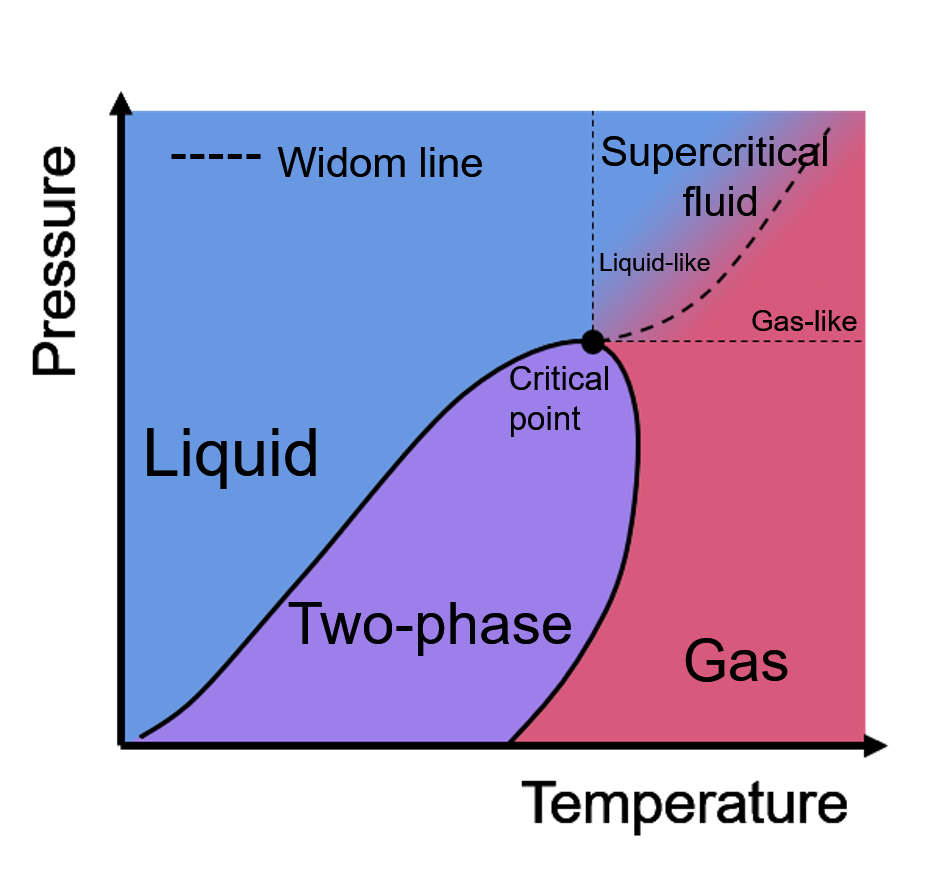
\includegraphics[width=0.5\linewidth]{TPdia.png}
            %\caption{fig1}
            %\end{minipage}%
        }%
        \caption{A P-T Diagram for a multicomponent system.}\label{TPdiagram}

    \end{figure}

\noindent\textbf{Models of transport properties:}

The dense fluid formulas in the Chung's method~\cite{chung1988generalized} are used to evaluate the dynamic viscosity $\mu$ and thermal conductivity $\lambda$. Chung's method is accurate for polar (e.g., \ce{H2O}), non-polar (e.g., \ce{CO2}, \ce{CH4}, \ce{O2}) and associating pure fluids and their mixtures at high pressures~\cite{chung1988generalized}. Meanwhile, its implementation is also straightforward. Chung's method has been widely used in a lot of studies of high pressure flows \cite{zhu2002model,trujillo2004high,yan2006high,matheis2018multi,tudisco2020vapor}, and in software such as CoolProp \cite{bell2014pure} and REFPROP \cite{lemmon2018nist}.
%Its dynamic viscosity and thermal conductivity have similar formulas:
%\begin{equation}
%    \lambda=\lambda_0 \lambda^*+\lambda_p \label{transp}
%\end{equation}
%where $\lambda$ represents dynamic viscosity or thermal conductivity. $\lambda_0$ is the gas property at low pressures (about 1 atm). $\lambda^*$ and $\lambda_p$ are high-pressure corrections. At high pressures, $\lambda_p$ is the major contributing term comparing to $\lambda_0 \lambda^*$. On the other hand, at low pressures, $\lambda^*$ is approaching unity, and the $\lambda_p$ term is negligible such that Eq.~(\ref{transp}) reduces to $\lambda_0$. Hence, the transition between subcritical regime and supercritical regime is smoothly described by the model. 
%For mass diffusivity, we used a simple Reynolds analogy, which yields a turbulent Schmidt number of 1. Hence, mass diffusivity is obtained from the dynamic viscosity and LES model.

For mas diffusivity $D_m$, the mixture-averaged mass diffusion model is used. Binary diffusion coefficient is evaluated by Fuller’s model~\cite{fuller1966new} with Takahashi’s correction~\cite{takahashi1975preparation}. Takahashi’s correction~\cite{takahashi1975preparation} is regarded as one of the most robust models at high pressures \cite{meng2005transport}, and is widely used in high pressure flow simulations \cite{xu2018validation,pohl2013real,nguyen2022real,ribert2017high}. % The mass diffusion coefficient of specie $i$, $D_i$, which is defined by \cite{kee1996chemkin}}

%\begin{equation}
%D_i=\frac{1-Y_i}{\sum^N_{j\neq i}X_j/D_{j,i}},\label{massdiff}
%\end{equation}
%\textcolor{\mycolor}{where $Y_i$ and $X_i$ are the mass and mole fractions of i-th species, respectively; }


\subsection{VLE-based CFD simulation framework}
\label{sec:model:cfd}

%Although the VLE theory has been proposed for a long while~\cite{hanks1971calculation} and 0D VLE calculation can be done by publicly available software such as the National Institute of Standards and Technology (NIST) Refprop~\cite{lemmon2018nist}, the development of VLE-based CFD solvers to capture high-pressure phase change just started during the past decade ~\citep{banuti2017phase,matheis2018multi,yao2019molecular,tudisco2020numerical,tudisco2020vapor,ray2019two,ma2018numerical}.~\citep{matheis2018multi,yao2019molecular,tudisco2020numerical,ray2019two}.
In this study, a high-pressure multiphase flow simulation framework is developed by coupling a pressure-based CFD solver with a VLE solver (the HPn flash): i.e., a VLE-based CFD simulation framework. %The compressible solver used in this research, is the sprayFoam solver in OpenFOAM, an open source C++ library based on the Finite Volume Method. 
The CFD solver is based on multicomponent governing equations, including the continuity equation, mixture momentum equations, mixture specific internal enthalpy equation, and transport equations of distinct components in the mixture, as follows:
\begin{align}
    % &\frac{\rho^*-\rho_n}{\Delta t}+\nabla\cdot(\rho_n U_n)=0\\
    % &\frac{\rho^*U^*-\rho_n U}{\Delta t}+\nabla\cdot(\rho_n U_n U^*)=-\nabla P_n+\nabla \cdot \tau\\
    % &\frac{\rho^*h^*-\rho_n h_n}{\Delta t}+\nabla\cdot(\rho_n U_n h)+\frac{\partial \rho K}{\partial t}+\nabla\cdot(\rho_n U_n K)-\frac{\partial P}{\partial t}=-\nabla \cdot q +\nabla \cdot (\tau\cdot U)\\
    % &U=HbyA_p-\frac{\nabla p}{A}\\
    % &\frac{\partial\phi P}{\partial t}+\nabla\cdot (\phi P (HbyA_p))-\nabla\cdot (\rho \frac{\nabla P}{A})=0\\
    % &\frac{\partial \rho}{\partial t}+\frac{\partial \rho u_i}{\partial x_i}=0\\
     & \frac{\partial \rho}{\partial t}+\frac{\partial \rho u_i}{\partial x_i}=0 \label{G:start}                                                                                                                                                                            \\
     & \frac{\partial \rho u_i}{\partial t}+\frac{\partial \rho u_i u_j}{\partial x_j}=-\frac{\partial p}{\partial x_i}+\frac{\partial \tau_{ij}}{\partial x_j} \label{Gm}                                                                                                   \\
    % &\frac{\partial \rho e}{\partial t}+\frac{\partial \rho e u_j}{\partial x_j}=-P\frac{\partial u_j}{\partial x_j}-\frac{\partial q}{\partial x_j}+\tau_{ij} \frac{\partial u_i}{\partial x_j}\\
     & \frac{\partial \rho h}{\partial t}+\frac{\partial \rho u_i h}{\partial x_i}+\frac{\partial \rho K}{\partial t}+\frac{\partial \rho u_i K}{\partial x_i}-\frac{\partial p}{\partial t}=-\frac{\partial q_i}{\partial x_i} +\frac{\partial \tau_{ij}u_j}{\partial x_i} \\
     & \frac{\partial \rho Y_m}{\partial t}+\frac{\partial \rho Y_m u_j}{\partial x_i}=\frac{\partial }{\partial x_j}\left(\rho \sum_m D_m \frac{\partial Y_m}{\partial x_j}\right) \label{G:end}
\end{align}
where $u_i$ is the velocity, $\rho$ and $h$ are the mixture density and internal enthalpy, respectively, $Y_m$ is the mass fraction of component $m$, $p$ is the pressure, $\tau_{ij}$ is the viscous stress tensor, $K$ is the kinetic energy, $q_i$ is the heat flux, and $D_m$ is the mass diffusivity of component $m$.
In this study, $q_i=-\alpha \nabla h$ where $\alpha$ is the thermal diffusivity. In the relevant systems of this study (mixture: \ce{CH4}/\ce{CO2}/\ce{H2O}, \ce{O2}/\ce{CO2}/\ce{H2O}; $p$: $10^7$ Pa; $T$: 300-700 K), the Lewis numbers ($Le_m=\alpha/D_m$) are obtained using the models mentioned in Sec.~\ref{thermo models}, and their values are in the range of $O(10^3)$ $\sim$ $O(10^5)$. Hence, the contribution of mass diffusion to energy flux is weak, and it is neglected in this study.

The OpenFOAM solver uses the PIMPLE algorithm ~\cite{holzmann2016mathematics}, which is a combination of the SIMPLE (semi-implicit method for pressure-linked equations) \cite{patankar1983calculation} and PISO (pressure-implicit split-operator) algorithms \cite{issa1986solution} based on the primitive variables (e.g., pressure $p$). The implementation of the PIMPLE algorithm in OpenFOAM has been validated by a lot of researchers around the world for different thermofluid applications~\cite{robertson2015validation, higuera2014three,gaikwad2019openfoam,gamet2020validation,de2017implementation,ashton2019verification}. Additional validation and verification of the CFD solver are provided in Appendix~\ref{App:vali:CFD}, including two shock tube cases and a jet-in-cross flow case. In the original solver, the SIMPLE algorithm is used to predict $\rho$, $u_i$, $h$, and $Y_m$ from Eqs.~(\ref{G:start}-\ref{G:end}), in every time step (i.e., the outer loop in Fig.~\ref{FC_CFD}). Then, thermodynamic properties, including $T$ (mixture temperature) and $\phi$, are evaluated from the $p$ in the last step and the updated $h$ and $Y_m$ using thermodynamic model. The ideal gas model and Peng-Robinson Equation of State, PR-EOS, are provided in the standard OpenFOAM version. $\phi$ is used to update $p$ and calculate $\rho$. Then, transport properties are updated accordingly. %This is why the HPn flash solver is used to couple with the CFD solver based on the primitive variables. %Please note that this VLE-based CFD simulation framework does not assume isobaric and isenthalpic.
Here, $\phi$ is defined as
\begin{align}
     & \phi = \frac{\rho} {p}, \label{EOS}
\end{align}
in which the specific form of $\phi$ depends on the choice of thermodynamics model. %  whether VLE is used and which EOS is used (e.g., ideal gas EOS and PR-EOS). This marks the end of the predictor step.
%The CFD solver is developed base on SprayFoam, a OpenFOAM solver designed for compressible, turbulent flow with a spray particle cloud. In this study, we took advantage of its 
Then $p$ is updated iteratively by solving its Poisson equation. %several times (3 times used in this study).
Velocity $u_i$ and thermodynamic properties ($\rho$, $T$, $\phi$, etc.) are also updated after solving the pressure equation at each iteration step.
%\comment{until it converges.} 
This inner iteration is from the PISO algorithm, and hence it is called PISO loop, as shown in Fig.~\ref{FC_CFD}. %Details about the pressure Poisson equation and its numerical treatment are shown in Appendix~\ref{App:gp}. 
 %This mark the end of the corrector step. 
When PISO loop finshed, $\rho$ is updated using Eq.~(\ref{EOS}). 
With the updated properties, Eqs.~(\ref{Gm}-\ref{G:end}) are solved iteratively to update $u_i$, $h$, and $Y_m$, respectively, using the semi-implicit method (i.e., the predictor step) until it converges. This iteration is from the SIMPLE algorithm, and hence is called SIMPLE loop, as shown in Fig.~\ref{FC_CFD}. When SIMPLE loop finished, the next time step starts.

%This CFD solver is capable of solving subsonic and transonic flows with and without reactions. It uses Pressure-Implicit with Splitting of Operators (PISO) method \citep{karrholm2006rhie} for solving the governing equations, which includes a predictor step and multiple corrector steps. %Using PISO, velocity and pressure can be directly solved by the following equations: 

\begin{figure}[htbp]
    \centering
    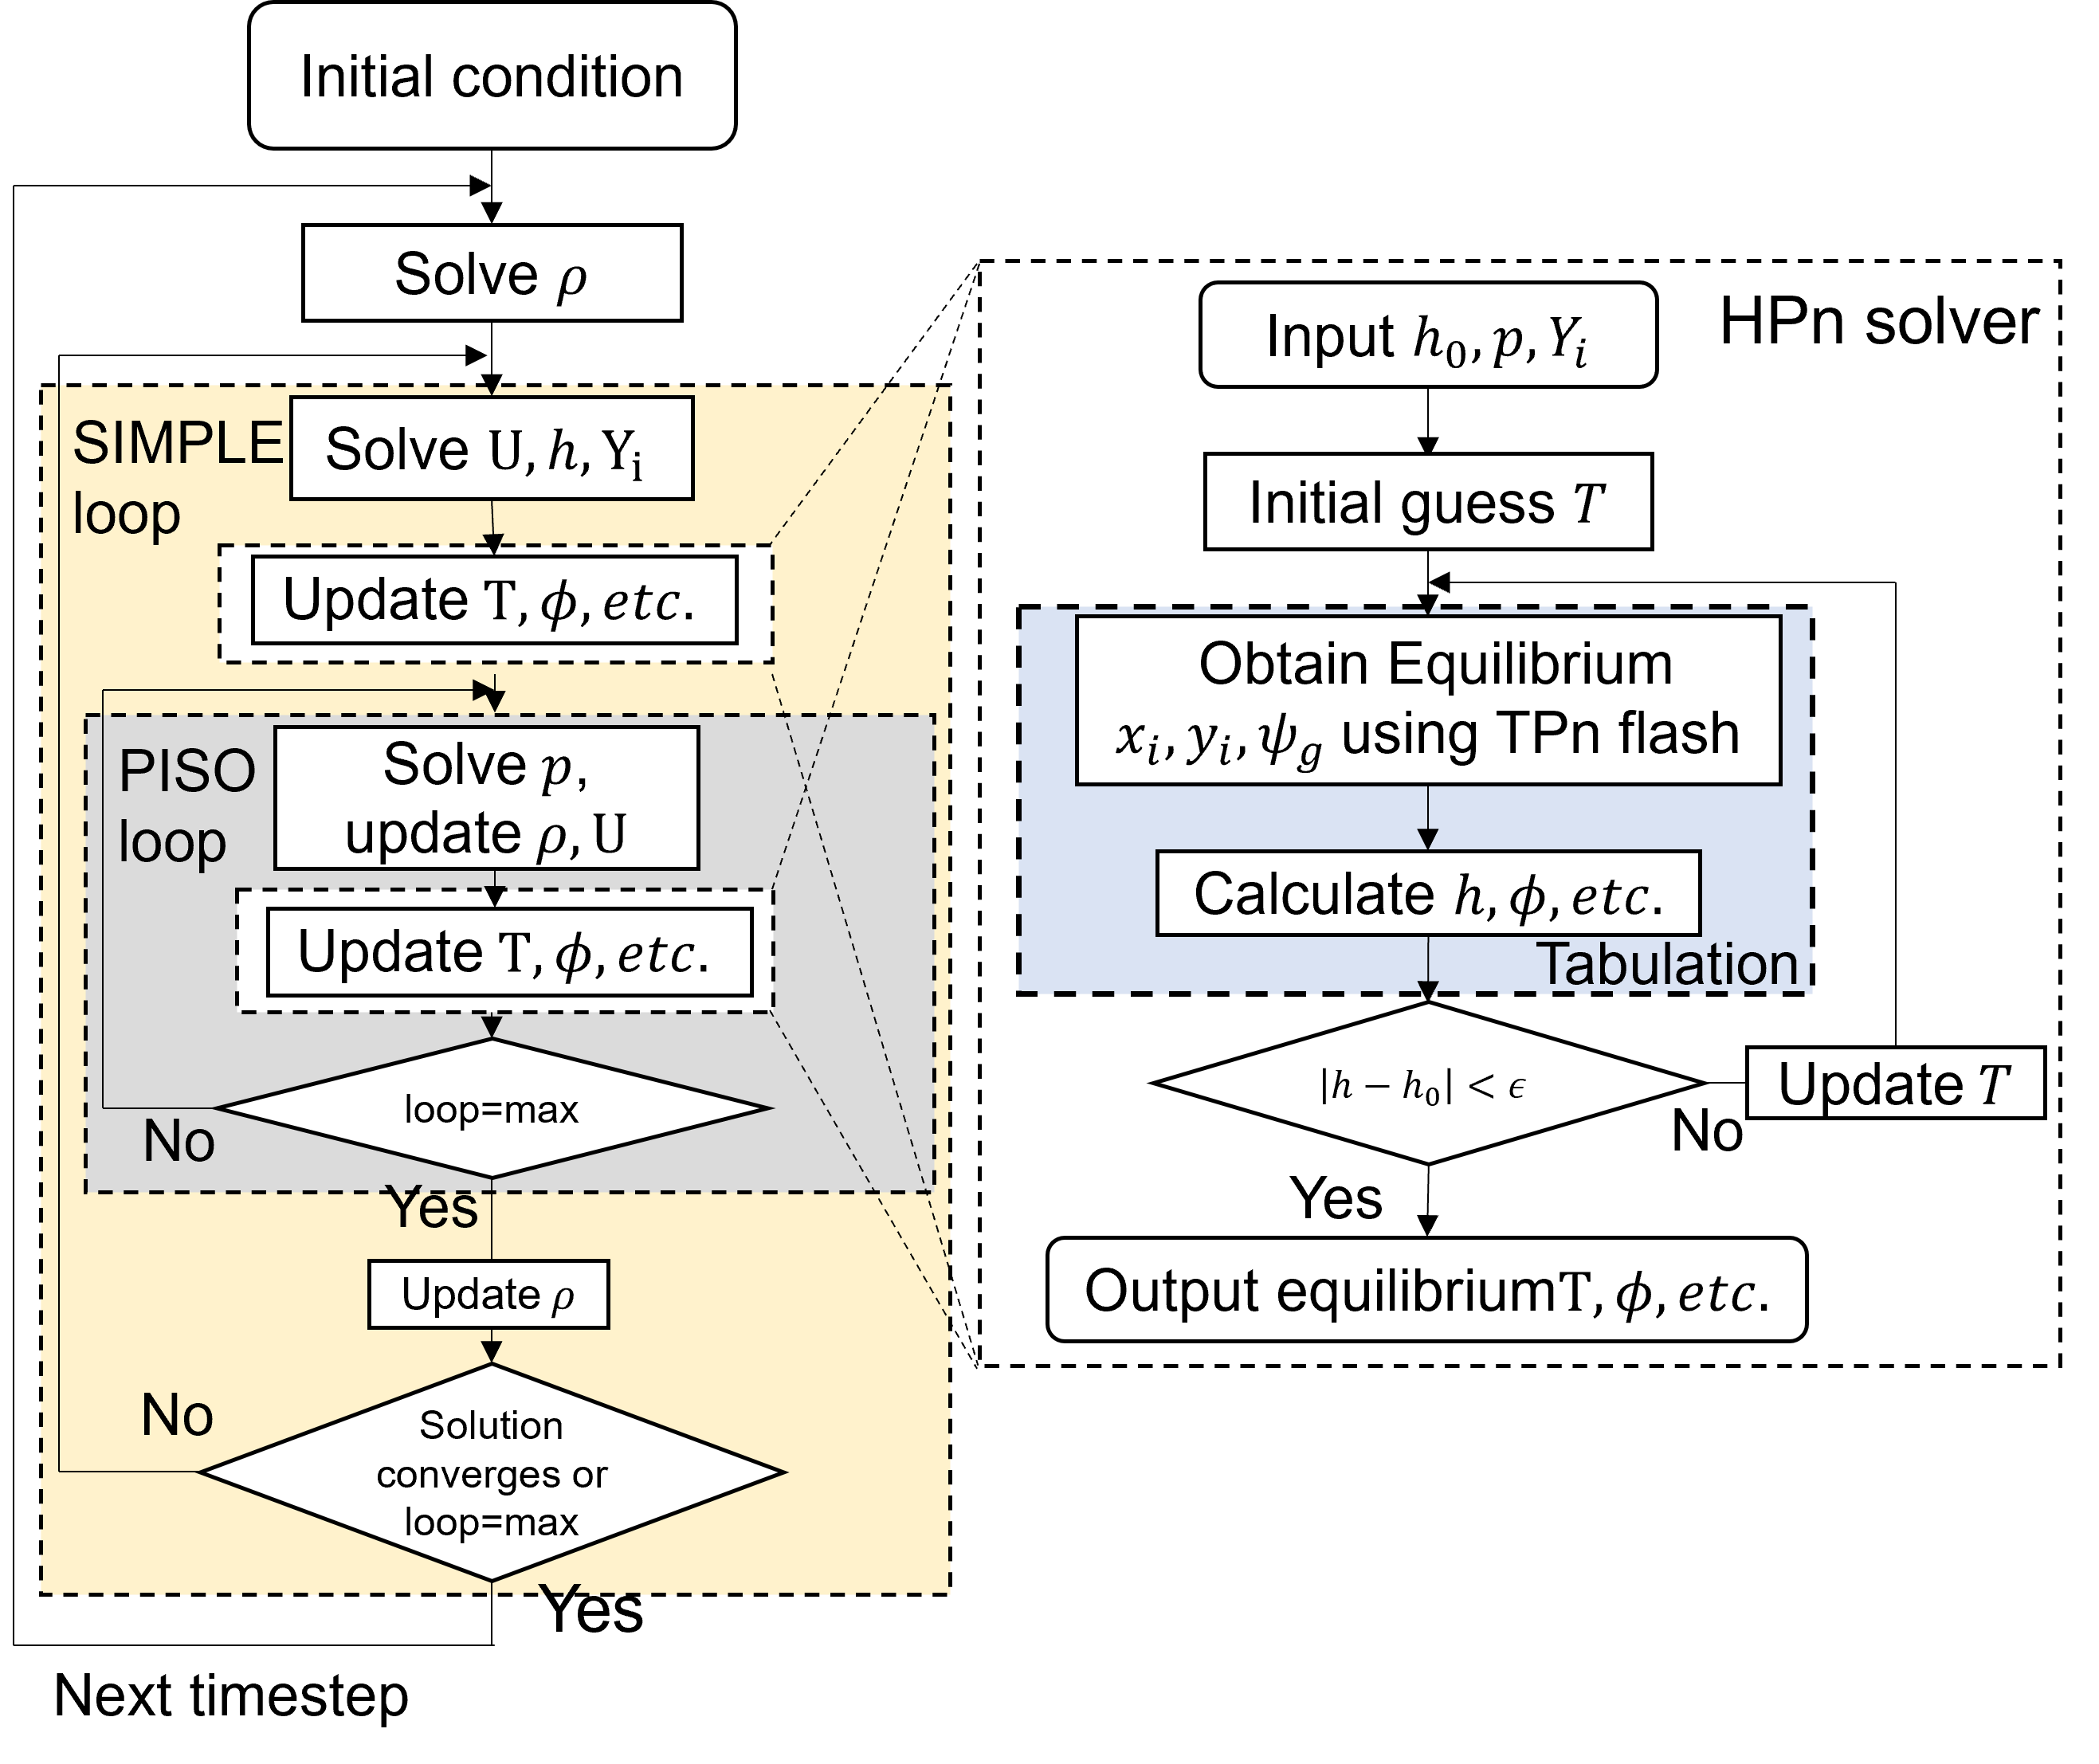
\includegraphics[width=0.95\linewidth]{flowchart.png}
    \centering
    \caption{Flow chart of the VLE-based CFD solver.}
    \label{FC_CFD}
\end{figure}

The new contributions from this study to the OpenFOAM solver and PIMPLE algorithm are summarized here. 
%The thermal properties are updated at each step, which are usually determined by a equation of state. In this investigate, VLE is also taken into account. 
%At each step, the CFD solver updates fluid properties, including mixture density $\rho$, mixture enthalpy $h$, and mass fraction $Y_m$, which are enough to determine the thermal equilibrium state. 
%Since VLE theory is used to update thermodynamics properties ($T$, $\phi$, etc.), the equilibrium state is assumed to be achieved ``immediately" at every grid point.
%In the simulation, the equilibrium state
%is assumed to be achieved immediately at every grid point, and this equilibrium state can be obtained from the VLE solver. Hence, by sothermodynamicted for the next time step, which is shown in Fig.~\ref{FC_CFD}. 
This study replaces the original thermodynamic model with the VLE + PR-EOS model implemented in this study, as shown in Fig.~\ref{FC_CFD}.
Due to the high computational cost of VLE calculation, %Yi et al.~\citep{yi2019numerical} used a simple tabulation method to accelerate the simulation and make the solver computationally more affordable. In this work, 
a novel VLE-based tabulation method is developed to accelerate simulations and make the CFD solver computationally more affordable, as shown in the right box of Fig.~\ref{FC_CFD}. For each simulation, a table is generated to record the solution of TPn flash, density, enthalpy, $c_p$, and transport properties at different temperatures (280-1200 K), pressures (280-700 bar), and \ce{CO2} mole fractions (0.0001-0.9999). Each solution includes, every species' mole fraction in liquid and gas phases, and transport properties. In simulations, a linear approximation method based on eight neighboring records is used for data retrieval. More details about this VLE-based tabulation method is provided in Appendix~\ref{App:tab}. For a large number of components, this tabulation method will demand infeasible memory, and we are developing a new on-the-fly tabulation of VLE solutions using the \textit{in situ} adaptive tabulation (ISAT) approach~\cite{zhang2021multi}, similar to the idea of correlated dynamic evaluation of real fluid properties for supercritical mixing~\cite{yang2017comparison} and combustion~\cite{milan2019time}.


\section{Results and Discussion}
\label{sec:result}

%\subsection{Mixture critical point and phase separation at conditions relevant to \ce{sCO2} compressors and turbines}
%\label{sec:result:compressor}

%One of the advantages of traditional closed \ce{sCO2} cycle is that the \ce{CO2} is a single-phase supercritical working fluid, which does not create the associated thermal fatigue or erosion like the subcritical two-phase working fluids. On the other hand, since the compressibility of the supercritical liquid-like \ce{CO2} is very low, it needs less compression work in the compressor, which can improve the thermal efficiency~\citep{ahn2015review,invernizzi2017prospects}. However, for the semi-closed \ce{sCO2} gas turbine systems with oxy-combustion, the mixtures of \ce{CO2}/\ce{H2O} (instead of pure \ce{CO2}) out from the recuperator need to pass through the compressor (see Fig.~\ref{fig1} in \ref{app:sCO2cycle}). The thermodynamic states for such mixtures are different from pure \ce{CO2} and hence the above advantage of \ce{sCO2} systems also need to be re-evaluated.
To investigate the effects of phase separation in \ce{sCO2} systems, 0D thermodynamics analyses are first performed to discover the conditions under which phase separation could occur (in Sec.~\ref{sec:results:ThermAnalysis}). In Sec.~\ref{sec:results:ShockTube}, 1D shock tube simulations are conducted to understand the effect of the phase change model compared with two models without phase change, and understand the interaction between phase separation and compression/expansion waves. In Sec.~\ref{sec:results:JICF}, we performed 3D jet-in-crossflow LES to discuss the influence of mixing on phase separation. 

\subsection{0D thermodynamics analyses of the \ce{sCO2} systems}
\label{sec:results:ThermAnalysis}

In a real flow, many factors (e.g., boundary condition, turbulence, temperature perturbation) affect the fluid flow, making it difficult to analyze thermodynamic properties. Hence, in this section, 0D thermodynamics analyses are performed to give insights into the thermodynamic properties without the influence of other factors. First, the mixture critical points are calculated to show the influence of impurities in Sec.~\ref{sec:results:combustor:H2O}. Then, the influence of the critical point on thermodynamic properties is discussed in Sec.~\ref{sec:results:combustor:phase}. Since isenthalpic mixing is similar to what often happens in the real \ce{sCO2} systems, in the end, the two-phase region in the isenthalpic mixing process is discussed (in Sec.~\ref{sec:results:combustor:HPn}). 

%\subsubsection{Influence of \ce{H2O} addition on the mixture phase diagrams near the fuel injector}
\subsubsection{Influence of impurities on premixed \ce{sCO2} systems: elevated critical point and retrograde condensation}
\label{sec:results:combustor:H2O}

    %\section{Analysis of thermodynamics of \ce{sCO2} compressors: phase separation and its  influence}  \label{thermo analysis}
    %In \ce{sCO2} compressors, the supercritical fluid, such as \ce{sCO2}, holds high energy density $\rho e$ near its critical point due to the large variation of density $\rho$, which results in a large change in specific heat capacity $c_p$ for a small temperature change. Therefore, it is better to keep the fluid temperature close to the critical point to take this special advantage of high energy density to compact the turbomachinery.
    %Both subcritical liquid fluid and supercritical liquid-like fluid have low compressibility to reduce the compression work necessary for a given pressure ratio \citep{ahn2015review,invernizzi2017prospects}, which is a motivation to keep the working fluid close to its critical point so that the compressor can work under these conditions. Accordingly, an accurate determination of the mixture critical point becomes very important. 
    %In this section, the evolution of mixture critical point and the compressibility in the compressor is evaluated.

As discussed before, the injection of fuel (e.g., \ce{CH4}) and oxidizer (e.g., pure \ce{O2} or air) and the combustion products (e.g., \ce{H2O}) can introduce many impurities to the \ce{sCO2} systems. Accordingly, this section will investigate the mixture phase diagrams of \ce{sCO2} systems with different combinations of impurities, including both two-component and three-component systems (also see Appendix~\ref{app:trad} and Sec.~\ref{sec:results:combustor:phase} for four-component systems).

    \begin{figure}[htb]
        \centering
        \subfigure{
            %\begin{minipage}[t]{0.5\linewidth}
            \centering
            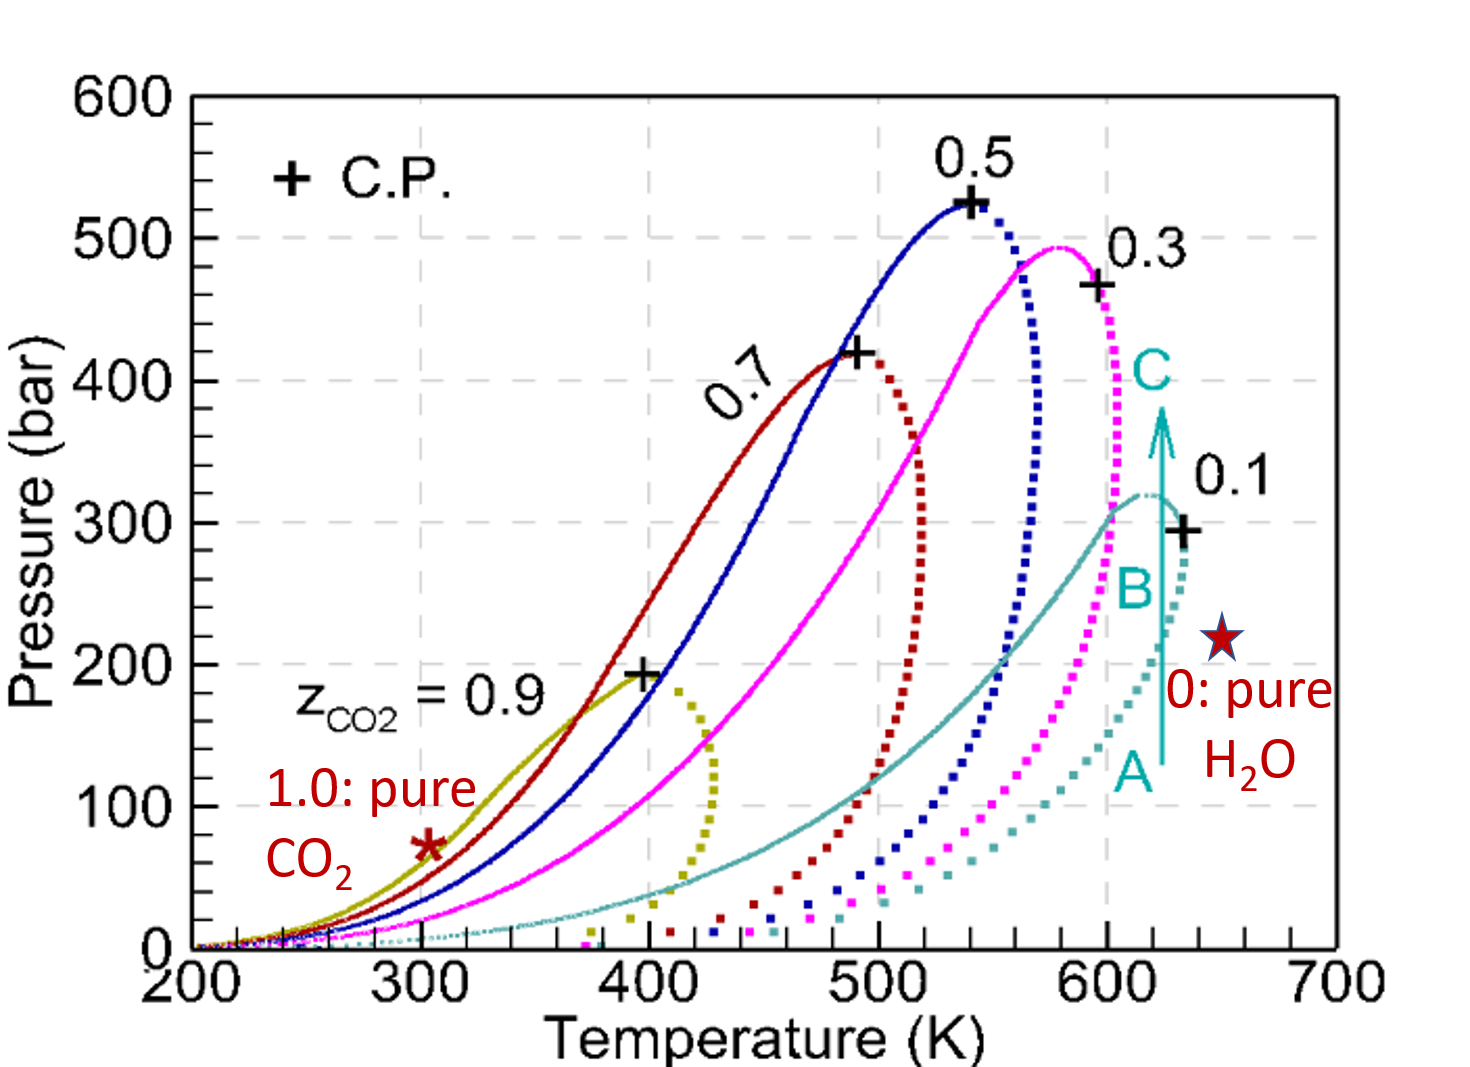
\includegraphics[width=0.5\linewidth]{phase_diagram_PT_CO2_H2O.png}
            %\caption{fig1}
            %\end{minipage}%
        }%
        \caption{Pressure-temperature phase boundaries and mixture critical points of \ce{CO2}/\ce{H2O} mixtures with different mole fraction values of \ce{CO2} (i.e., $z_{CO_2}$). Note the retrograde condensation behavior from A to B to C.}\label{v3}

    \end{figure}

As an example of two-component \ce{sCO2} systems, the pressure-temperature phase diagram of \ce{CO2}/\ce{H2O} mixtures is generated by the TPn flash solvers~\cite{michelsen1982isothermal} (see details in the Supplementary Material of this article) and shown in Fig.~\ref{v3}. %The compressibility of this mixture with a feed of \ce{CO2}/\ce{H2O}=0.3/0.7 is shown in Fig.~\ref{v3}(b).
The mixture critical pressures can be significantly higher than the critical pressure of each individual component (i.e., pure \ce{CO2} and pure \ce{H2O}).
As a result, at conditions close to the critical point of pure \ce{CO2} (304.13 K, 73.78 bar), the \ce{CO2}/\ce{H2O} mixtures (with $\ge10\%$ \ce{H2O}) are in subcritical liquid phase. Therefore, a so-called ``supercritical \ce{CO2}'' system might be in a subcritical state due to the rise of mixture critical points caused by some impurities. In order to get a supercritical state for the \ce{CO2}/\ce{H2O} mixtures, the pressure and temperature need to be elevated about 100-200 K and 100-500 bar, respectively. %If the temperature and pressure are still close to those in the traditional closed \ce{sCO2} systems, the mixtures in the compressors of \ce{sCO2} gas turbine systems will be in liquid phase, which could cause erosion.
In addition, retrograde condensation behavior could occur in such systems. % Retrograde condensation behavior has been explained in Sec.~\ref{app:trad}.%: 
Specifically, when the subcritical gas (at Point A) is compressed into the subcritical two-phase zone, phase separation could occur, and the gas partially condenses into liquid (at Point B), but further compression makes the mixture go outside of the two-phase zone such that the liquid component (at point B) evaporates again (i.e., the so-called ``retrograde condensation") to Point C. Similar but the reverse process occurs during the expansion from Point C to Point A.
%\ce{CO2}/\ce{CH4} mixtures exist near the fuel injector in a \ce{sCO2} oxy-combustor. The mixtures with $z_{\ce{CO2}}$ from 0 to 1 are the jet-in-crossflow mixtures from the fuel injector to the end of the penetration length. Since \ce{sCO2} oxy-combustors always contain some water (e.g., the cooler cannot remove all water generated by the last cycle's combustion), it influences the thermodynamic state of the mixture. As a result, even the typical working conditions (100-300 or 400 bar, 300-1000 K) may overlap with the two-phase zone. Accordingly, this section investigates the influence of different levels of \ce{H2O} addition on the \ce{CO2}/\ce{CH4} mixture phase diagrams. %In the literature, the phase diagram as well as the tangent plane distance (TPD) method are commonly used to justify the phase state. %(??)Both the phase state and TPD are validated for single component, but are invalidated for multicomponent mixture because their values are affected by the feed, which is determined by the mixing process. 
As another example of two-component \ce{sCO2} systems, Figure~\ref{v5}(a) shows the thermodynamic states of \ce{CO2}/\ce{CH4} mixtures. Similar to the \ce{CO2}/\ce{H2O} mixtures in Fig.~\ref{v3}, the mixture critical pressures of \ce{CO2}/\ce{CH4} can also be higher than those of both pure \ce{CH4} and pure \ce{CO2}.

%With the help of \ce{CO2}, significant higher critical pressures can be obtained compared to typical gas turbine engines in Fig.~\ref{v4}(a). 

%However, the typical working conditions are still far away from the two-phase zones of all possible \ce{CO2}/\ce{CH4} mixture compositions. Thus the mixtures are always in supercritical gas-like states.

\begin{figure}[htb]
    \centering

    \subfigure{
        \begin{minipage}[t]{1\linewidth}
            \centering
            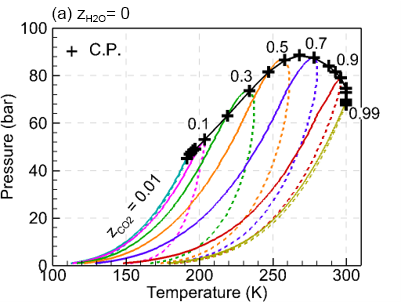
\includegraphics[width=0.45\linewidth]{phase_diagram_PT_CO2_CH4.png}
            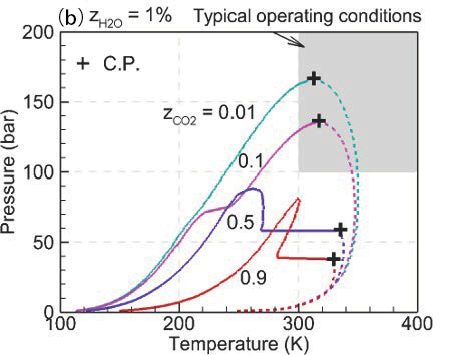
\includegraphics[width=0.45\linewidth]{phase_diagram_PT_CO2_CH4_1_H2O.png}
            %\caption{fig1}
        \end{minipage}%
    }%

    \subfigure{
        \begin{minipage}[t]{1\linewidth}
            \centering
            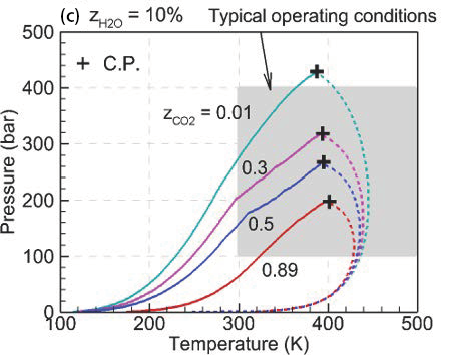
\includegraphics[width=0.45\linewidth]{phase_diagram_PT_CO2_CH4_10_H2O.png}
            %\caption{fig2}
        \end{minipage}%
    }%
    \caption{Effects of \ce{H2O} addition on the pressure-temperature phase boundaries and critical points of \ce{CO2}/\ce{CH4}/\ce{H2O} mixtures: (a) no \ce{H2O} addition; (b) 1\% \ce{H2O} addition; (c) 10\% \ce{H2O} addition.}
    \label{v5}
\end{figure}

As an example of three-component \ce{sCO2} systems, Figure~\ref{v5} shows the influence of different levels of \ce{H2O} addition on the \ce{CO2}/\ce{CH4}/\ce{H2O} mixture phase diagrams.
As shown in Fig.~\ref{v5}(b), even only 1\% of \ce{H2O} addition can increase the mixture critical point significantly. When the amount of \ce{CO2} is sufficiently small (e.g., $z_{CO_2}\leq0.1$), the mixture critical pressure can be larger than 100 bar. %make the two-phase zone enter the typical operating conditions if the amount of \ce{CO2} is sufficiently small (e.g., $z_{CO_2}\leq0.1$). But when there is a large amount of \ce{CO2} in the mixture (e.g., $z_{CO_2}\geq0.5$), the operating conditions could be purely supercritical and gas-like. Therefore, phase separation could occur near the fuel injector, but its region might be small.
As shown in Fig.~\ref{v5}(c), when $z_{H_2O}$ rises to 10\%, the mixture critical point increase even further. The mixture critical pressure can range from 200 to 400 bar.
The typical working condition range of \ce{sCO2} oxy-combustors (100-400 bar and $\ge300$ K) is indicated in Fig.~\ref{v5}. With \ce{H2O} addition, that working condition range overlaps with the subcritical two-phase zone, indicating that phase separation could occur.
%the operating conditions always intersect with the two-phase zone regardless of the amount of \ce{CO2} in the mixture. As a result, phase separation occurs through a large portion of the fuel jet until the temperature is sufficiently high.
Another typical three-component \ce{sCO2} systems are the \ce{CO2}/\ce{CH4}/\ce{O2} systems, which are investigated in Appendix~\ref{app:trad} and show similar retrograde condensation behavior as the \ce{CO2}/\ce{H2O} systems in Fig.~\ref{v3}.


\subsubsection{Influence of mixture critical point and phase change on the thermodynamic properties of the \ce{sCO2} systems}
\label{sec:results:combustor:phase}
The mixture critical point and phase change affect all mixture thermodynamic properties, because all of them are functions of reduced pressure ($p_r=p/p_c$) and reduced temperature ($T_r=T/T_c$), especially when the thermodynamic state is close to the critical point and/or deviates from ideal gas (typically high $p$ low $T$ conditions). %, as shown in Appendix~\ref{app:compressibility}). %Among these properties, the density, specific heats, thermal conductivity, mass diffusivity, speed of sound and internal energy are largely affected.

    %\comment{The previous section has shown that the typical working conditions of \ce{sCO2} oxy-combustors can encounter the two-phase zone, and hence phase separation can occur. But the influence of phase separation on the fluid properties is still unclear, which is investigated in this section.
    %This section investigates the influence of phase separation on the fluid properties.}

    %To avoid repeating the same information,

    %In oxy-combustors, the locations where \ce{CH4} and \ce{O2} have mixed but not yet reached an ignition or a flame are considered here. At such locations, the \ce{CO2} concentration is very high, so its concentration is assumed to be 90\%. Due to the cooler, the \ce{H2O} concentration is typically low in \ce{sCO2} combustors, so its concentration is assumed to be 1\%. Without loss of generality, the concentration of \ce{CH4} and \ce{O2} are both assumed to be 4.5\%.

     Figure~\ref{fig:PTdiagram_rho} shows the density of the mixture with and without phase separation. Comparing to the $z_{\ce{CO2}}=0.9$ curve in Fig.~\ref{v5}(b), it is seen that with the addition of \ce{O2}, the mixture critical pressure further rises from below 50 bar to approximately 350 bar. As a result, a significant part of the typical working conditions overlaps with the subcritical two-phase zone to trigger phase separation. By comparing Fig.~\ref{fig:PTdiagram_rho}(a) and (b), it is seen that at the relevant conditions of this work (i.e., 100-300 bar), phase separation only has a small influence on the density of this specific mixture. This indicates that the assumption of ``supercritical dense gas-like fluid" in Fig.~\ref{fig:PTdiagram_rho}(b) could result in a similar mixture density as the real subcritical two-phase mixture in Fig.~\ref{fig:PTdiagram_rho}(a) at the same thermodynamic condition.

    \begin{figure}[htb]
        \centering

        \subfigure{
            \begin{minipage}[t]{1\linewidth}
                \centering
                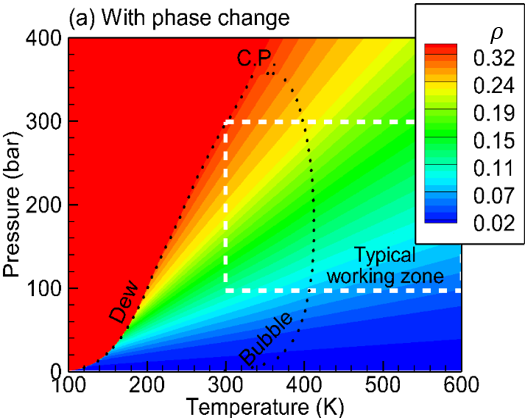
\includegraphics[width=0.45\linewidth]{rho_PT_VLE.png}
                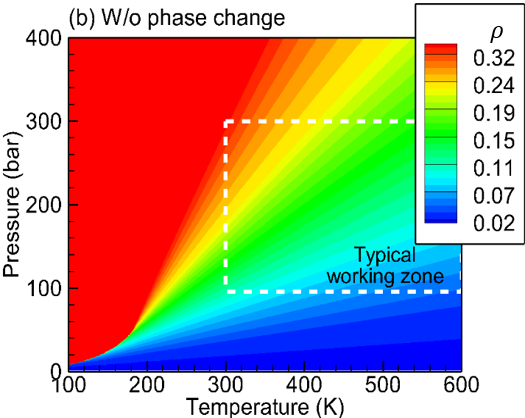
\includegraphics[width=0.45\linewidth]{rho_PT_noVLE.png}
                %\caption{fig1}
            \end{minipage}%
        }%

        \caption{Density ($\rho$) of \ce{CO2}/\ce{H2O}/\ce{CH4}/\ce{O2} mixture with an overall mole fraction of 0.9/0.01/0.045/0.045 in the pressure-temperature phase diagram: (a) with phase change (i.e., with VLE); (b) without phase change (i.e., without VLE).}
        \label{fig:PTdiagram_rho}
    \end{figure}

    In contrast, Figure~\ref{fig:PTdiagram_cp} shows that phase separation has a considerable influence on the isobaric heat capacity of the mixture. This could significantly affect the heating/evaporating timescale of the mixture and consequently, affect the ``effective" ignition delay in the cold ignition process.

    \begin{figure}[htb]
        \centering

        \subfigure{
            \begin{minipage}[t]{1\linewidth}
                \centering
                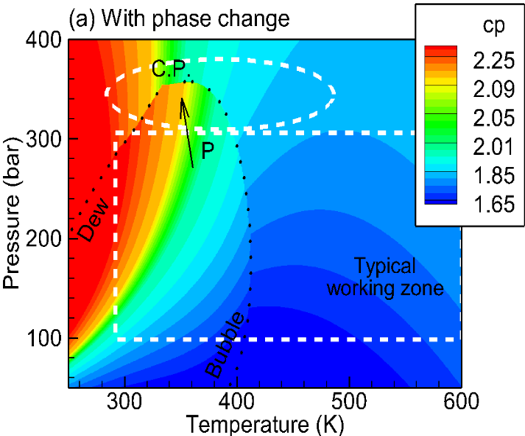
\includegraphics[width=0.45\linewidth]{cp_PT_VLE.png}
                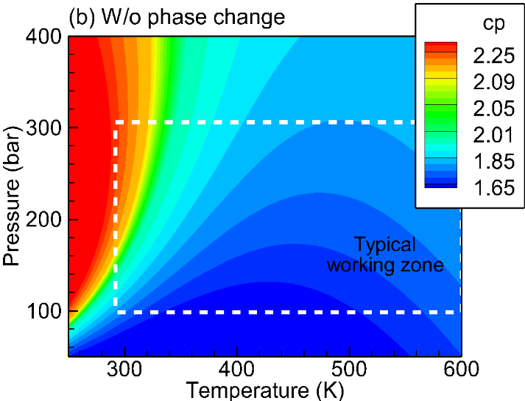
\includegraphics[width=0.48\linewidth]{cp_PT_noVLE.png}
                %\caption{fig1}
            \end{minipage}%
        }%

        \caption{Isobaric heat capacity ($c_p$) of \ce{CO2}/\ce{H2O}/\ce{CH4}/\ce{O2} mixture with an overall mole fraction of 0.9/0.01/0.045/0.045 in the pressure-temperature phase diagram: (a) with phase change (i.e., with VLE); (b) without phase change (i.e., without VLE).}
        \label{fig:PTdiagram_cp}
    \end{figure}


%\subsubsection{Subcritical and supercritical mixing and phase separation in \ce{sCO2} oxy-combustors}
%\label{sec:results:combustor:HPn}
\subsubsection{Isobaric and isenthalpic (HPn) mixing in the \ce{sCO2} systems: \ce{H2O}-induced low-T phase separation} \label{sec:results:combustor:HPn}
The previous analyses %for \ce{sCO2} oxy-combustors
are based on the pressure-temperature phase diagrams generated by the isothermal and isobaric (TPn) flash solver~\cite{michelsen1982isothermal}.
%In real \ce{sCO2} oxy-combustors,
However, many real mixing processes follow the isobaric and isenthalpic (HPn) path \cite{serrano2018development}. Thus the real phase states should be determined based on the isenthalpic mixing process generated by the HPn flash solver~\cite{michelsen1987multiphase}. Details of both TPn and HPn flash solvers are provided in Michelsen's works~\cite{michelsen1982isothermal,michelsen1987multiphase} and the Supplementary Material of this article.
%, which was discussed in Sec.~\ref{thermo models}.
%All analyses above are based on temperature and pressure using TPn flash solver, but for isentropic mixing process, HPn flash is more suitable to describe phase split in mixing processes. 
%Here, we are going to analyze the isentropic mixing process in combustor using HPn flash result.

Based on Fig.~\ref{v7}, for the mixing between 300 K \ce{CH4} and 900 K \ce{CO2} without \ce{H2O}, it is in a supercritical gas-like state during the whole mixing process, which agrees with the observation from the pressure-temperature phase diagram in Fig.~\ref{v5}(a). Note that although not shown here, the same conclusion is observed when the ambient temperature of \ce{CO2} is below 700 K.
%This is confirmed by tangent plane distance (TPD) phase stability test \citep{michelsen1982isothermal}, which is a number of numerical methods for stability analysis based on Gibbs’ tangent plane criterion, in Fig.~\ref{v7} as expected.
\begin{figure}[htb]
    \begin{center}
        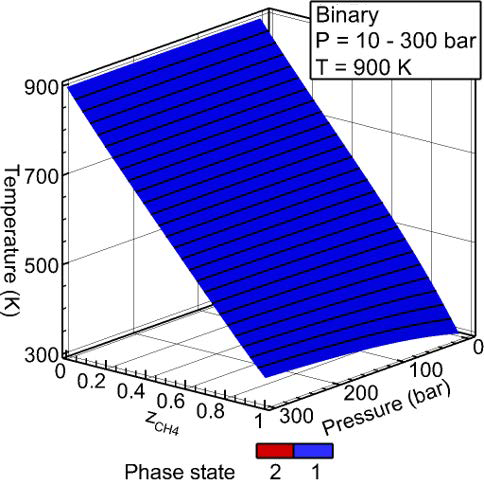
\includegraphics[width=0.4\linewidth]{mixing_temperature_CO2_CH4.png}
    \end{center}
    \caption{Equilibrium mixing temperature $T_{eq}$ for the mixing between 900 K \ce{CO2} and 300 K \ce{CH4}: the pressure is in the range of 10 – 300 bar, and the overall mole fraction of \ce{CH4} is in the range of 0.01 – 0.99. Red: two-phase zone; blue: single-phase zone.}
    \label{v7}
\end{figure}

As shown in Fig.~\ref{v8}, with the help of \ce{H2O}, the subcritical two-phase zone can start to play an important role. %For the mixture of \ce{CO2}/\ce{CH4}/\ce{H2O}%, superimposing the true adiabatic mixing temperature (TAMT) is on the mixture critical locus line, the two-phase region can be easily determined. 
For the mixing between \ce{CH4} (300 K) and \ce{CO2}/\ce{H2O} mixture, if the ambient temperature (i.e., the temperature of \ce{CO2}/\ce{H2O} mixture) is lower than 700 K (i.e., Fig.~\ref{v8} (a-b)), the mixture can pass through the subcritical two-phase zone. The area of the two-phase zone increases as the pressure increases from 100 bar to 400 bar. When the ambient temperature reaches 900 K in Fig.~\ref{v8}(c), the mixing process does not pass the subcritical two-phase zone, so there is no more phase separation. Hence, for \ce{sCO2} systems with low temperatures (e.g., 700 K or lower), \ce{H2O} can cause phase separation. But for high-temperature \ce{sCO2} systems (e.g., 900 K or higher), phase separation cannot happen.  %\comment{But this ambient temperature is possible only near the fuel injectors and too low for the downstream locations of real \ce{sCO2} oxy-combustors. Based on the literature \citep{delimont2017direct}, the auto-ignition occurred at high concentrations of \ce{CO2} at least 900 K (i.e., Fig.~\ref{v8}(c)). For the lowest auto-ignition temperature (i.e., 900 K) and highest pressure (i.e., 400 bar), the mixing process still does not pass the two-phase zone, so there is no phase separation.}
\begin{figure}[htb]
    \centering
    \subfigure{
        \begin{minipage}[t]{1\linewidth}
            \centering
            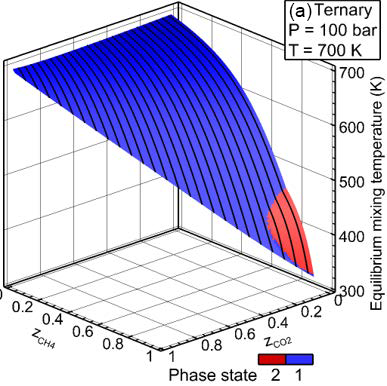
\includegraphics[width=0.32\linewidth]{mixing_temperature_CO2_CH4_H2O_100bar_700k.png}
            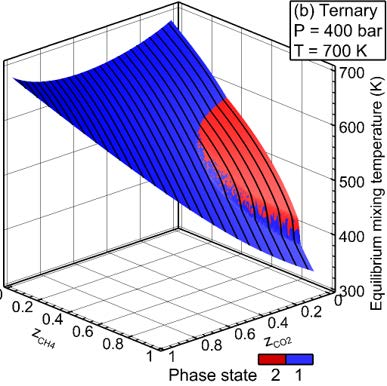
\includegraphics[width=0.32\linewidth]{mixing_temperature_CO2_CH4_H2O_400bar_700k.png}
            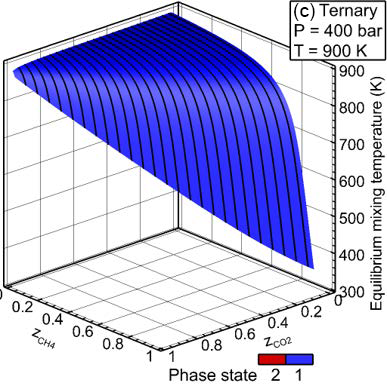
\includegraphics[width=0.32\linewidth]{mixing_temperature_CO2_CH4_H2O_400bar_900k.png}
            %\caption{fig1}
        \end{minipage}%
    }%

    \caption{Equilibrium mixing temperature $T_{eq}$ for the mixing between \ce{CH4} at 300 K and \ce{CO2}/\ce{H2O} mixture at the ambient pressure and temperature of (a) 100 bar and 700 K; (b) 400 bar and 700 K; and (c) 400 bar and 900 K. Red: two-phase zone; blue: single-phase zone.}
    \label{v8}
\end{figure}


%\subsection{VLE-based CFD solver}
%\textbf{1D advection tube of \ce{CO2}/\ce{H2O} mixture:}
%To test the robustness of the VLE-based CFD solver, an advection tube simulation is conducted, and its detailed configuration is shown in Fig.~\ref{adv_sc}. Figure~\ref{adv}(a-b) shows sharp temperature and density change at the two phase interfaces. In addition, the phase split is also captured by the CFD solver which is shown in the vapor fraction plot Fig.~(\ref{adv_sc})c. More \ce{H2O} in the mixture makes it harder to evaporate, and vapor fraction decreases. Hence, the jump of vapor fraction indicate the phase interface between mixtures with different concentrations.
%\begin{figure}[htbp]
%\centering
%\subfigure{
%\begin{minipage}[t]{1\linewidth}
%\centering
%\includegraphics[width=0.9\linewidth]{adv/adv_sc.png}
%\end{minipage}%
%}
%\caption{Configuration of the advection tube.}
%\label{adv_sc} 
%\end{figure}

%\begin{figure}[htbp]
%\centering
%\subfigure{
%\begin{minipage}[t]{1\linewidth}
%\centering
%\includegraphics[width=0.45\linewidth]{adv/av_t.png}
%\includegraphics[width=0.45\linewidth]{adv/av_rho.png}
%\end{minipage}%
%}\\
%\subfigure{
%\begin{minipage}[t]{1\linewidth}
%\centering
%\includegraphics[width=0.45\linewidth]{adv/av_vf.png}
%\end{minipage}%
%}%
%\caption{Simulation results of advection tube with \ce{CO2}/\ce{H2O} mixture, at $t=5\times10^{-6}s$: (a) temperature; (b) density; and (c) vapor fraction.}
%\label{adv} 
%\end{figure}


%\subsubsection{Phase change effect on thermodynamic properties} 
%The difference between transcritical model and ideal gas model comes from real gas effect and phase change. Here, phase change effect on thermodynamic and transport properties is investigated. The plots of $c_p$, Fig.~\ref{phasechange:cp}, are generated by TPn flash to compare the effect of phase change. In Fig.~\ref{phasechange:cp},  in typical working zone but with low fluid temperature, the predicted $c_p$ in two-phase zone is different with that without phase change

%\begin{figure}[htbp]
%\centering
%\subfigure{
%\begin{minipage}[t]{1\linewidth}
%\centering
%\includegraphics[width=0.45\linewidth]{old1.png}
%\includegraphics[width=0.45\linewidth]{old2.png}
%\end{minipage}%
%}
%\caption{Influence of phase change on Cp (J∕kgK)}
%\label{phasechange:cp} 
%\end{figure}

%\subsubsection{Compression and expansion of a \ce{CO2}/\ce{H2O} mixture}
\subsection{1D simulation of a laminar premixed \ce{sCO2} shock tube: condensation driven by an expansion wave}
\label{sec:results:ShockTube}
%Compression and expansion processes occur in the \ce{sCO2} compressors and turbines. 
Since semi-closed \ce{sCO2} systems contain both compression and expansion processes (e.g., in the compressor stage and turbine stage, respectively), it is important to study the compression and expansion effects on real fluid and VLE. Shock tube is the simplest configuration to contain both compression and expansion processes, and hence is ideal to study those effects. In addition, \ce{sCO2} shock tube is a common experimental facility to study semi-closed \ce{sCO2} systems, whose designs require insights from computational studies. 
A shock tube case of a \ce{CO2}/\ce{H2O} mixture is tested at high-pressure conditions,
%relevant to \ce{sCO2} gas turbine systems, 
which is used to compare different thermodynamics models. The initial condition is set close to the phase boundary to show the interaction between shock wave and phase change.  %, and also help understand the compression and expansion processes.
%In order to mimic the compression process in \ce{sCO2} compressors and expansion process in \ce{sCO2} turbines, a shock tube case of a \ce{CO2}/\ce{H2O} mixture is tested, which includes a compression shock wave and an expansion wave. 
%The Mach number of flow in this shock tube is 1.25, which indicates the need of the transonic version of the PIMPLE algorithm (see Appendix~\ref{App:gp}) to handle the compressibility of relatively large Mach number flows. 
As shown in Appendix~\ref{App:vali:CFD}, the CFD solver has been validated and verified by other shock tube cases. The initial condition of the current test case is shown in Table~\ref{conditions}.
\begin{table}[htbp]

    \begin{center}
        \begin{minipage}{0.8\textwidth}
            \caption{Initial condition of a shock tube with \ce{CO2}/\ce{H2O} mixture. Domain length: 0.1 m; membrane location: 0.05 m}\label{conditions}
            \begin{center}
                \begin{tabular}{@{}lllll@{}} %\hline
                    \toprule
                               & $P$ (bar) & $T$ (K) & $x_{\rm CO_2}$ & $x_{\rm H_2O}$ \\ %\hline
                    \midrule
                    left side  & 230       & 500     & 0.7            & 0.3            \\ %\hline
                    right side & 100       & 550     & 0.7            & 0.3            \\ %\hline
                    \bottomrule
                \end{tabular}
            \end{center}
        \end{minipage}
    \end{center}

\end{table}

\begin{figure}[htb]
    \centering
    \subfigure{
        \begin{minipage}[t]{1\linewidth}
            \centering
            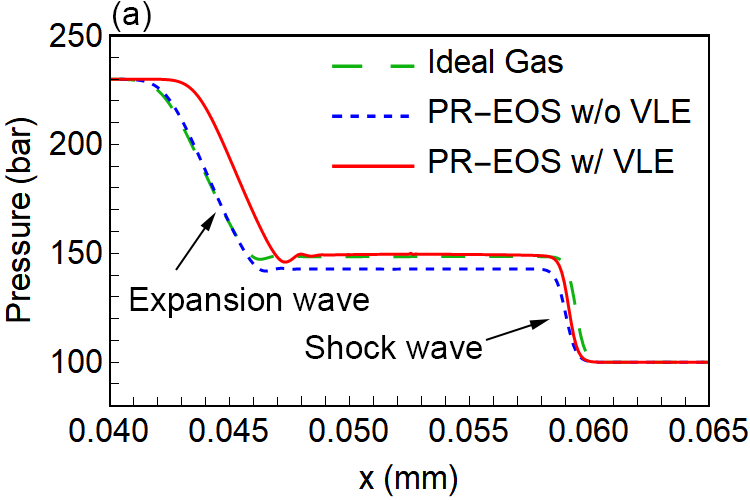
\includegraphics[width=0.45\linewidth]{shock_tube_p.png}
            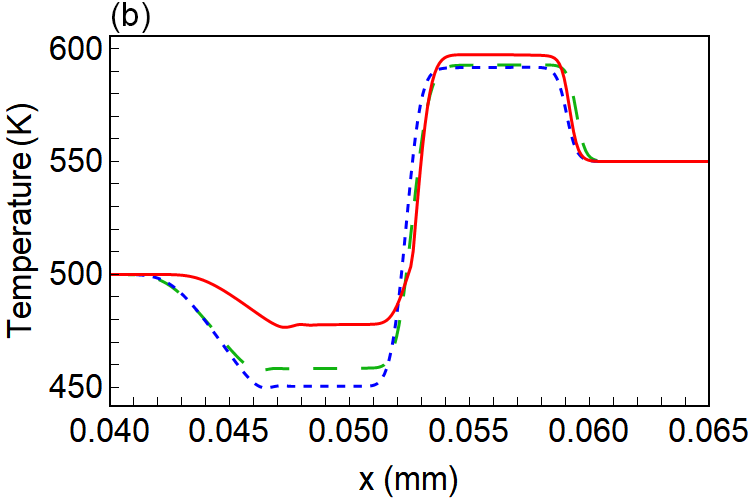
\includegraphics[width=0.45\linewidth]{shock_tube_T.png}
            %\caption{fig1}
        \end{minipage}%
    }\\
    %#\subfigure{\begin{minipage}[t]{1\linewidth}
    %\centering
    %\includegraphics[width=1.5in]{st/stt1.png}
    %\caption{fig2}
    %\end{minipage}%
    %}
    \subfigure{
        \begin{minipage}[t]{1\linewidth}
            \centering
            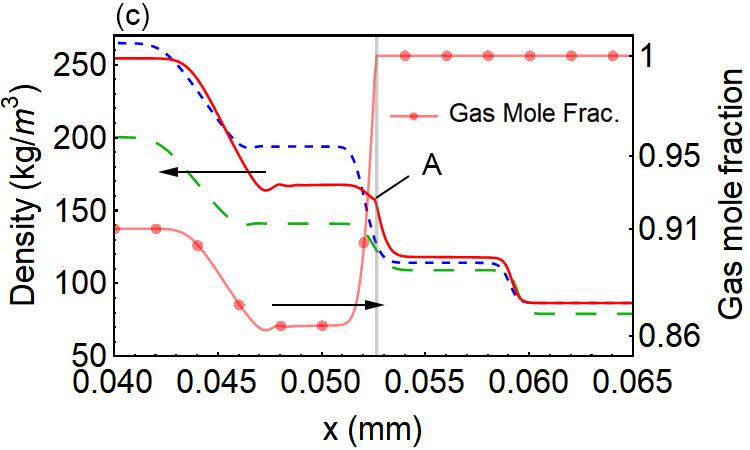
\includegraphics[width=0.50\linewidth]{shock_tube_rho.png}
            %\caption{fig2}
        \end{minipage}%
    }%
    %\subfigure{
    %\begin{minipage}[t]{1\linewidth}
    %\centering
    %\includegraphics[width=2in]{st/stvf_rho.png}
    %\caption{fig2}
    %\end{minipage}%
    %}%
    \caption{Simulation results of a shock tube with \ce{CO2}/\ce{H2O} mixture, at $t=2\times10^{-8}s$: (a) pressure; (b) temperature; (c) density and gas mole fraction.}
    \label{v9}
\end{figure}

To show the importance of real-fluid EOS and VLE models in CFD simulations, three models are used and compared:
\begin{itemize}
    \item ideal gas model;
    \item real-fluid model (PR-EOS) without phase change (i.e., without VLE);
    \item real-fluid model (PR-EOS) with phase change (i.e., with VLE).
\end{itemize} %( From Fig.\ref{v9}, expansion wave speed of phase change result is smaller which is caused by the different sound speed of liquid mixture.)
From the pressure plot in Fig.~\ref{v9}(a), it is apparent that the expansion wave in the PR-EOS model with VLE propagates slower, which is due to lower sound speed (with VLE: 312-323 m/s; without VLE: 363-378 m/s. The VLE sound speed is calculated based on the formula in Tudisco and Menon~\cite{tudisco2020analytical}). The phase equilibrium includes thermal equilibrium, mechanical equilibrium, and chemical equilibrium. In an isentropic process (i.e., $dS=0$), when volume decreases (i.e., for a given $dV<0$), these equilibria mitigate the pressure rise to minimize the total energy $E$ and hence minimize the total energy rise $(dE = -pdV + TdS)$. Consequently, with the same $\Delta\rho$, phase equilibrium makes $p$ and hence the pressure rise $\Delta p$ smaller than those without VLE. According to the formula of sounds speed $c=\sqrt{\Big(\frac{\partial p}{\partial \rho}\Big)_s}$, VLE causes the drop of sound speed.
%Specifically, in the isentropic process, at a change in density, the pressure change is reduced by phase change, and hence sound speed $c=\sqrt{\Big(\frac{\partial p}{\partial \rho}\Big)_s}$ is smaller. In contrast, the mixture in the compression shock wave is in a pure gas phase due to the higher temperature. Thus, the shock wave speed is not affected by phase change. %, and the post-compressor mixture should be in a pure gas phase.
In Fig.~\ref{v9}(b), because phase change is taken into account, latent heat is released when vapor partially condenses during the expansion wave propagation, which reduces the temperature reduction and makes PR-EOS with VLE have the highest temperature. In Fig.~\ref{v9}(c), the three models show evident differences in density prediction. Specifically, compared to the real-fluid models (PR-EOS), the ideal gas model underestimates the gas density. The effect of the phase change (i.e., VLE) increases the temperature in the expansion wave and hence reduces the density there. The gas mole fraction, predicted by the real-fluid model with phase change (i.e., with VLE) at different positions, indicates that the mixture is partially condensed after the expansion wave. Also, a sharp bend (point A) in the density line only exists in the prediction from the PR-EOS model with VLE, which corresponds to the location where the mixture starts to condense.

In summary, the real fluid model integrated with VLE can capture more physics caused by phase change. %including: the propagation of expansion waves slows down, and temperature jump is mitigated.
The results show that expansion waves can trigger significant condensation in premixed \ce{sCO2} systems, and the latent heat of the condensation can change the temperature and density fields in the systems. Moreover, the speed of the expansion wave is reduced.
%Note that the effect of the expansion wave is similar to the local flow acceleration near the leading edge of the compressor impeller. The results in Fig.~\ref{v9} show that condensation is likely to happen near the leading edge. The results in Sec.~\ref{thermo analysis} also show that liquid phase could be formed in the compressor due to the effect of multicomponent mixture. The combination of these two causes (i.e., flow acceleration and multicomponent effects) may result in more severe erosion.

%Note that the turbine inlet temperature in real \ce{sCO2} systems are significantly higher than the initial temperature of this shock tube case shown in Table~\ref{conditions}. Thus the expansion process in a \ce{sCO2} turbine is not sufficient to trigger the partial condensation, and a recuperator is necessary to trigger the partial condensation. 



% \subsection{2D LES of the turbulent mixing between \ce{CO2} and \ce{H2O}}
% %In addition to heating/cooling and compression/expansion, a more interesting way to trigger phase change is mixing. 
% Mixing can raise the critical point such that the mixture enters the subcritical two-phase zone without significant changes in temperature and pressure, which is a typical way to trigger phase separation.
% %, a special type of phase change. 
% %Although there is no mixing process in real \ce{sCO2} compressors and turbines, it is still worthy of studying the mixing of \ce{CO2} and \ce{H2O} from a scientific perspective. 
% In this section, a 2D channel flow simulation is conducted to investigate the mixing-driven phase separation. In this simulation, hot \ce{H2O} vapor (590 K) is injected into cold \ce{CO2} (430 K). In the injectors of both \ce{CO2} and \ce{H2O}, the local temperature is higher than its dew point. This means that \ce{CO2} and \ce{H2O} are both in the gas phase, which can be seen from the gas mole fraction plot (Fig.~\ref{v2d1}). After \ce{H2O} is injected into the \ce{CO2}, due to mixing, water vapor is cooled quickly and partially condensed in the channel. The VLE-based CFD solver can capture the phase separation, as indicated by the gas mole fraction change in Fig.~\ref{v2d1}. Note that the mixture temperature is still higher than the dew point of water, so the condensation of water is due to a combined effect of the lower temperature and the mixing. Figure~\ref{v2dp} explains the observation based on the thermodynamic analysis. The thermodynamic states of pure \ce{CO2} and \ce{H2O} are out of the subcritical two-phase zone and in the gas phase. But after the mixing, the dew line of the mixture moves to a higher temperature. The mixture temperature is between the initial temperature of \ce{H2O} and \ce{CO2}, falling into the corresponding subcritical two-phase zone in the phase diagram, and then the condensation happens.
% \begin{table}[htbp]

%     \begin{center}
%         \begin{minipage}{0.9\textwidth}
%             \caption{Inlet conditions of the 2D channel flow of \ce{CO2}/\ce{H2O} mixture.}\label{conditions2}
%             \begin{tabular}{@{}lllll@{}} %\hline
%                 \toprule
%                          & $P$ (bar) & $T$ (K) & $u_{\rm{inlet}}$ (m/s) & $\rm{width}_{\rm{inlet}}$ (mm) \\ %\hline
%                 \midrule
%                 \ce{CO2} & 100       & 430     & 1                      & 7                              \\ %\hline
%                 \ce{H2O} & 100       & 590     & 10                     & 10                             \\ %\hline
%                 \bottomrule
%             \end{tabular}
%         \end{minipage}
%     \end{center}

% \end{table}

% \begin{figure}[htb]
%     \centering
%     %\begin{minipage}[t]{0.5\linewidth}
%     \centering
%     \subfigure{
%         \begin{minipage}[t]{0.8\linewidth}
%             \centering
%             \includegraphics[width=0.9\linewidth]{channel_flow_result.png}
%             %\caption{fig2}
%         \end{minipage}%
%     }
%     %\end{minipage}%
%     \caption{Schematic and instantaneous temperature, \ce{H2O} mole fraction, and gas mole fraction of the 2D channel flow of \ce{CO2}/\ce{H2O} mixture.}
%     \label{v2d1}
% \end{figure}

% \begin{figure}[htbp]
%     \centering
%     %\begin{minipage}[t]{0.5\linewidth}
%     \centering
%     \subfigure{
%         \begin{minipage}[t]{1\linewidth}
%             \centering
%             \includegraphics[width=0.5\linewidth]{channel_flow_phase_diagram.png}
%             %\caption{fig2}
%         \end{minipage}%
%     }
%     %\end{minipage}%
%     \caption{Temperature-pressure phase diagram of the 2D channel flow of \ce{CO2}/\ce{H2O} mixture at different \ce{CO2} mass fraction values.}
%     \label{v2dp}
% \end{figure}


%\subsection{Mixture critical point and phase separation at conditions relevant to \ce{sCO2} oxy-combustors}
%\label{sec:result:combustor}

%In \ce{sCO2} oxy-combustors, \ce{CH4} and \ce{O2} are injected through nozzles. The temperatures of \ce{CH4} and \ce{O2} are relatively lower than the ambient temperature, which might be cold enough to let the small amount of \ce{H2O} in the working fluid (a \ce{CO2}/\ce{H2O} mixture) condense. Hence, phase separation might occur near the injectors of fuel and oxidizer. The supercritical mixture is partially condensed into small liquid droplets, which could affect the cold ignition in \ce{sCO2} oxy-combustors. Specifically, the ``effective" ignition delay could be enlarged due to the phase change processes. In addition, it might also lead to combustion-induced Rapid Phase Transition (cRPT) \citep{basco2013effect}, which causes anomalous high or oscillating pressures and may damage the equipment and cause safety issues. In this section, the mixing and phase separation are investigated at conditions relevant to \ce{sCO2} oxy-combustors.



%\subsubsection{Subcritical and supercritical mixing in \ce{sCO2} oxy-combustors: jet-in-crossflow simulations} 
\subsection{3D LES of turbulent jet-in-crossflows in the \ce{sCO2} systems: mixing-driven phase separation}
\label{sec:results:JICF}
To understand the mixing-driven phase separation in the \ce{sCO2} systems (e.g., the fuel and oxidizer injections in \ce{sCO2} oxy-combustors), large-eddy simulations (LES) of turbulent jet-in-crossflows are conducted. As shown in Appendix~\ref{App:vali:CFD}, the CFD solver based on the PIMPLE algorithm has been validated by another turbulent jet-in-crossflow case. %\comment{In the current case, pure \ce{O2} and \ce{CH4} are used to represent the oxidizer and fuel, respectively.}
In each simulation, cold (300 K) \ce{O2} or \ce{CH4} is injected from the nozzle at the bottom into hot (500 K or 700 K) \ce{CO2} which contains a small amount of \ce{H2O} (10\% or 20\%). %\comment{to represent the \ce{H2O} generated by the combustion of the last cycle. The existing technology can achieve a \ce{CO2} mole fraction of 96\% in the \ce{sCO2} oxy-combustor \cite{mcclung2015high}. The mole fraction of \ce{H2O} can be 4\% or larger. Here, exaggerated values of 20\% and 10\% \ce{H2O} are used for simulation to show phase separation better.} 

Auto-ignition simulations at a constant pressure of 300 bar are conducted using Cantera~\cite{goodwin2009cantera} with GRI-Mech 3.0 \cite{smith1999gri} as the chemical mechanism. Figure~\ref{JICFautoig} shows that at 700 K the ignition delay is about 20 s, but the time scales of the mixing and phase separation processes of the jet-in-crossflow in this study are less than 1 ms. Moreover, the injected \ce{O2} and \ce{CH4} are at 300 K, which makes it difficult to have any obvious chemical effect. For these reasons, chemical reactions do not need to be considered at the conditions of this study.

More details about settings, geometry, and mesh are shown in Table~\ref{JICFconditions} and Fig.~\ref{JICFg}. 
The mesh in the simulation contains 17.5M cells in total. The integral length scale $l_0$ is estimated using a Reynolds-averaged Navier–Stokes (RANS) simulation. $l_0\approx24 \rm{\mu m}$ in the interested region (0.4 cm $< x <$ 1.5 cm). The mesh in the interested region is refined to make sure $\Delta<l_0/5$, where $\Delta$ is the grid size and $\Delta \approx 3 \rm{\mu m}$. When the above condition is satisfied, about 80\% turbulent kinetic energy can be resolved by the mesh (the well-accepted criterion for LES resolution) \cite{gerasimov2016quick}, and hence the mesh resolution is high enough for LES \cite{pope2004ten}. Subgrid-scale (SGS) stress tensor is evaluated using the Smagorinsky model~\cite{smagorinsky1963general}.  Since the VLE-based CFD of high-pressure multiphase flows is relatively new (more precisely, less than a decade), there is no investigation on the SGS mixing models of filtered VLE equations. Even the SGS mixing models for filtered real-fluid EOS are still not mature~\cite{unnikrishnan2017subgrid,unnikrishnan2021subgrid}. %These models are necessary for the LES prediction of transcritical fluid flows, and hence need to be better investigated. 
In this work, due to the limitations of the state-of-the-art, we do not consider the SGS terms of filtered VLE equations and filtered real-fluid EOS but will investigate them in the future. % and only qualitatively investigate the mixing and phase separation in \ce{sCO2} gas turbine systems.} 

\begin{table}[htb]

    
    \begin{minipage}{0.9\textwidth}
        \caption{Injection nozzle and inflow conditions of the turbulent jet-in-crossflows.}    \label{JICFconditions}

        \begin{center}
            \begin{tabular}{@{}lllll@{}}% \hline
                \toprule
                $p$ (bar) & $T_{\rm{nozzle}}$ (K) & $T_{\rm{inflow}}$ (K) & $U_{\rm{nozzle}}$ (m/s) & $x_{\ce{H2O}}$ \\ %\hline
                \midrule
                300       & 300                   & 500 or 700            & 300                     & 0.2 or 0.1     \\%\hline
                \bottomrule
            \end{tabular}
        \end{center}
    \end{minipage}

\end{table}
\begin{figure}[htb]
    \centering
    \subfigure{
        \centering
        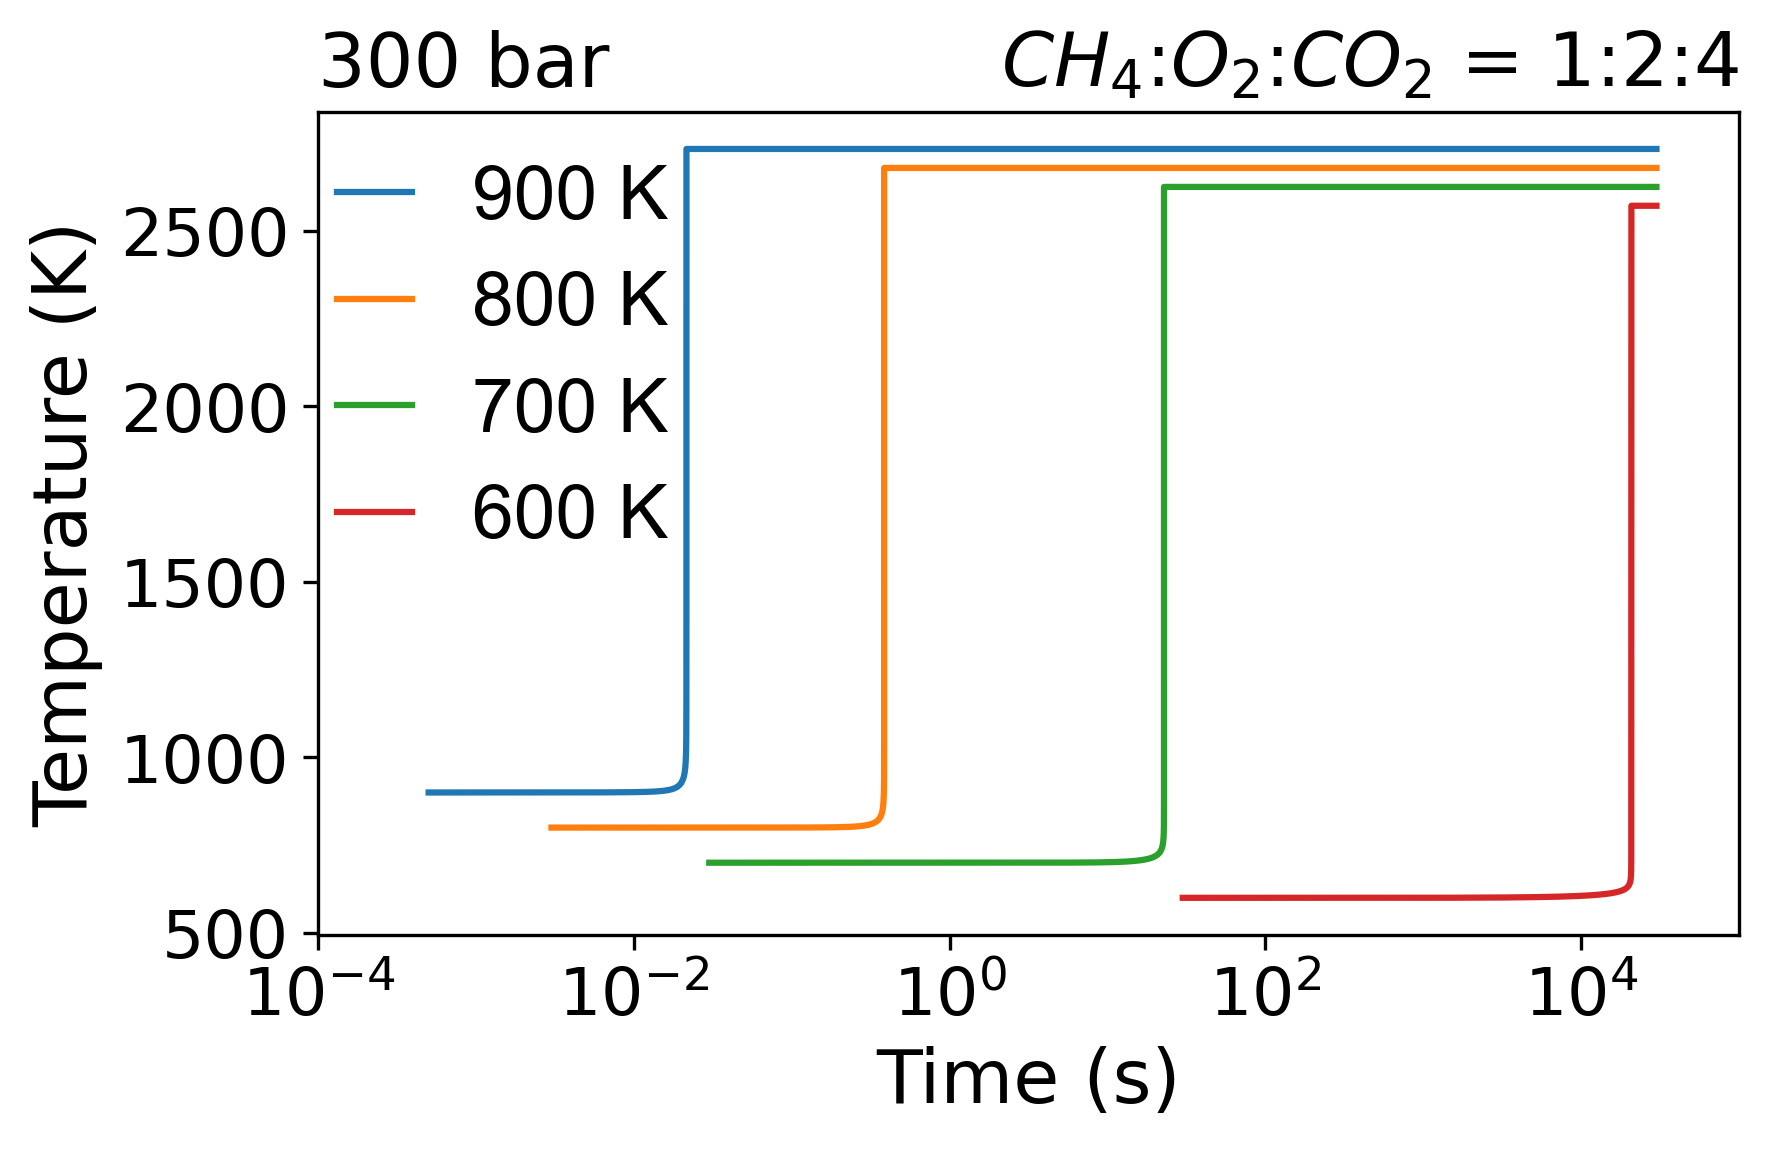
\includegraphics[width=0.6\linewidth]{autoig.png}
    }
    \caption{Temperature vs. Time plot: auto-ignition of \ce{CH4}/\ce{O2}/\ce{CO2} system at a constant pressure of 300 bar. \ce{CH4}:\ce{O2}:\ce{CO2} = 1:2:4, by mole.}
    \label{JICFautoig}
\end{figure}
\begin{figure}[htb]
    \centering
    \subfigure{
        \centering
        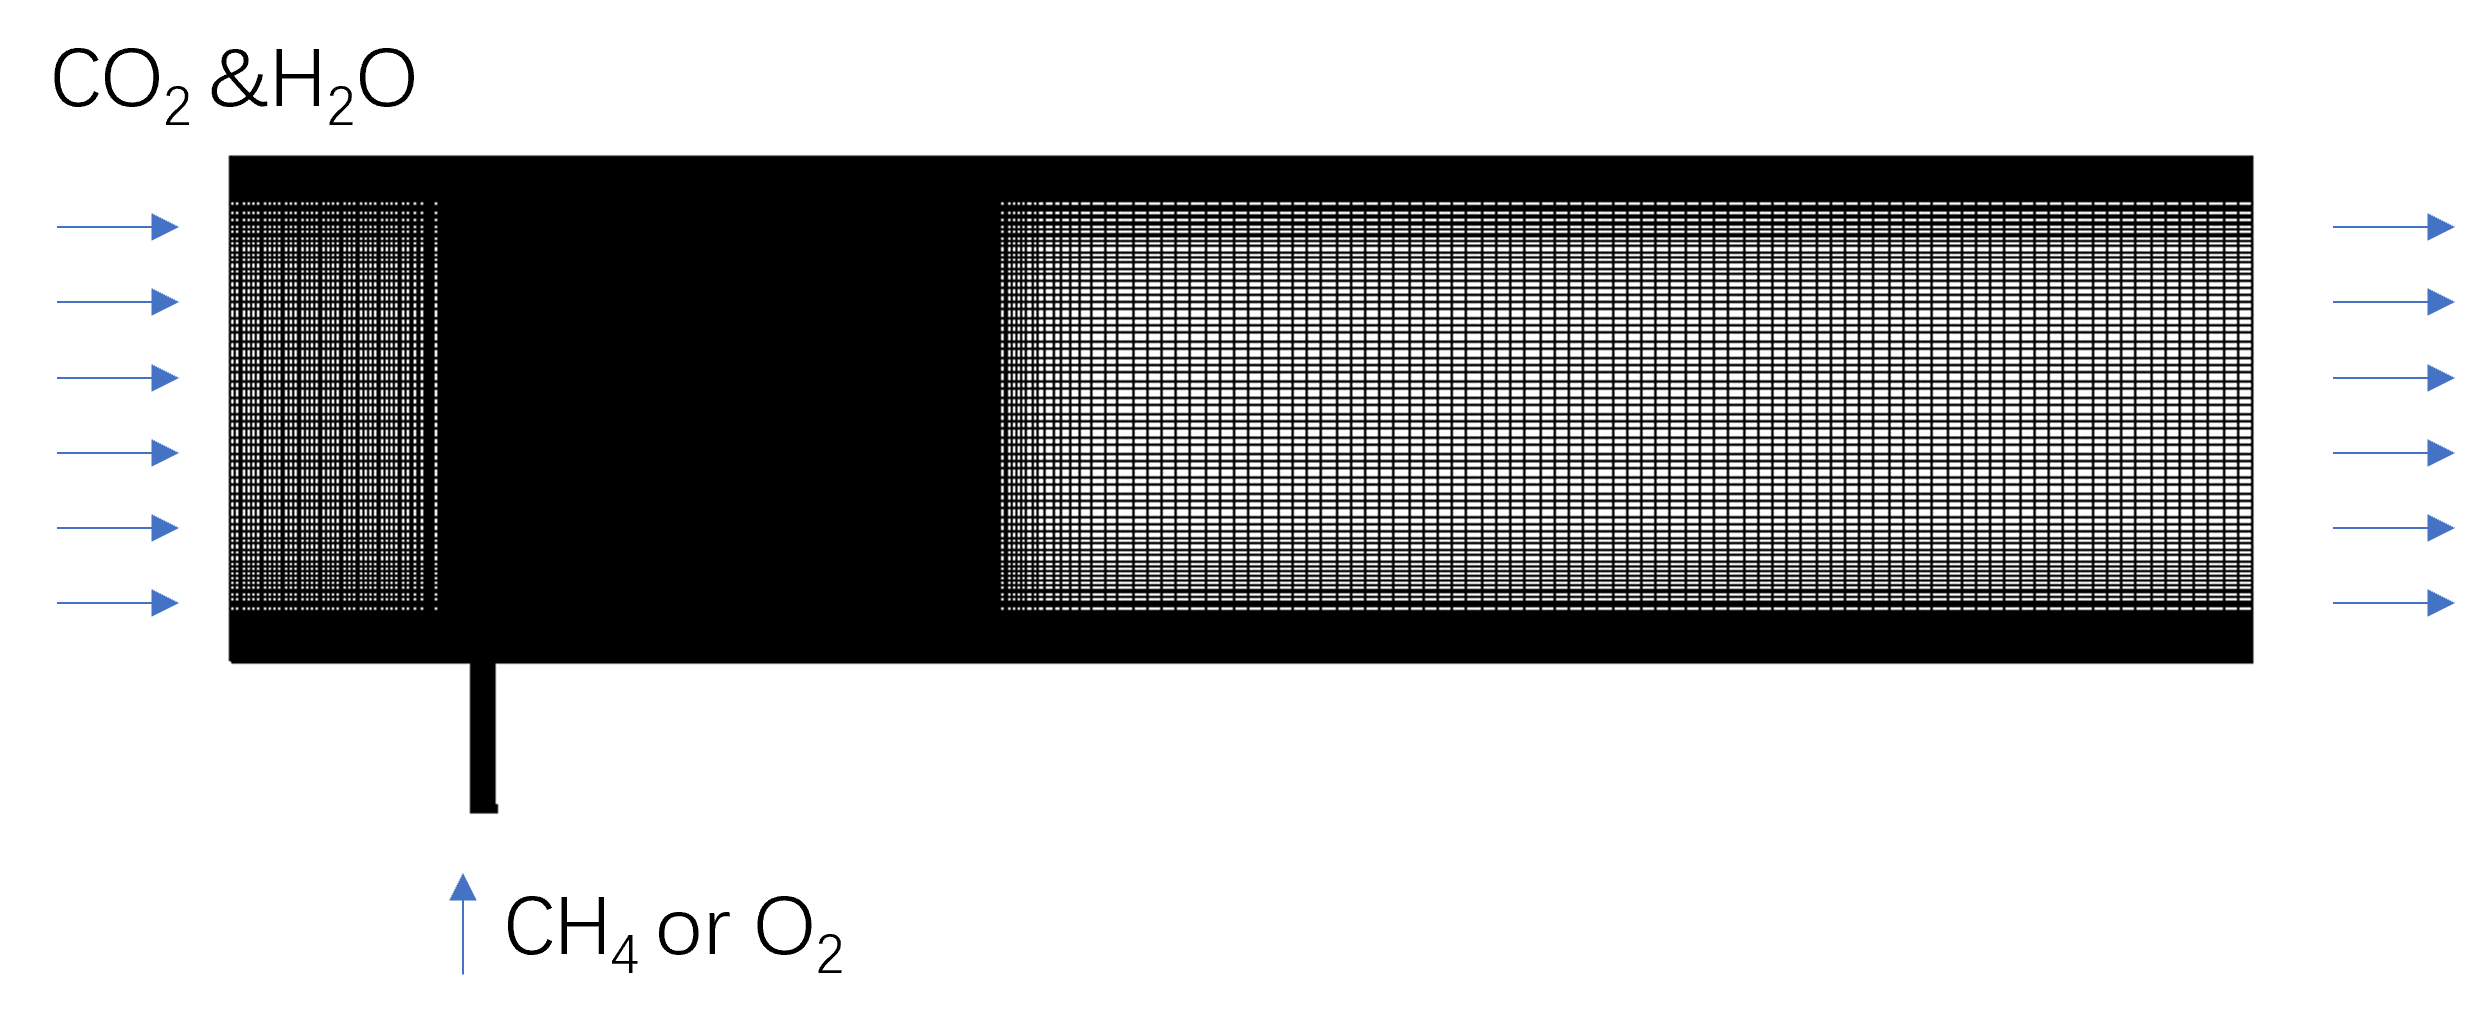
\includegraphics[width=0.6\linewidth]{fg2.png}
        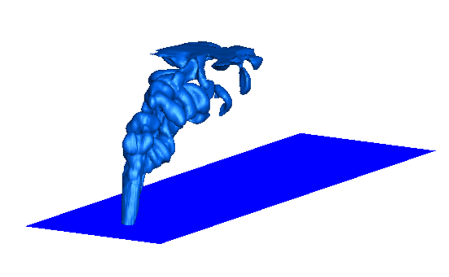
\includegraphics[width=0.4\linewidth]{JICF_schematic.png}
    }
    \caption{Computational mesh and geometry of the turbulent jet-in-crossflows, and iso-suface of \ce{CO2} mole fraction.}
    \label{JICFg}
\end{figure}

Figure~\ref{JICFr}(a-c) shows the results of \ce{O2} injection case. Near the injection nozzle, the cold \ce{O2} is mixed with the hot \ce{CO2}/\ce{H2O} mixture: \ce{O2} concentration keeps high as shown in Fig.~\ref{JICFr}(a), and temperature keeps low as shown in Fig.~\ref{JICFr}(b). In almost the same region, phase separation occurs as shown in Fig.~\ref{JICFr}(c). The cold \ce{O2} is in a supercritical gas-like state, and the hot \ce{CO2}/\ce{H2O} mixture is in the gas phase before they are mixed. However, the temperature of the injected \ce{O2} is low enough to let the gaseous \ce{H2O} in the working medium (i.e., the \ce{CO2}/\ce{H2O} mixture) partially condense (i.e., the mixture enters the subcritical two-phase zone). %After injecting \ce{O2} into the domain, the mixing process reduces the temperature of the mixture containing \ce{H2O}, and then the mixture partially condensed. 
With the mixing process proceeding, the low-temperature \ce{O2} is diluted, and the mixture temperature goes up to the initial temperature of the \ce{CO2}/\ce{H2O} mixture (i.e., the ambient temperature). The small amount of \ce{H2O} in liquid phase quickly evaporate back to the gas phase. Hence, phase separation only appears near the injection nozzle, which agrees with the 0D thermodynamics analysis in Sec.~\ref{sec:results:combustor:H2O}. A similar phenomenon is also observed in the \ce{CH4} injection case, as shown in Fig.~\ref{JICFr}(d).  with Fig.~\ref{JICFr}(d), the jet in Fig.~\ref{JICFr}(c) bends less, and has stronger breakup, which is due to different density ratio $r=\rho_{jet}/\rho_{\infty}$ where $\rho_{\infty}$ is the density of the working medium (i.e., the \ce{CO2}/\ce{H2O} mixture) and $\rho_{jet}$ is the density of the jet fluid from the injection nozzle. \ce{O2} jet has higher density ratio ($r=1.39$ from the data) than \ce{CH4} jet ($r=0.66$ from the data). The jet with higher density ratio trigger stronger breakup, which was also reported in Rachford et al.~\cite{tretola2021effect}.

\begin{figure}[htb]
    \centering
    \subfigure{
        \centering
        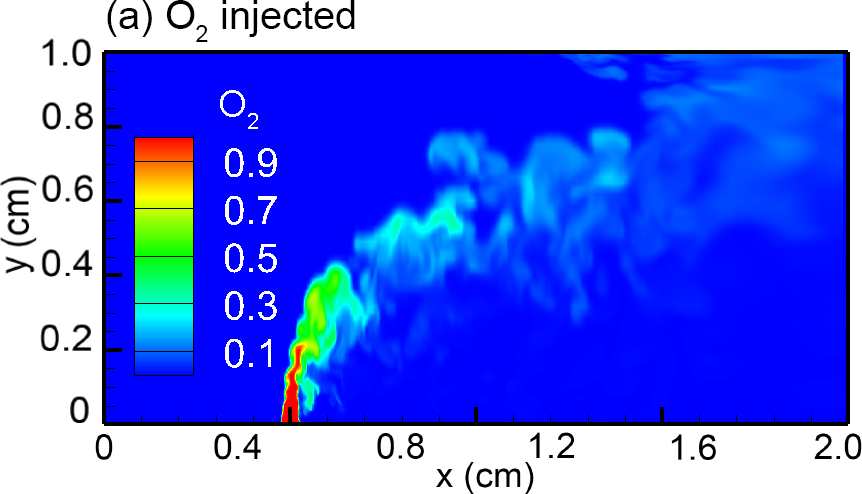
\includegraphics[width=0.45\linewidth]{1a_ps.png}
        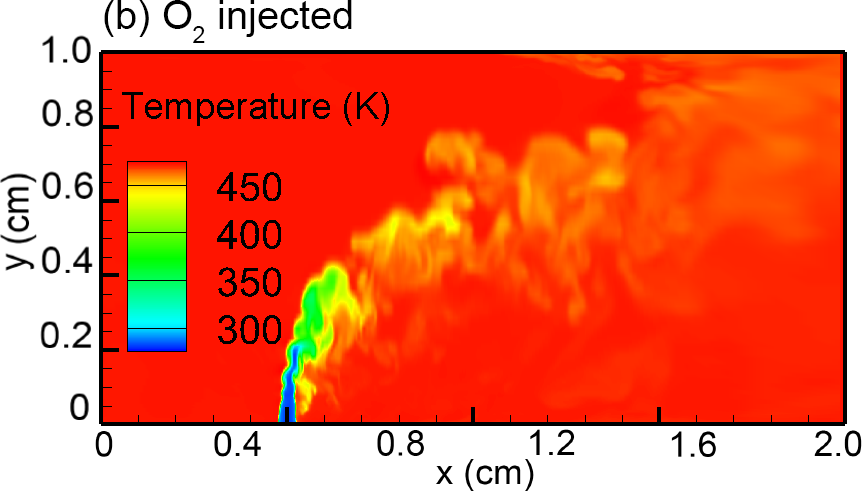
\includegraphics[width=0.45\linewidth]{1b_ps.png}
    }

    \subfigure{
        \centering
        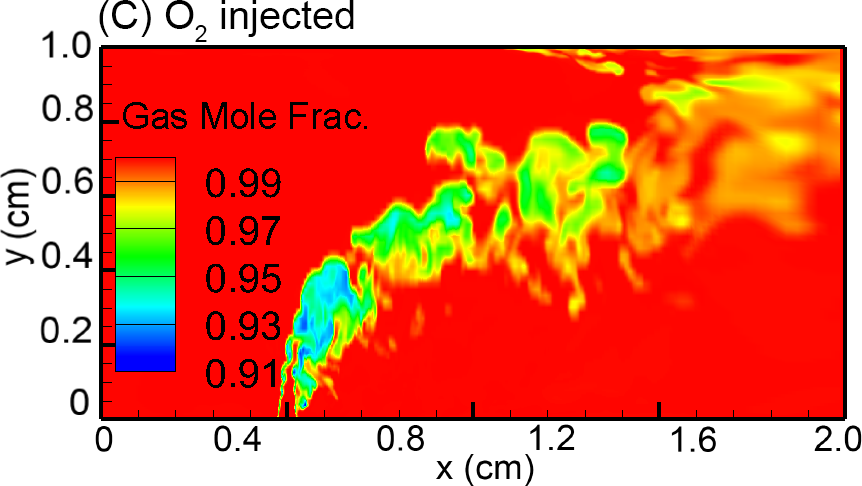
\includegraphics[width=0.45\linewidth]{1c_ps.png}
        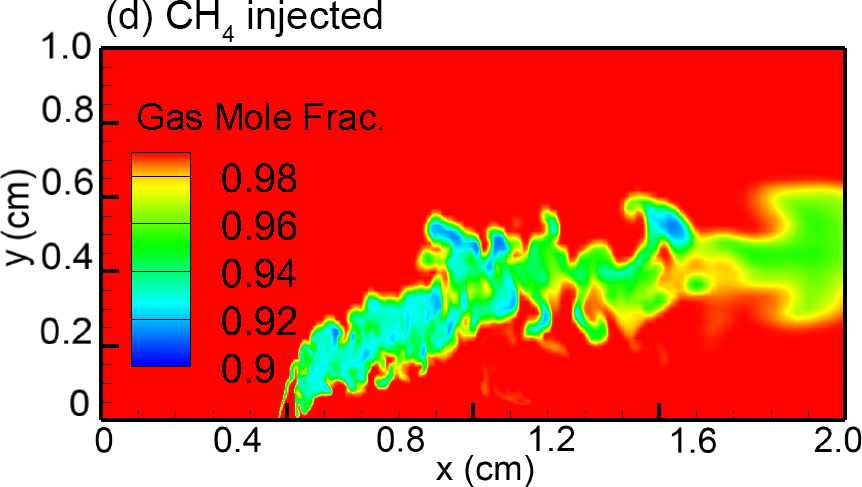
\includegraphics[width=0.45\linewidth]{1d_ps.png}
    }
    \caption{LES of turbulent jet-in-crossflows (ambient temperature is 500 K, and the \ce{CO2}/\ce{H2O} mixture has 20\% \ce{H2O}): (a) mole fraction of \ce{O2} (\ce{O2} is injected); (b) mixture temperature (\ce{O2} is injected); (c) mole fraction of vapor (gas) phase (\ce{O2} is injected); (d) mole fraction of vapor (gas) phase (\ce{CH4} is injected).}
    \label{JICFr}
\end{figure}

It is worth noting that the phase separation condition is sensitive to the variation of ambient temperature. Here, two more simulations for both \ce{CH4} and \ce{O2} injections are conducted at 700 K ambient temperature. The gas fraction distributions of both cases are shown in Fig.~\ref{JICF700}. The phase separation phenomenon becomes much weaker in these two cases: the phase separation region and its gas mole fraction become much smaller. As a result, only a small portion of the mixture condenses and quickly evaporates back to the gas phase.

\begin{figure}[htb]
    \centering
    \subfigure{
        \centering
        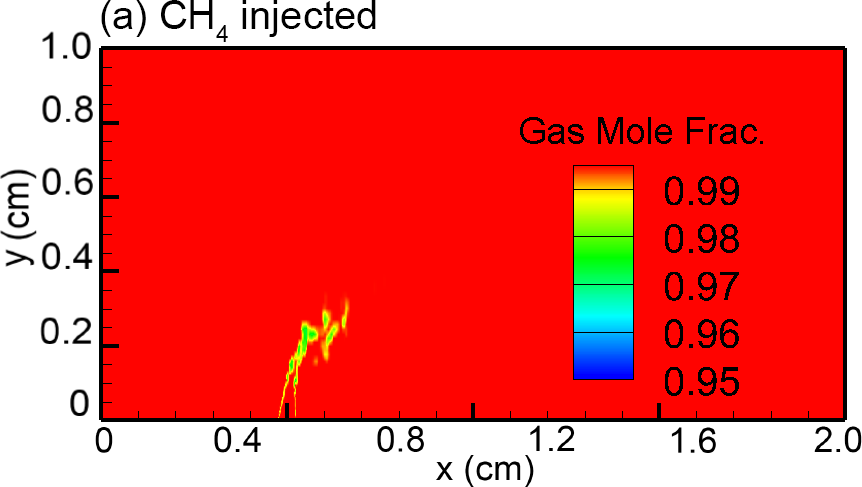
\includegraphics[width=0.45\linewidth]{2a_ps.png}
        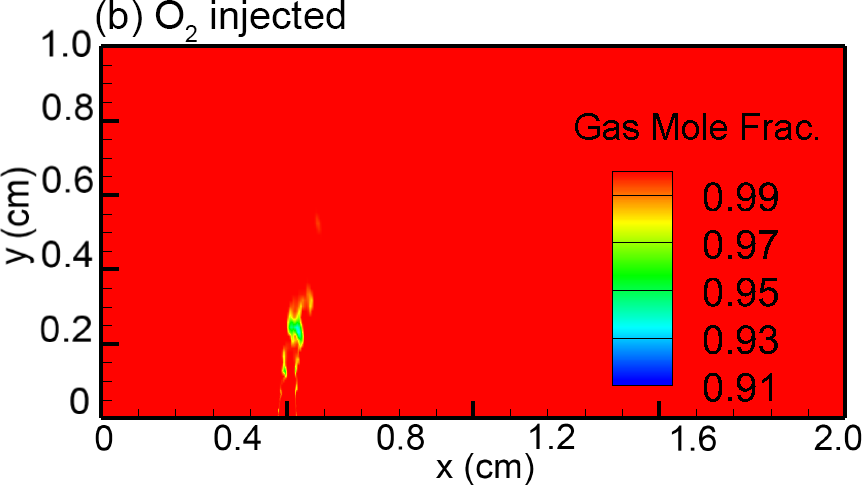
\includegraphics[width=0.45\linewidth]{2b_ps.png}
    }
    \caption{LES of turbulent jet-in-crossflows (ambient temperature is 700K, the \ce{CO2}/\ce{H2O} mixture has 20\% \ce{H2O}): (a) \ce{CH4} is injected; (b) \ce{O2} is injected.}
    \label{JICF700}
\end{figure}

A better understanding of the mixing process and the influence of temperature can be obtained by the thermodynamics analysis of the LES data. In Fig.~\ref{JICFT}, subcritical two-phase and gas-phase regions are colored grey and white, respectively. The phase boundary shown in the plot is at 300 bar. Although the pressure varies in the flow field, the range (289 - 307 bar) is relatively small, which has almost no effect on phase boundaries, as shown in Fig.~\ref{JICFTX}. Hence the phase boundary at 300 bar is a good representation of the boundaries of the system.  The dots are the local thermodynamic states encountered in the LES, which form a curve (i.e., mixing trajectory) to connect the thermodynamic states of the injected fluid and the ambient \ce{CO2}/\ce{H2O} mixture. Since the dew point of \ce{CO2} mixed with 20\% \ce{H2O} is about 500 K, when the ambient temperature is 500 K, the mixing trajectory (green dots) is almost entirely inside the subcritical two-phase zone. When the ambient temperature increases to 700 K, one end of the trajectory of thermodynamic states moves upward, which can be seen clearly from the red dots in Fig.~\ref{JICFT}. As a result, only a small portion of the curve stays inside the subcritical two-phase zone, and phase separation can be observed only in a small region. The isenthalpic mixing lines are also marked in Fig.~\ref{JICFT} to compare with the actual mixing trajectories. The difference between \ce{CH4} injection and \ce{O2} injection can be seen from the comparison between Fig.~\ref{JICFT}(a) and Fig.~\ref{JICFT}(b). For the scenarios with \ce{CH4} injection (Fig.~\ref{JICFT}(a)), at 500 K ambient temperature, the actual mixing trajectories almost overlaps with the isenthalpic lines, which is caused by weak thermal conduction; but at 700 K ambient temperature, larger temperature difference trigger stronger thermal conduction to raise the temperature, and hence the mixing temperature is mostly higher than the isenthalpic mixing temperature. %For the scenarios with \ce{O2} injection (Fig.~\ref{JICFT}(b)), the flow has strong mass diffusion effect. 
%the strong mass diffusion effect can be seen at 700 K ambient temperature, but the \ce{O2} scenarios have more significant mass diffusion effect, which enhances the thermal conduction of both the hot \ce{CO2}/\ce{H2O} mixture and the cold injected \ce{O2}. 
%Hence, the thermodynamic state points (red and green dots of mixing trajectories) of \ce{O2} scenarios are more dispersed than the \ce{CH4} scenarios. 
Compared with Fig.~\ref{JICFT}(a), the points in Fig.~\ref{JICFT}(b) are more dispersed, which is caused by higher density ratio (i.e., $r_{\ce{O2}}=2.4$ is higher than $r_{\ce{CH4}}=1.2$). Higher density ratio triggers stronger breakup, which enhances thermal conduction. Hence, more points deviate from the isenthalpic line.
Although the properties of \ce{CH4} and \ce{O2} affect the dispersion of thermodynamic state points, they do not significantly affect the phase boundaries and the area of the phase separation region in the physical space.

\begin{figure}[htb]
    \centering
    \subfigure{
        \centering
        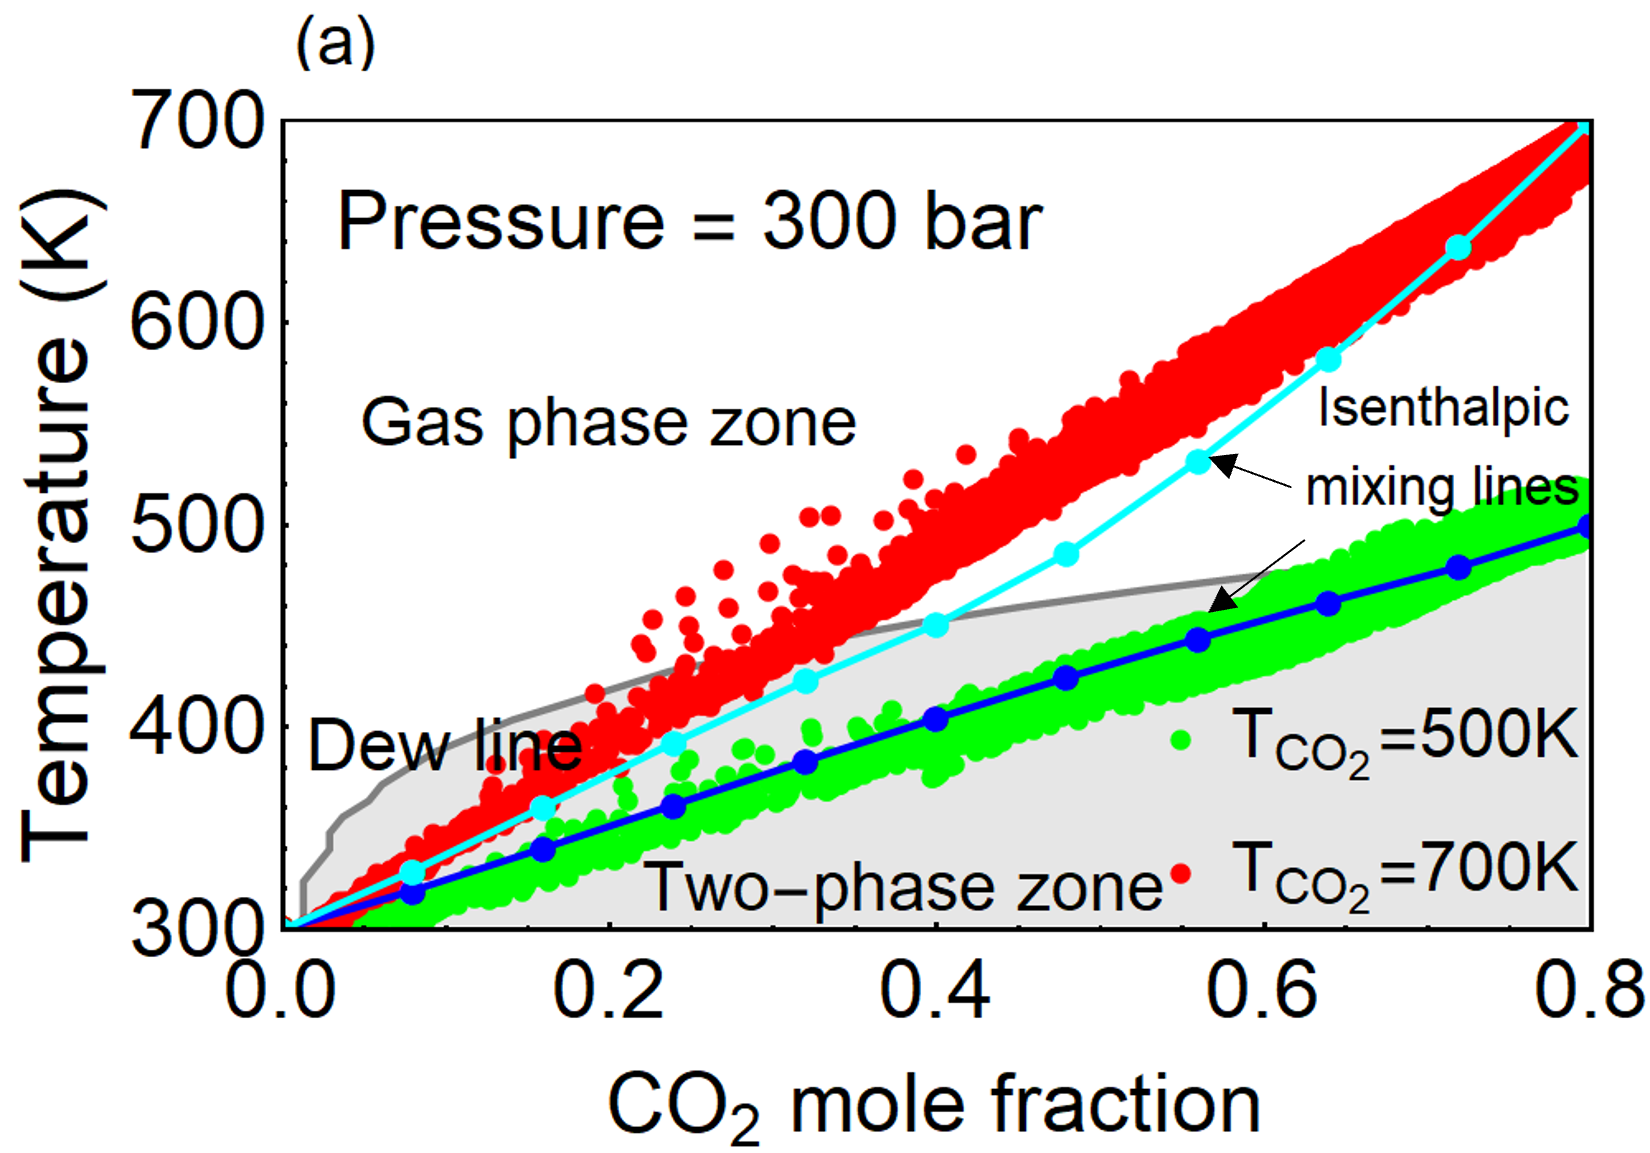
\includegraphics[width=0.45\linewidth]{Ccf_n_u_v2_flow_c.png}
        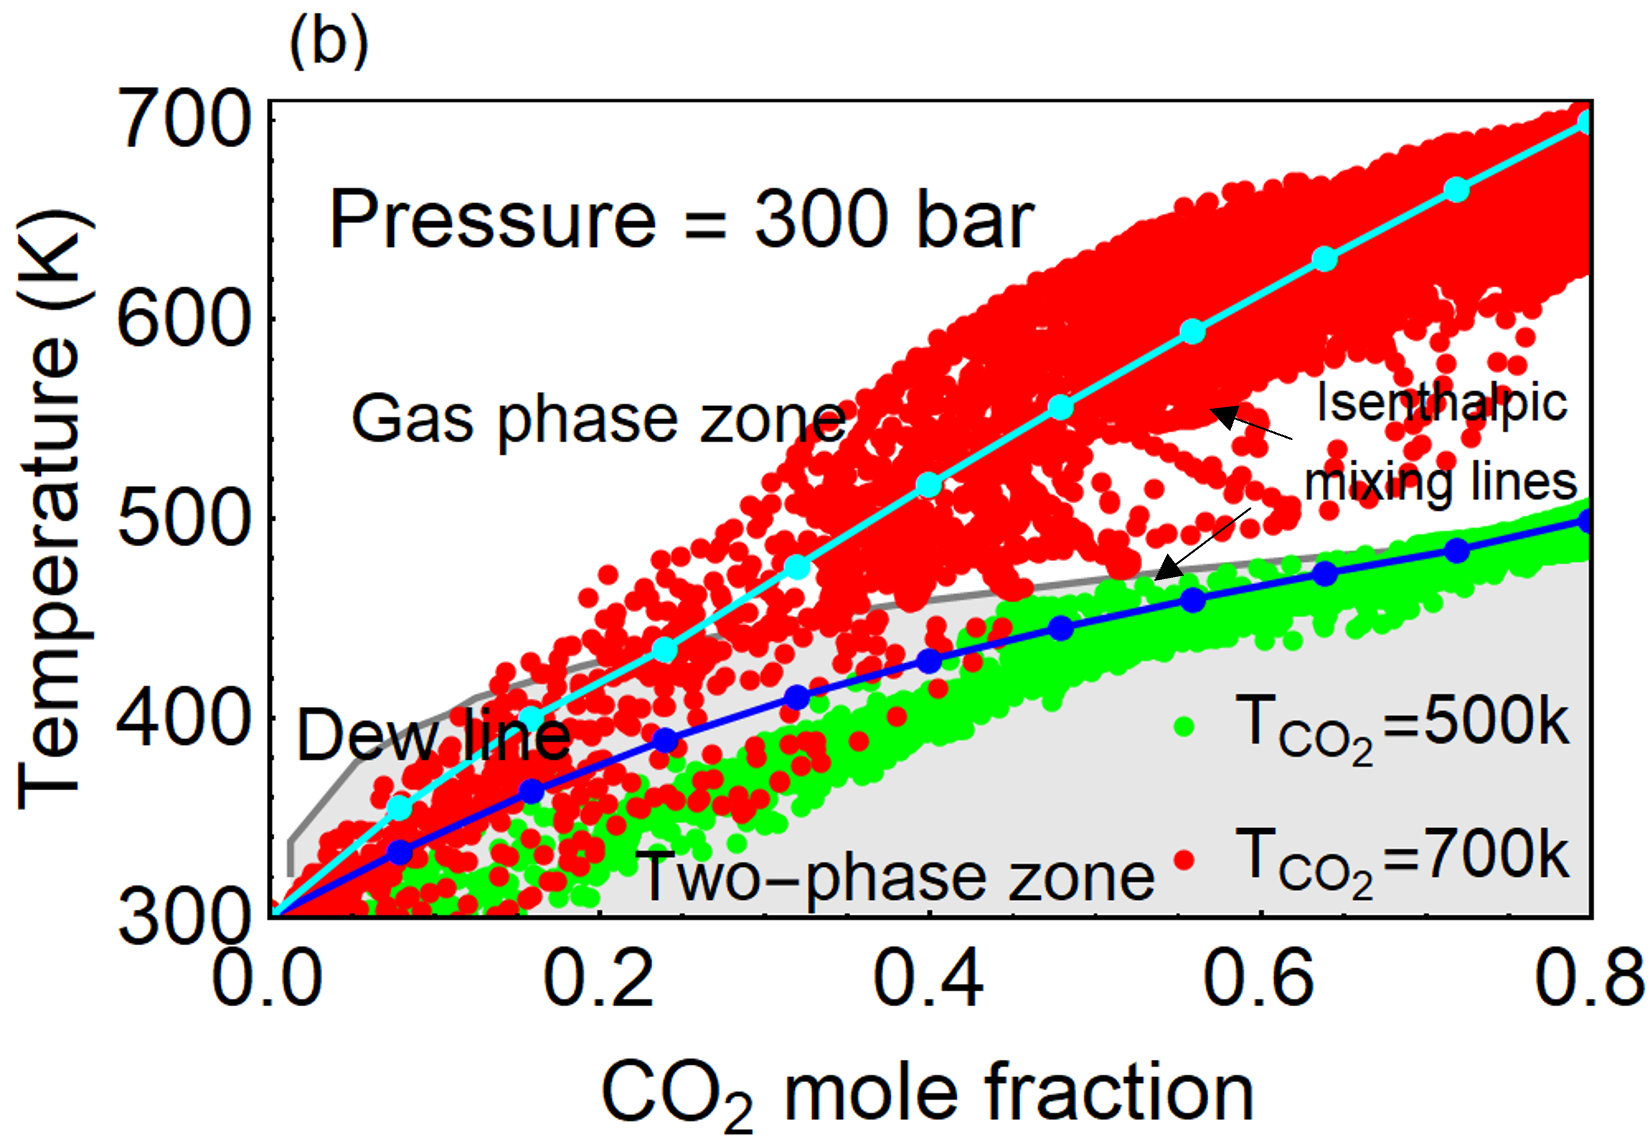
\includegraphics[width=0.45\linewidth]{Cof_n_u_v2_flow_c.png}
    }
    \caption{Temperature-component diagrams of the LES data of two jet-in-crossflows: (a) injecting \ce{CH4} into the \ce{CO2}/\ce{H2O} mixture with 20\% \ce{H2O}; (b) injecting \ce{O2} into the \ce{CO2}/\ce{H2O} mixture with 20\% \ce{H2O}.}
    \label{JICFT}
\end{figure}

\begin{figure}[htb]
    \centering
    \subfigure{
        \centering
        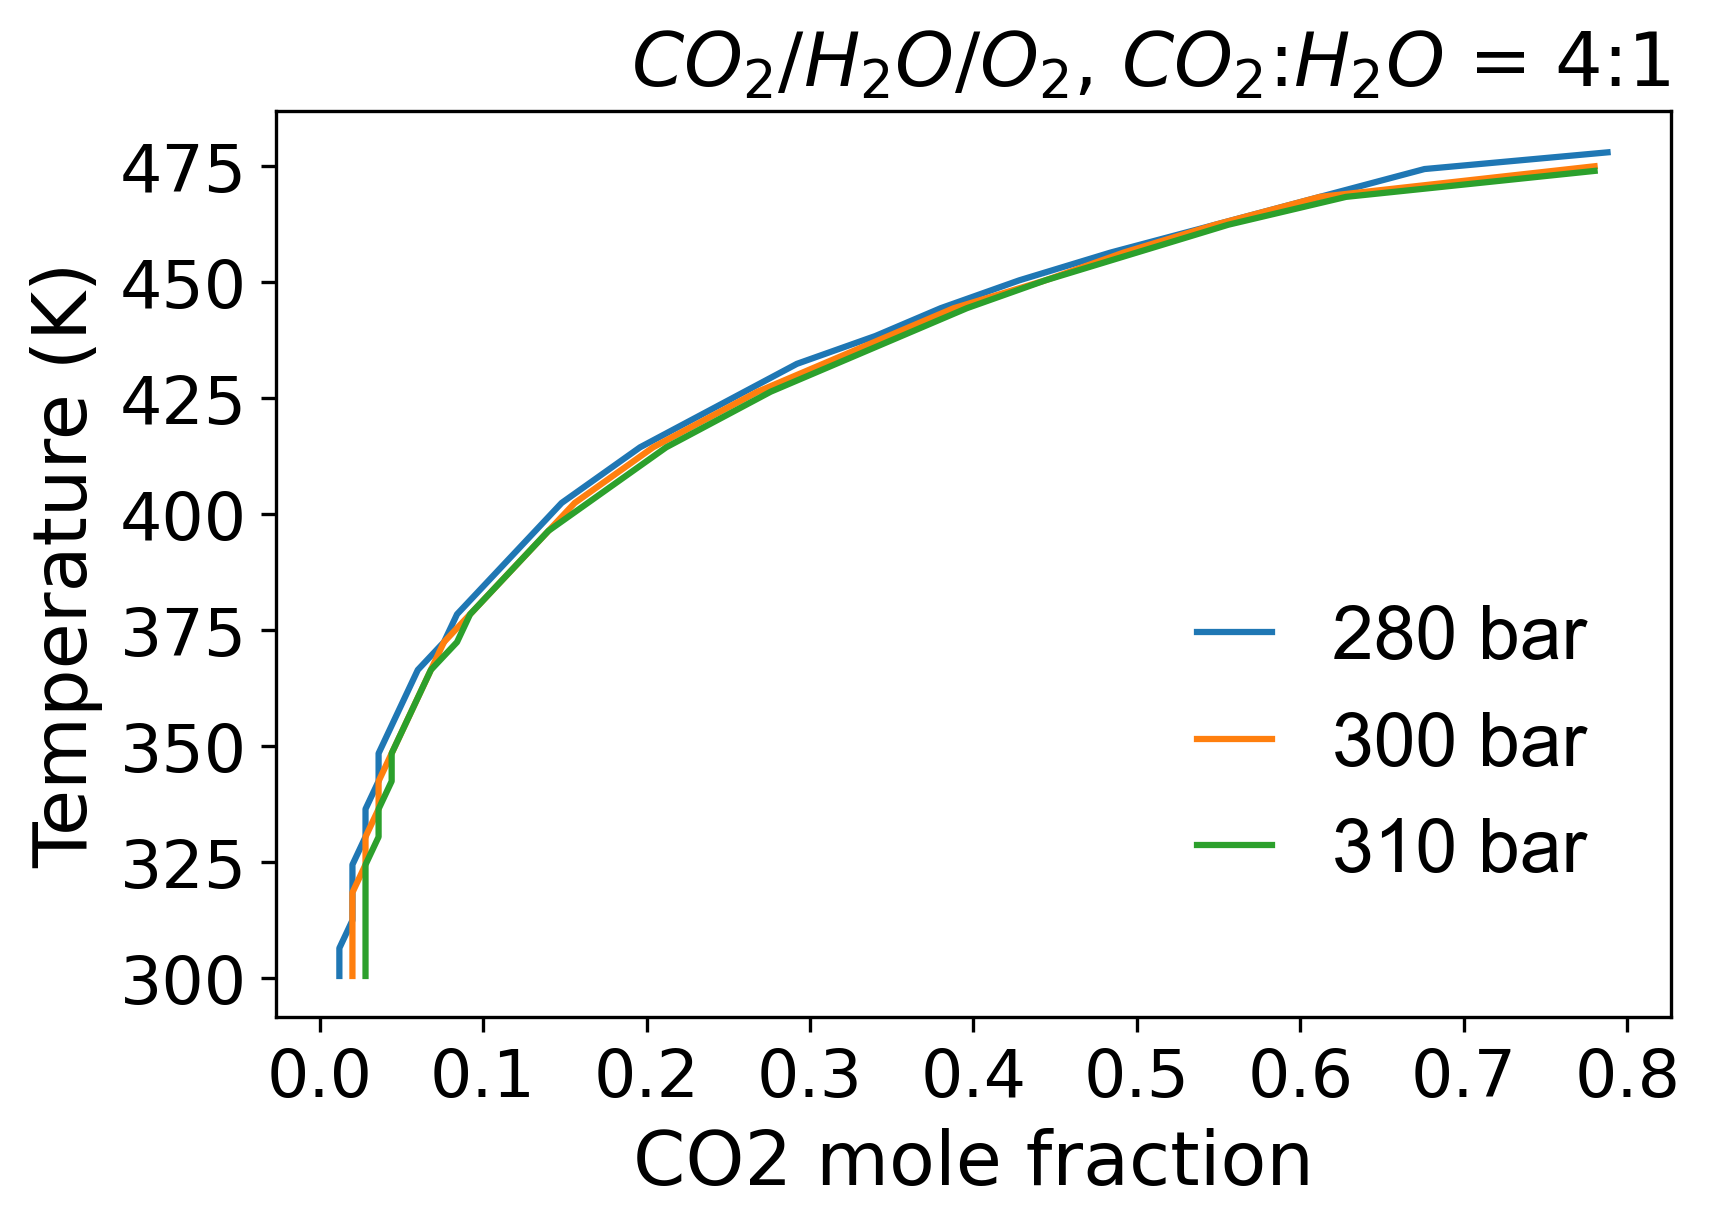
\includegraphics[width=0.45\linewidth]{TX.png}
    }
    \caption{Temperature-component diagrams of a \ce{CO2}/\ce{H2O}/\ce
    {O2} system at 280 bar, 300 bar, 310 bar. \ce{CO2}:\ce{H2O} = 4:1, by mole.}
    \label{JICFTX}
\end{figure}

Finally, the effect of \ce{H2O} addition is investigated. In this case, the ambient temperature is chosen as 500 K, and \ce{CO2} contains 10\% \ce{H2O} instead of 20\% in the previous LES cases. Comparing Fig.~\ref{JICFH}(a) with the previous result in Fig.~\ref{JICFr}(d), less \ce{H2O} leads to a smaller phase separation region. The mechanism behind this can be found in the phase diagram in Fig~\ref{JICFH}(b). The mixing trajectories almost overlap with the isenthalpic lines. The mixture \ce{CO2} with less \ce{H2O} has a lower dew line, and the high-temperature endpoint of the mixing trajectory moves out of the subcritical two-phase zone. The thermodynamic states of most fluid are near that endpoint. Hence, the subcritical two-phase zone in physical space is much smaller than the case with more \ce{H2O}.
\begin{figure}[htb]
    \centering
    \subfigure{
        \centering
        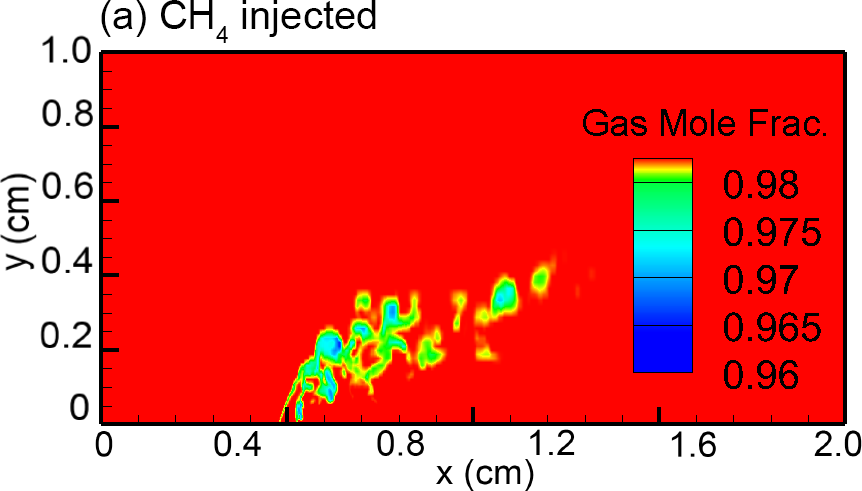
\includegraphics[width=0.5\linewidth]{3a_ps.png}
        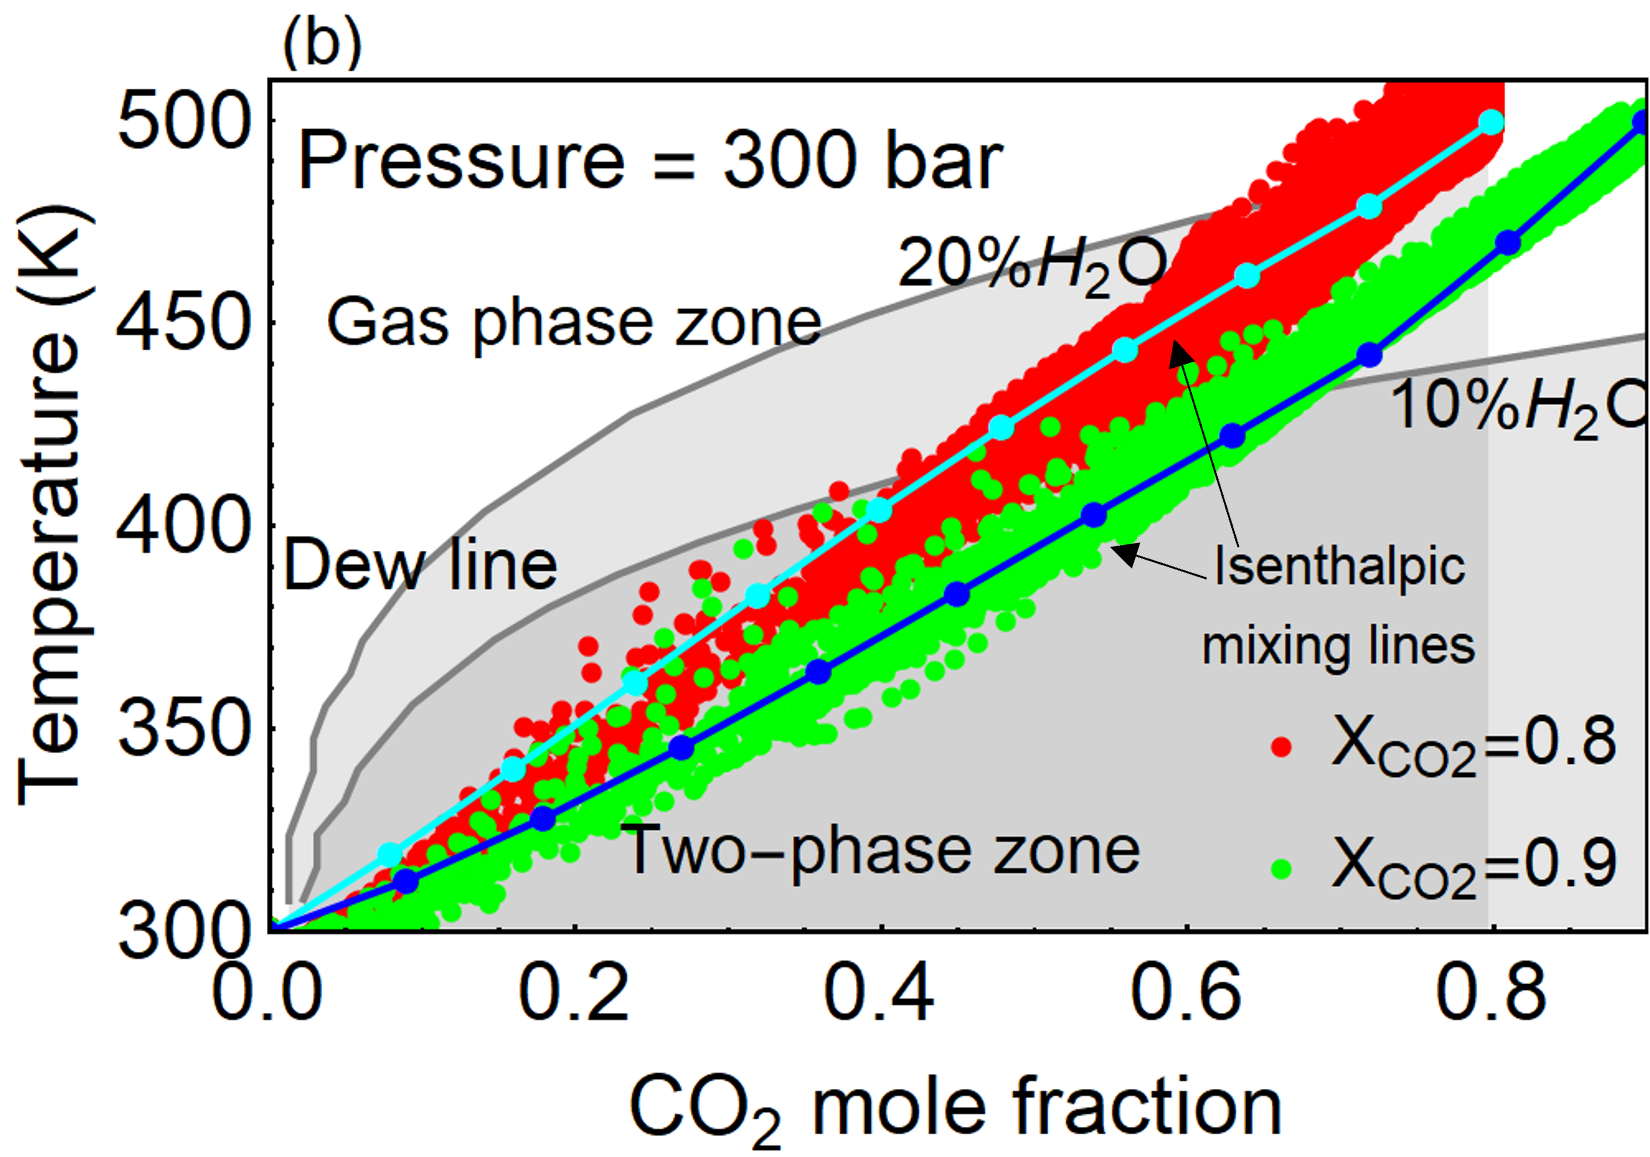
\includegraphics[width=0.4\linewidth]{Chf_n_u_v2_flow_c.png}
    }
    \caption{(a) LES of turbulent jet-in-crossflow of injecting \ce{CH4} into the \ce{CO2}/\ce{H2O} mixture with 10\% \ce{H2O} (ambient temperature is 700 K): (a) gas mole fraction, and (b) temperature-component phase diagram.}
    \label{JICFH}
\end{figure}

The conclusion is that when cold \ce{O2} or \ce{CH4} is injected into a hot mixture of \ce{CO2} and \ce{H2O}, phase separation may occur. This phenomenon requires the \ce{CO2}/\ce{H2O} mixture to be close to the subcritical two-phase zone. %, then distinct phase change can be observed. 
Hence, ambient temperature and \ce{H2O} concentration have an evident influence on the phenomenon. Thermodynamics analysis can only tell whether there is phase separation. In contrast, when the thermodynamics analysis is combined with the CFD simulation, more insights can be obtained about the location and mole fraction of the liquid phase formed during the mixing. %Although the mole fraction of \ce{H2O} is larger than the real working condition, the area of phase separation is small, and the fraction of the liquid phase is not large. Therefore, phase separation may not significantly impact the operation of the combustor at a high temperature. However, at start-up, it could affect the operation. The presence of droplets may increase ``effective'' ignition delay in cold ignition, and the droplets attached to the combustor's inner surface may trigger cRPT~\citep{basco2013effect}, which may damage the equipment and cause safety issues.

%To close the section, although the comparison between the traditional gas turbine combustors and \ce{sCO2} oxy-combustors is not the main focus of this research, the comparison is still important to understand \ce{sCO2} oxy-combustors and hence is performed and presented in~\ref{app:trad}.
%To close the section, although this research mainly focus on the phase separation in \ce{sCO2} system, to understand semi-closed \ce{sCO2} oxy-combustors is still important. Hence, several investigates about the mixture critical points and thermodynamic properties in \ce{sCO2} oxy-combustors are presented in~\ref{app:trad},\ref{thermo analysis}, and \ref{sec:results:combustor:phase}.
%the comparison between the traditional gas turbine combustors and \ce{sCO2} oxy-combustors is not the main focus of this research, the comparison is still important to understand \ce{sCO2} oxy-combustors and hence is performed and presented in~\ref{app:trad}.


\section{Conclusion}
\label{sec:conclusion}
%Power cycles that use direct-fired supercritical \ce{CO2} (\ce{sCO2}) oxy-combustion are attractive for power generations because of their inherent almost 100\% carbon capture, high efficiency, and small machinery footprints. However, the real-fluid thermodynamics of mixture in \ce{sCO2} gas turbine systems are barely explored. 
In this study, the multicomponent effects on the supercritical \ce{CO2} (\ce{sCO2}) systems are investigated.
In order to investigate the multiphase thermodynamics of the \ce{sCO2} systems,
%In order to achieve a better understanding of supercritical \ce{CO2} (\ce{sCO2}) gas turbine systems, 
two vapor-liquid equilibrium (VLE) solvers (i.e., the isothermal-isobaric (TPn) flash solver and isobaric-isenthalpic (HPn) flash solver) are implemented, validated, and verified to predict the phase boundary and real mixture critical point, and simultaneously model the subcritical regime (with the consideration of phase change), the supercritical regime, as well as the transition between them. % (i.e., the transcritical regime). %to conduct thermodynamic calculation and analysis. 
A VLE-based computational fluid dynamics (CFD) simulation framework is also developed by coupling a pressure-based CFD solver with the HPn flash solver to capture the phase separation in high-pressure multiphase flows.
A novel VLE-based tabulation method is developed to make the CFD solver computationally more affordable.
The thermodynamics analyses and CFD simulations are conducted to reveal several mechanisms of phase separation in the \ce{sCO2} systems. %\ce{H2O} addition%\comment{combustion-induced impurity components (i.e., other than \ce{CO2})} 
%on mixture critical points.%\comment{and thermodynamic properties, to capture phase separation in \ce{sCO2} gas turbine systems, and to discuss its possible consequences.} 
The major findings include:
%(TPn flash for isothermal and isobaric processes and HPn flash for isobaric and isenthalpic processes). Also, HPn flash solver is coupled with a computational fluid dynamics (CFD) solver to capture the mixing and phase separation processes of mixtures at conditions relevant to \ce{sCO2} compressors, turbines, and oxy-combustors.

%The TPn flash solver is first validated using the experimental measurement of phase boundary, and then verified by \citet{stradi2001reliable}'s formulization of mixture critical points. The HPn flash solver is verified by \citet{matheis2018multi}'s predictions of equilibrium mixing temperature $T_{eq}$. 

%A thermodynamic analysis is carried out for the multicomponent mixtures in \ce{sCO2} compressors and oxy-combustors under a broad range of temperature and pressure conditions and conducted CFD simulations to capture the detailed mixing and phase separation processes of mixtures at relevant conditions to in \ce{sCO2} compressors, turbines, and oxy-combustors. 
%We firstly report the recommended thermal conditions for the recuperater based on the thermal performance of \ce{sCO2} compressor, in order to achieve the highest thermal efficiency of the system.

\begin{enumerate}
    %\item Mixture critical point:
    %\begin{enumerate}
    \item A small amount of combustion-relevant impurities (e.g., \ce{H2O}, \ce{CH4}, and \ce{O2}) can significantly elevate the mixture critical point of the \ce{sCO2} systems, with a much higher critical pressure than that of each component of the mixture. As a result, the so-called ``supercritical'' \ce{CO2} systems might be in the subcritical two-phase zone where phase separation (e.g., retrograde condensation) occurs. %Specifically, higher \ce{H2O} concentration and lower temperature enhance the phase separation. 
    At the relevant conditions in this study (i.e., 100-300 bar), phase separation only has a small influence on the \ce{CO2/H2O/CH4/O2} mixture density, but has a considerable influence on the heat capacity of the same mixture.
          %\item The addition of \ce{O2} can further increase the mixture critical point.
          %\end{enumerate}

          %\item Potential phase separation:
          %\begin{enumerate}
          %\item Due to the increase of mixture critical point, the thermodynamic states of the \ce{CO2}/\ce{H2O} mixtures at \ce{sCO2} compressor operating conditions could be in subcritical liquid phase. Also, retrograde condensation could occur during the compression process.
    \item For premixed \ce{sCO2} systems (e.g., a premixed \ce{sCO2} shock tube), evident effects of real fluid and phase separation are observed in expansion processes. %The effects are weak in the compression process, but strong in the expansion process. Specifically, 
    Expansion waves can trigger significant condensation in premixed \ce{sCO2} systems and the latent heat of the condensation can change the temperature and density fields in the systems. Moreover, the speed of the expansion wave is reduced by the phase separation.

    \item Even without compression/expansion waves, mixing alone (e.g., in jet-in-crossflows) can raise the critical point such that the mixture can enter the subcritical two-phase zone to trigger phase separation. Specifically, when two subcritical gas or supercritical gas-like streams mix, the mixture can partially condense to subcritical liquid phase.
    %The large-eddy simulations (LES) of jet-in-crossflows provide more insight into the subcritical liquid phase's location and mole fraction formed in the mixing process. 
    Higher pressure, lower temperature, or higher \ce{H2O} concentration can enhance the mixing-driven phase separation phenomenon in the \ce{sCO2} systems. In jet-in-crossflows, \ce{O2} has higher density ratio than \ce{CH4}. Higher density ratio triggers stronger breakup, which enhances thermal conduction. 
    
    %Phase separation only occurs near the injectors of \ce{CH4} and \ce{O2}.%\comment{fuel and oxidizer in \ce{sCO2} oxy-combustors Although the mole fraction of \ce{H2O} is larger than the real working conditions, the area of phase separation is small, and the fraction of subcritical liquid phase is low.}
          %\end{enumerate}

          %\item Without \ce{H2O} addition, the thermodynamic states of mixtures in both traditional gas turbine combustors and \ce{sCO2} oxy-combustors are in gas or gas-like states, and there is no two-phase zone or phase separation. In contrast, even a small amount of \ce{H2O} addition can significantly increase the mixture critical point. A big portion of the \ce{sCO2} oxy-combustor operating conditions overlaps with the two-phase zone to trigger phase separation.

    %       \comment{
    % \item Potential consequences of phase separation:
    %       \begin{enumerate}
    %           \item Close to the critical point of \ce{CO2}, the compressibility of the mixture and the required compression work are still very low to maintain high thermal efficiency, but it is due to the subcritical liquid state instead of supercritical dense fluid state.
    %           \item Compressor operating conditions could be in the liquid phase due to the multicomponent effects. In addition, near the leading edge of the compressor impeller, the local flow acceleration can also cause liquid droplets to form~\cite{baltadjiev2015investigation,brinckman2019numerical}. These two causes (i.e., the multicomponent effects and flow acceleration) together may result in significant erosion in \ce{sCO2} compressors.
    %           \item In real operating conditions of \ce{sCO2} oxy-combustors, the high temperature and low \ce{H2O} concentration in the combustor can only produce a small number of droplets, and hence their impact is very limited. Phase separation is found to have a small influence on mixture density, but a considerable influence on mixture heat capacity. Thus, droplets could still affect the ``effective'' ignition delay in cold ignition or attach to the combustor's inner surface, which may trigger combustion-induced Rapid Phase Transition (cRPT)~\citep{basco2013effect}, damage the equipment, and cause safety issues.
    %       \end{enumerate}
    %       }
\end{enumerate}


    %\section{Section title of first appendix}\label{secA1}
    \section{Semi-closed \ce{sCO2} cycles} \label{app:sCO2cycle}
    %\section{\ce{sCO2} gas turbine cycle with oxy-combustion} \label{app:sCO2cycle}
    A cycle schematic of semi-closed \ce{sCO2} gas turbine systems is shown in Fig.~\ref{fig1}, which includes the following steps: The mixture of \ce{CO2}/\ce{H2O} with low temperature and low pressure (LTLP) is firstly compressed to a high temperature and high pressure (HTHP) state through the compressor. A cooler is used to remove a majority of the \ce{H2O} at high pressures. %in order to hold on the high turbine inlet temperature. 
    A remover is applied after the cooler to remove the excess \ce{CO2} to conserve the mass in the cycle. The removed \ce{CO2} can be diverted into a bypass stream to serve as a cooling flow around the head and walls of the oxy-combustor (i.e., the ``reactor'' in Fig.~\ref{fig1}). Due to the loss of mass in the remover, the system pressure is reduced. A pump is used as compensation to increase the system pressure to a higher value. As the working fluid with moderate temperature and high pressure (MTHP) goes through a recuperator (i.e., a heat exchanger), the working fluid is heated to a high temperature by the exhaust gas mixture from the turbine. The working fluid enters the reactor (i.e., the oxy-combustor) and mixes with injected \ce{CH4} and \ce{O2}. Then the auto-ignition occurs at around 900 K with high \ce{CO2} concentrations. Herein, it must be noted that the so-called ``supercritical'' is defined based on the \ce{CO2} critical point ($P_c=$73.8 bar, $T_c=$304.2 K) rather than the real mixture critical point.
    \begin{figure}[htbp]
        \begin{center}
            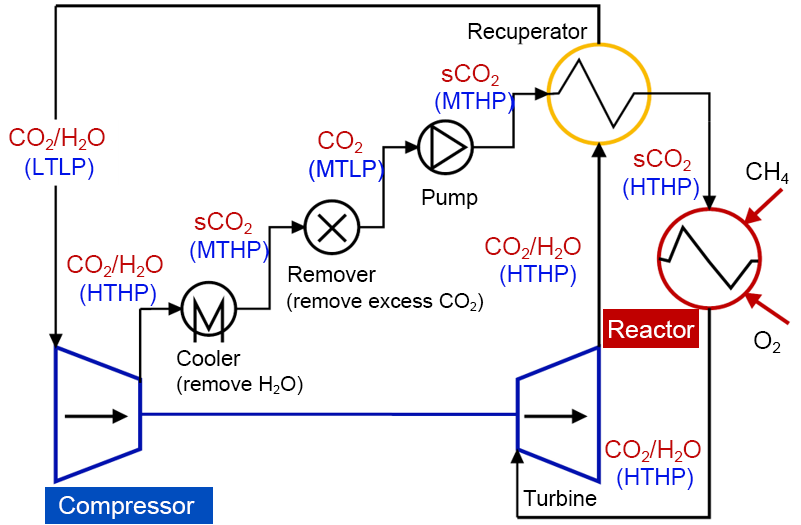
\includegraphics[width=0.6\linewidth]{schematic_cycle.png}
        \end{center}
        \caption{Schematic of a \ce{sCO2} gas turbine cycle with oxy-combustion thermal input.}
        \label{fig1}
    \end{figure}

    %\subsection{Traditional closed \ce{sCO2} cycle vs. semi-closed \ce{sCO2} gas turbine cycle}\label{app:sCO2cycle:TwoCycleComp}
    %The advantages of traditional closed \ce{sCO2} cycle with a single working fluid and an external heater have been summarized in the literature \citep{ahn2015review}:

    %\noindent$\bullet$ \textbf{Higher efficiency}: \ce{sCO2} is considered to remain in a single-phase throughout the entire cycle. Hence, there is no requirement for additional energy to evaporate liquid phase to gas phase or condense gas to liquid phase like the traditional steam Rankine cycle, leading to a greater energy conversion efficiency.

    %\noindent$\bullet$ \textbf{Higher efficiency}: \ce{sCO2} cycle combines the advantages of both steam Rankine cycle and gas turbine Brayton cycle to achieve higher thermal efficiency. In other words, the fluid is compressed in the low compressibility region (either  the subcritical liquid region or supercritical liquid-like region, to reduce the associated compression work~\cite{ahn2015review}), and high turbine inlet temperature is utilized.

    %\noindent$\bullet$ \textbf{Smaller turbomachinery size}: as the system operates beyond the critical point, $P_{c, CO_2}$ ($\sim$7.4 MPa), \ce{sCO2} remains dense with high enthalpy throughout the entire cycle. For this reason, the fluid volume and volumetric flow rate can be reduced significantly to maintain the same energy supply, resulting in compact turbomachinery compared to that of a steam cycle.

    %\noindent$\bullet$ \textbf{Smaller turbomachinery size}: As the system operates beyond the critical pressure of \ce{CO2}, $P_{c, CO_2}$ ($\sim$7.4 MPa), the minimum pressure of \ce{sCO2} cycle is higher than any existing steam Rankine cycle (a few kPa) or gas turbine Brayton cycle ($\sim$100 kPa), and hence the reduced pressure is generally larger than 1 and lower than 3, but the reduced temperature in the system is still near 1. Thus the pressure is relatively high but temperature is relatively low, and \ce{CO2} remains dense with high enthalpy throughout the entire cycle. For this reason, the fluid volume and volumetric flow rate can be reduced significantly to maintain the same energy supply, resulting in a very compact turbomachinery compared to that of a steam cycle.

    %However, these advantages are for the traditional closed \ce{sCO2} cycle with an external heater, which use nuclear or coal combustion as the energy source to heat the single working fluid of \ce{sCO2}. Therefore, whether these advantages are still evident for the semi-closed \ce{sCO2} gas turbine cycle needs to be evaluated. Although the oxy-combustion under \ce{sCO2} conditions are more convenient, environmentally friendly, and sustainable, it lacks investigation.

    %\subsection{\ce{sCO2} compressor}\label{app:sCO2cycle:compressor}
    %Baltadjiev et al. \cite{baltadjiev2015investigation} analyzed a \ce{sCO2} compressor at various operating conditions and suggested that nucleation is likely to occur at the leading edge of the impeller as the critical point is approached due to the local flow acceleration. Brinckman et al. \cite{brinckman2019numerical} used a non-equilibrium phase-change model and found that there is sufficient residence time in the compressor to form the droplets. 
    %These works only consider the pure \ce{CO2} as the working fluid. 
    %The cooler in the semi-closed \ce{sCO2} gas turbine cycle (see Fig.~\ref{fig1}) cannot remove all of the \ce{H2O}, so there will be a small amount of \ce{H2O} in the whole system. For this reason, the compressor was carried out with a mixture of \ce{CO2}/\ce{H2O} as the working fluid instead of pure \ce{CO2} in the traditional closed \ce{sCO2} cycle. Since \ce{H2O} has a very high critical pressure, the thermodynamic properties of the working fluid change a lot, especially the real mixture critical point which depends on the composition of the mixture and could be far away from that of pure \ce{CO2}. Hence, although the operating pressure are in the supercritical region of pure \ce{CO2}, they could still be lower than mixture critical pressure, which means that the working fluid mixture could be in a subcritical two-phase state rather than a supercritical single-phase state, and the liquid droplets formed in the compressor could cause erosion.
    %On the other hand, the supercritical fluid, such as \ce{sCO2}, holds high energy density $\rho e$ near its critical point due to the large variation of density $\rho$, which results in a large change in specific heat capacity $c_p$ for a small temperature change. Therefore, it is better to keep the fluid temperature close to the critical point to take this special advantage of high energy density to compact the turbomachinery.
    %Both subcritical liquid fluid and supercritical liquid-like fluid have low compressibility to reduce the compression work necessary for a given pressure ratio \citep{ahn2015review,invernizzi2017prospects}, which is a motivation to keep the working fluid close to its critical point so that the compressor can work under these conditions. Accordingly, an accurate determination of the mixture critical point becomes very important. 
    %In \ref{thermo analysis}, the evolution of mixture critical point and the compressibility in the compressor is evaluated.
    %In \label{thermo analysis} one of the main tasks is to evaluate the evolution of mixture critical point and the thermal/transport properties in the compressor (see Sec.~\ref{sec:result:compressor}), which are expected to control the thermal efficiency of the overall system and assist the design of recuperator, compressors, and the following cooler, remover, as well as the pump (see Fig.~\ref{fig1}).
    %In this study, one of the main tasks is to evaluate the evolution of mixture critical point and the thermal/transport properties in the compressor (see Sec.~\ref{sec:result:compressor}), which are expected to control the thermal efficiency of the overall system and assist the design of recuperator, compressors, and the following cooler, remover, as well as the pump (see Fig.~\ref{fig1} in \ref{app:sCO2cycle}).

    %\subsection{\ce{sCO2} oxy-combustor}\label{app:sCO2cycle:combustor}
    %In \ce{sCO2} oxy-combustor (i.e., the reactor in Fig.~\ref{fig1}), %although the high temperature of combustion prevents the liquid phase from forming, in the cold ignition process, the 
    %phase separation may still occur due to the mixing between working fluid (\ce{CO2}/\ce{H2O}) and injected \ce{O2} and \ce{CH4}.
    %In the reactor (i.e., the oxy-combustor), the working fluid is composed of \ce{CO2}, \ce{H2O}, \ce{CH4}, and \ce{O2}. The real mixture critical point is also different from that of a single fluid.
    %For the pure gas phase, the mass mixing time scale is tiny due to the large mass diffusivity, and the corresponding ``effective'' ignition delay is also shortened. However, if the mixture is in a two-phase state (and hence droplets will be formed), the mass diffusivity is decreased, and the mass mixing time is increased. In contrast, the thermal diffusivity is increased for two-phase fluid, and the thermal conduction time is reduced. Therefore, the droplets formed in mixing processes may affect the cold ignition in terms of ``effective'' ignition delay. In addition, phase separation might lead to combustion-induced Rapid Phase Transition (cRPT)~\citep{basco2013effect}, which causes anomalous high or oscillating pressures to damage the equipment and cause safety issues. %In this work, the model is still not able to analyse the combustion process, we focus on the mixing and phase split.

    %As part of the effort to understand the ``effective'' ignition delays for the mixtures of \ce{CH4}/\ce{O2}/\ce{CO2} with excess \ce{CO2}, knowledge of the thermodynamic phase state and properties at the target oxy-combustor operating conditions is required.
    %In addition, the temperature of injected \ce{CH4} and \ce{O2} are lower than the ambient temperature, which might be cold enough to condense \ce{H2O} in the mixture. Hence, phase separation might occur near the injector of fuel or oxidizer, and the mixture could partially be condensed into small droplets.

    %In addition, close to the real mixture critical point (C.P.), the heat and mass transfer is very different from that away from the critical point. Small temperature changes lead to large changes in the transport properties \citep{sengers1985transport}, and significant heat/mass transfer enhancement or deterioration can occur. The \ce{sCO2} fluid holds high energy density near its critical point, and the significant variation of \ce{sCO2} thermophysical properties in the near-critical-point region differentiates the heat transfer and flow mechanism from conventional fluids. Particularly, the abrupt increase of specific heat greatly increases the heat-transfer coefficient which reaches its peak at the critical point. Therefore, it is better to keep the fluid conditions close to the critical point to take this special advantage, and the determination of the mixture critical point becomes very important.
\comment{
    \section{VLE solvers: TPn flash solver and HPn flash solver} \label{app:VLE}
    \textbf{Isothermal and isobaric (TPn) flash solver:}
    VLE is governed by fugacity equality Eq.~(\ref{eq:4}) and Rachford-Rice equation \citep{rachford1952procedure} Eq.~(\ref{eq:5}), which is an additional constraint to the equilibrium solver as used in Ref.~\citep{saha1997isoenergetic} and obtained from the conservation of each component.
    \begin{equation}
        f_{i, l}\big/f_{i, g}=1\label{eq:4}
    \end{equation}
    \begin{equation}
        \sum_{i=1}^{N}\bigg\{z_i\left(1-K_i\right)\bigg/\left[1+\left(K_i-1\right)\psi_{g}\right]\bigg\}=0\label{eq:5}
    \end{equation}
    \begin{equation}
        K_i=y_i/x_i \label{eq:5-1}
    \end{equation}
    \begin{equation}
        \sum_{i=1}^{N}x_i=\sum_{i=1}^{N}y_i=1\label{eq:5-2}
    \end{equation}
    where $f_{i, p}$ is the fugacity of component $i$ in phase $p$ ($p=l$: liquid; $p=g$: gas), $x_i$ is the mole fraction of component $i$ in liquid phase, $y_i$ is the mole fraction of component $i$ in gas phase, $z_i$ is the overall mole fraction of component $i$, $\psi_g$ is the gas mole fraction, and $K_i$ is the equilibrium constant of component $i$. %Eq.~(\ref{eq:5}) is the Rachford-Rice equation, which is an additional constraint to the equilibrium solver as used in \citet{saha1997isoenergetic} obtained from the conservation of each component.

    The real-fluid properties are described using the Peng-Robinson equation of state (PR-EOS) \citep{peng1976new}:
    \begin{equation}
        P=\frac{RT}{V_p-b_p}-\frac{a_{p}}{V_p\left(V_{p}+b_p\right)+b_p\left(V_p-b_p\right)} %\nonumber \\&\left(p=1\rm{: gas};\quad p=2\rm{: liquid}\right)
        \label{eq:preos}
    \end{equation}
    where $P$, $R$, and $T$ are pressure, gas constant, and temperature, respectively, which are the known variables. $V_p$ is the specific volume of phase $p$, which is the unknown to be solved from PR-EOS. The $a_p$ and $b_p$ are PR-EOS coefficients of each phase, which are calculated from the corresponding single component coefficients $a_i$ and $b_i$ using the mixing rule described in Ref.~\citep{reid1977properties}:
    \begin{align}
        a_g= & \sum_i\sum_jy_iy_j(1-b_{ij})\sqrt{a_ia_j} \label{eq:ap} \\
        a_l= & \sum_i\sum_jx_ix_j(1-b_{ij})\sqrt{a_ia_j}               \\
        b_g= & \sum_iy_i b_i                                           \\
        b_l= & \sum_ix_i b_i \label{eq:bp}
    \end{align}
    where %$x_i$ is the mole fraction of component $i$ in liquid phase (subscript $l$), and $y_i$ is the mole fraction of component $i$ in gas phase (subscript $g$). 
    $b_{ij}$ is a binary interaction parameter. For every component $i$, the single component coefficients $a_i$ and $b_i$ are given by
    \begin{align}
        a_i= & 0.45724\frac{R^2 T_c^2}{P_c} \hat{a}_i \label{eq:ai} \\
        b_i= & 0.07780\frac{RT_c}{P_c} \label{eq:bi}
    \end{align}
    where subscript ``$c$'' means critical value, and $\hat{a}_i$ is given by
    \begin{equation}
        \hat{a}_i=(1+\kappa(1-T_r^{1/2}))^2
    \end{equation}
    where subscript ``$r$" means the reduced value (e.g., $T_r=T/T_c$).
    \begin{equation}
        \kappa=0.37464+1.54226\omega-0.26992\omega^2 \label{eq:kappa}
    \end{equation}
    where $\omega$ is the acentric factor. 
    The fugacity formula of PR-EOS is shown below \citep{yi2019multicomponent}:

    \begin{align}
         & f_{i,g}=P y_i \exp \left[\frac{B_i(Z - 1)}{B_{mix}} - ln(Z-B_{mix})- \frac{A_{mix}} {2\sqrt{2} B_{mix}} \right. \nonumber\label{fuga}                                                \\
         & \left.\times\left(\frac{2 \sum_j {x_j A_j} } {A_{mix}} - \frac {B_i} {B_{mix}}\right) ln\left(\frac{Z + (1+\sqrt{2})B_{mix}} { Z + (1-\sqrt{2}) B_{mix}}\right)\right]                \\
         & f_{i,l}=P x_i \exp \left[\frac{B_i(Z - 1)}{B_{mix}} - ln(Z-B_{mix})- \frac{A_{mix}} {2\sqrt{2} B_{mix}}  \right. \nonumber                                                            \\
         & \left.\times \left(\frac{2 \sum_j {x_j A_j} } {A_{mix}} - \frac {B_i} {B_{mix}}\right) ln\left(\frac{Z + (1+\sqrt{2})B_{mix}} { Z + (1-\sqrt{2}) B_{mix}}\right)\right]  
    \end{align}

    where
    \begin{align}
         & A_i=\frac{a_i P}{R^2T^2} \label{fuga 1}                           \\
         & B_i=\frac{b_i P}{RT}                                              \\
         & A_{mix}=\sum_i\sum_jx_ix_j(1-b_{ij})\sqrt{A_iA_j}                 \\
         & B_{mix}=\sum_ix_i B_i                                             \\
         & Z=\frac{PV}{RT}\text{ (compressibility factor)}  \label{fuga end}
    \end{align}

    The equation set of Eqs.~(\ref{eq:4}-\ref{eq:kappa}, \ref{fuga}-\ref{fuga end}) is solved based on Newton's method. The flow chart of TPn flash solver is shown in Fig.~\ref{FC}. The initial guess is obtained using Wilson Equation \citep{wilson1964vapor}:
    \begin{equation}
        K_i=e^{5.373(1+\omega_i)(1-1/T_{r,i})}/P_{r,i}
    \end{equation}
    where $\omega_i$ is the acentric factor of component $i$; $T_{r,i}$ and $P_{r,i}$ are the reduced temperature and reduced pressure of component $i$, respectively.
    Then, solving the Rachford-Rice equation (i.e., Eq.~(\ref{eq:5})) using Newton's method to get $\psi_g$. $x_i$ and $y_i$ can be obtained from Eqs. (\ref{eq:5-1}) and (\ref{eq:5-2}). The next step is to evaluate fugacity using the Eqs. (\ref{fuga}-\ref{fuga end}), and examine whether fugacity equilibrium (i.e., $f_{i,l}=f_{i,g}$) has been reached. If not, update $K_i$ by $K_i=K_i \times f_{i,l}/f_{i,g}$ and go back to solve the Rachford-Rice equation (i.e., Eq.~(\ref{eq:5})). When the error is less than a tolerance (i.e., the Newton iteration is converged), the solver will break the loop and output the solution.

    As discussed above, each phase always follows its own PR-EOS, and the constrain of phase equilibrium (Eqs.~(\ref{eq:4}-\ref{eq:5-2})) connects the two phases. This is the so-called ``composite EOS'' method, which can avoid the negative squared speed of sound and was used in Ping et al.'s work \cite{yi2019multicomponent}.
    \begin{figure}[htbp]
        \centering
        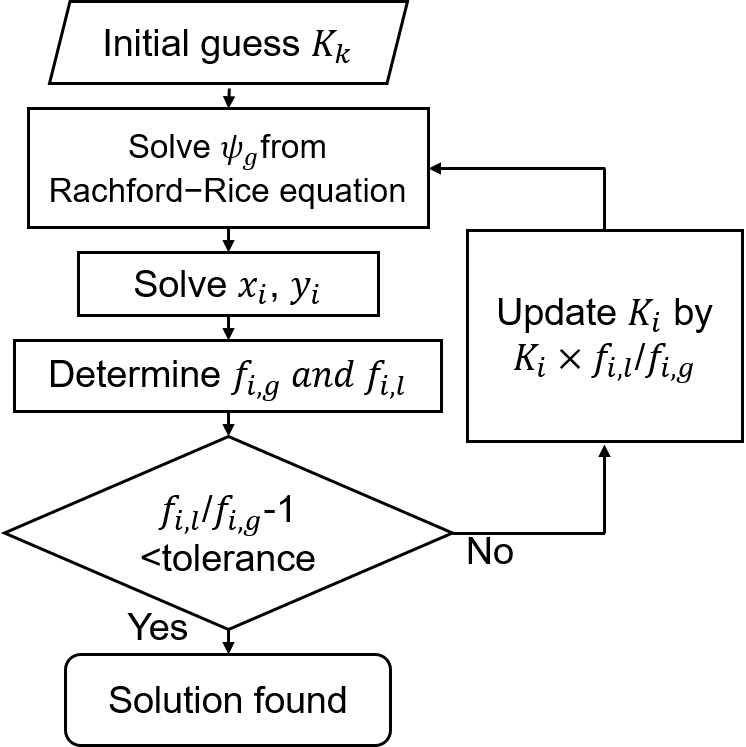
\includegraphics[width=0.5\linewidth]{flow_TPn_v2.png}
        \caption{Flow chart of the TPn flash solver.}
        \label{FC}
    \end{figure}
    Mixture enthalpy and density are evaluate using the solution obtained from the TPn flash.  
    \begin{flalign}
        \begin{cases} 
            Z =\psi_g Z_g + (1-\psi_g)Z_l                  \\
            \rho=\frac{pM}{ZRT} \\
            h=\sum y_{p}h_{p}
        \end{cases}\label{eq:3}
    \end{flalign}
    where $y_p$, and $h_p$ are the phase mass fraction ($y_g=\psi_g\frac{M_g}{M} $ in Eq.~(\ref{eq:5})), and phase specific internal enthalpy, respectively, with $p=1$ for gas (index $g$) and $p=2$ for liquid (index $l$).
    \textbf{Isobaric and Isenthalpic (HPn) flash solver:}
    %In adiabatic mixing processes, the mixture properties are often assumed as simple functions of temperature at specified pressure and overall compositions. However, as pointed out by Qiu et al. \citep{qiu2014development}, this assumption is not good because the thermal solution must ensure the Gibbs energy of the mixture to be at global minimum. It means that the enthalpy is not only a function of temperature but also a function of the number of phases and their properties. 
    The equilibrium temperature $T_{eq}$ at specified pressure (P), enthalpy (H), and overall compositions (n) is calculated by the HPn flash solver and the corresponding objective function is expressed as
    \begin{equation}
        F_{h}=\left(h^{*}-h_{eq}\right)/h^{*}\label{eq:6}
    \end{equation}
    where $h^{*}$ is the specific mixture enthalpy, which is calculated based on the linear mixing rule as
    \begin{equation}
        h^{*}=\sum_{i=1}^{N}z_i h_i\left(T_i, P\right)\label{eq:7}
    \end{equation}
    where $T_i$ is the temperature of component $i$ before the mixing. The partial enthalpy $h_i$ of component $i$ is calculated as
    \begin{equation}
        h_i\left(T_i, P\right)=h_{i, ideal}\left(T_i, P\right)+h_{i, dep}\left(T_i, P\right)
    \end{equation}
    where $h_{i, ideal}$ is the enthalpy of component $i$ in ideal gas state, which is evaluated by JANAF polynomials; and $h_{dep}$ is the departure enthalpy, which is derived based on the PR-EOS, calculated as
    \begin{equation}
        h_{i, dep}\left(T_i, P\right)=RT_i\left(Z_i-1\right)+\frac{T_i da_i/dT_i-a_i}{2\sqrt{2}b_i}ln\frac{Z_i+\left(1+\sqrt{2}\right)B_i}{Z_i+\left(1-\sqrt{2}\right)B_i}\label{eq:8}
    \end{equation}
    %Both $h_{i, ideal}$ and $h_{dep}$ have the unit of J/mol. 
    $h_{eq}$ is the equilibrium enthalpy calculated as
    \begin{equation}
        h_{eq}=\psi_{g}h_{g}+\left(1-\psi_{g}\right)h_{l}\label{eq:9}
    \end{equation}
    where $\psi_g$ is the gas mole fraction, which is obtained from the TPn flash solver. The phase enthalpy $h_g$ and $h_l$ are calculated using the similar formulas as
    \begin{align}
         & h_{p}=h_{p, ideal}+h_{p, dep}                                                                                                                                                       \\
         & h_{p, dep}=RT_{eq}\left(Z_{p}-1\right)+\frac{T_{eq} da_{p}/dT_{eq}-a_{p}}{2\sqrt{2}b_p}ln\frac{Z_{p}+\left(1+\sqrt{2}\right)B_{p}}{Z_{p}+\left(1-\sqrt{2}\right)B_{p}}\label{eq:10}
    \end{align}
    \begin{equation}
        h_{l, ideal}=\sum_ix_ih_{i, l, ideal},\quad h_{g, ideal}=\sum_iy_ih_{i, g, ideal}\label{eq:11}
    \end{equation}
    Equilibrium temperature $T_{eq}$ is updated in the HPn flash solver iteratively as
    \begin{equation}
        T_{n}=T_{n-1}+\left(h^{*}-h_{eq, n-1}\right)\Big/C_{p,n-1}\label{eq:12}
    \end{equation}
    where $C_{p,n-1}=(h_{eq, n-1}-h_{eq, n-2})/(T_{n-1}-T_{n-2})$ and $n$ is the iteration index.
    %\begin{equation}
    %    T_{n}=T_{n-1}+\left(h^{*}-h_{eq, n}\right)\Big/C_{p, mix, n}\label{eq:12}
    %\end{equation}
    %where $C_{P, mix, n}$ is calculated at time-step $n$ (for conciseness, subscript $n$ is neglected in the following) as
    %\begin{equation}
    %    C_{P, mix}=\sum C_{P, p}\alpha_{p}\label{eq:13} 
    %\end{equation}
    %\begin{equation}
    %    C_{P, p}=C_{V, p}-\frac{T}{\rho_{p}}\left(\left.\frac{\partial p}{\partial T}\right|_{\rho_{p}}\right)^{2}\Bigg/\left.\frac{\partial p}{\partial\rho_{p}}\right|_{T}\label{eq:14}
    %\end{equation}
    %\begin{equation}
    %    C_{V, p}=\text{\ensuremath{\frac{e_{p}\left(T+\Delta T, V_p\right)-e_{p}\left(T, V_p\right)}{\Delta T}}}\label{eq:15}
    %\end{equation}
    %\begin{equation}
    %    \left.\frac{\partial p}{\partial T}\right|_{\rho_p}=\frac{R}{V_p-b_p}-\frac{\partial\alpha_{p}}{\partial T}\frac{1}{V_p^{2}+2b_pV_p-b_p^{2}}\label{eq:16}
    %\end{equation}
    %\begin{equation}
    %    \left.\frac{\partial p}{\partial\rho_{p}}\right|_T=-\frac{MW_{p}}{\rho_{p}^{2}}\left[\frac{-RT}{\left(V_p-b_p\right)^{2}}+\frac{2a_{p}\left(b_p+V_p\right)}{\left(V_p^{2}+2b_pV_p-b_p^{2}\right)^{2}}\right]\label{eq:17}
    %\end{equation}
    %\begin{equation}
    %    \rho_{p}=MW_{p}/V_p, \alpha_{p}=V_p\bigg/\sum V_p\label{eq:18}
    %\end{equation}
    %where $\alpha_p$, $\rho_p$, and $MW_p$ are phase volume fraction, density, and molecular weight, respectively. $V_p$ is the phase specific volume calculated from the PR-EOS Eq.~(\ref{eq:preos}) based on the phase compositions, and $a_p$ and $b_p$ are the PR-EOS coefficients calculated using Eqs.~(\ref{eq:ap}-\ref{eq:bp}) based on the phase compositions. 

    During the calculation, the system is always considered as a two-phase system, in which the phase composition indicates the mole fraction of each species in each phase. When $\psi_g \leq10^{-4}$, the fluid is considered as a pure liquid; when $\psi_g \geq 1-10^{-4}$, the fluid is considered as a pure gas. %  For pure liquid phase state, a virtual amount of gas phase is added, which is set as $\alpha_{\rm{virtual}}=10^{-4}$ in this study, and vice versa for pure gas phase state. In the isobaric and isenthalpic (HPn) mixing process, Newton's iterative method is used to obtain the equilibrium temperature $T_{eq}$ at given pressure and enthalpy, and then the phase compositions are calculated at the specific pressure $P$ and equilibrium temperature $T_{eq}$.
    In CFD simulation, the thermodynamic properties are updated using the HPn flash results at each time step, as shown in Fig.~\ref{FC_CFD}.
    
    Note that although the VLE model does not consider non-equilibrium effect of phase change, Mo and Qiao's molecular dynamics (MD) simulation results \cite{mo2017molecular} showed that when subcritical flow enters the supercritical regime, it only needs about 1 ns for surface tension to vanish, which indicates that phase equilibrium is reached ``immediately'' with respect to a typical time step size, and the phase change is dominated by slower diffusion processes. Hence the VLE model should be able to capture the phase change effects accurately.
    

}
    %\textbf{Another important application of VLE solvers:}
    %Both Roy and Segal's experimental results \citep{roy2010experimental} and Banuti and Hannemann's simulation work \citep{banuti2016absence} show different break-up behaviors under supercritical conditions, which may be dominated by thermal disintegration rather than classical mechanical break-up. The determination of fluid state is very important to understand which disintegration mechanism controls liquid propellant atomization. Therefore, in addition to \ce{sCO2} gas turbine systems, another important application of VLE solvers is high-pressure liquid propellants injection (e.g., in diesel engines, aircraft jet engines, and liquid rocket engines).
\comment{
    \section{Pressure Poisson equation in the PIMPLE algorithm} \label{App:gp}
    
    In PIMPLE, the momentum equations (Eq.~(\ref{Gm})) are linearly discretized into the following matrix form:
    \begin{equation}
        A u+ \sum_{ne} A_{ne} u_{ne} =S+\nabla P \label{p0}
    \end{equation}
    where $u_{ne}$ is the velocity of a neighbor gird point $ne$, $A$ and $A_{ne}$ are the matrix coefficients corresponding to the current and neighbor grid points, respectively, and all other terms are denoted as $S$. Rearranging Eq.~(\ref{p0}) gives the following form:
    \begin{align}
         & u=H^*-\frac{\nabla P}{A}\label{p1}       \\
         & H^* =\frac{S-\sum_{ne} A_{ne} u_{ne}}{A}
    \end{align}
    Substituting EOS (i.e., Eq.~(\ref{EOS})) and Eq.~(\ref{p1}) into the continuity equation (Eq.~(\ref{G:start})) gives the pressure Poisson equation:
    \begin{align}
        \text{Subsonic: }  & \frac{\partial\phi P}{\partial t}+\nabla\cdot \Bigg[\rho \bigg(H^*- \frac{\nabla P}{A}\bigg)\Bigg]=0 \label{p2}         \\
        \text{Transonic: } & \frac{\partial\phi P}{\partial t}+\nabla\cdot (\phi P H^*)-\nabla\cdot \bigg(\rho \frac{\nabla P}{A}\bigg)=0 \label{p3}
        % &\frac{\rho_{*}-\rho_n}{\Delta t}+\frac{\partial \rho_n u_i^n}{\partial x_i}=0\\
        % &\frac{\rho^{*}u^{*}_i-\rho_n u_i^n}{\Delta t}+\frac{\partial \rho_n u_j^nu^{*}_i}{\partial x_j}=-\frac{\partial P_n}{\partial x_i}+\frac{\partial \tau_{ij}}{\partial x_j}\\
        % &\frac{\rho^{*}Y^{*}_m-\rho_n Y_m^n}{\Delta t}+\frac{\partial \rho^{*} u_j^{*}Y_m^{*}}{\partial x_i}=\frac{\partial }{\partial x_j}\left(\rho D \sum_m h_m \frac{\partial Y_m^{*}}{\partial x_j}\right)\\
        % &\frac{\rho^{*}h_{*}-\rho_n h_n}{\Delta t}+\frac{\partial \rho_n u_j^{*}h_{*}}{\partial x_j}+\frac{\partial \rho K}{\partial t}+\frac{\partial \rho_n u_j^{*}K}{\partial x_j}-\frac{\partial P_n}{\partial t}=-\frac{\partial q_i}{\partial x_i} +\frac{\partial \tau_{ij}u_j^{*}}{\partial x_i}\\
    \end{align}
    Eq.~(\ref{p2}) and Eq.~(\ref{p3}) are used for pressure update. Eq.~(\ref{p3}) is obtained by substituting EOS (i.e., Eq.~(\ref{EOS})) into the second term of Eq.~(\ref{p2}). With this change, the solver is able to capture the compressibility better. Hence, Eqs.~(\ref{p2}) and (\ref{p3}) are used to solve subsonic and transonic flows, respectively.
    }
    
    \section{VLE-based tabulation method} \label{App:tab} % and its verification
    
    A tabulation method is used to accelerate VLE model computation. This method is used to replace the computationally expensive on-the-fly TPn flash. Within the given range of temperature, pressure, and mass fraction, TPn problems are solved on the evenly spaced grid points. Then the thermodynamic proprieties (including $\rho$, $h$, $c_v$, $c_p$) and  transport  proprieties (including $D_m$, $\mu$, $\alpha$) are evaluated using TPn solutions. 
    The TPn solutions and all properties are recorded into the table. When retrieving the solution of given input ($T^*$, $p^*$, $x^*$), linear interpolation is used:
    \begin{enumerate}
     \item Find the closest temperature, pressure and mass fraction in the table, 
     $T_1 \leq T^* < T_2 $,
     $p_1 \leq p^* < p_2 $,
     $x_1 \leq x^* < x_2 $
     \item Calculate the weight for linear interpolation,
     $ \alpha^v_1=\frac{v_2-v^*}{v_2-v_1}$,
     $ \alpha^v_2=\frac{v^*-v_1}{v_2-v_1}$, $v=T,p,x$
     \item For any property $A$ in the table, linear interpolation uses the formula $A^* = \sum_{i,j,k=1,2}\alpha^T_i \alpha^p_i \alpha^x_i A_{ijk} $
    \end{enumerate}
    
    To mitigate the concern about potential VLE-inconsistency, an accuracy test is provided here. The same shock tube case as the one in Sec.~\ref{sec:results:ShockTube} is used to test the tabulation method. The shock tube condition is shown in Table~\ref{conditions}.
    The table used for the simulation covers the temperature range of 470-600 K, pressure range of 9-25 MPa, and $x_{\ce{CO2}}$ range of 0.6-0.9. The table grid sizes are $\Delta T = 1.3$ K, $\Delta p = 0.4$ MPa, and $\Delta x_{\ce{CO2}} = 0.015$.
    The $L^{\infty}$ absolute error (i.e., $max(\Delta A)$), maximum local relative error (i.e., $max(\frac{\Delta A}{A})$), and $L^2$ relative error (i.e., $ \frac{\|\Delta A\|_{L^2}}{\|A\|_{L^2}}$) are obtained by comparing to the results without tabulation, and shown in Table.~\ref{table:error}. The results show that the maximum local errors are controlled within 10\% and the $L^2$ errors are control within 5\%.

    \begin{table}[htbp]
        %\begin{center}
        \centering
        \begin{minipage}{0.9\textwidth}
            \caption{Relative error of VLE-based tabulation method.} \label{table:error}
            \begin{center}
                \begin{tabular}{@{}l|lll@{}} %\hline
                    \toprule
                                    &Pressure  & Density   & Gas Mole Frac.   \\ %\hline
                    \midrule
                    $L^{\infty}$ absolute error           & 0.17 MPa        & 5.889 $kg/m^3$   & 0.02\\%\hline
                    maximum local relative error          &  1.4\%           & 1.6\%   & 2.1\% \\ %\hline
                     $L^2$ relative error               &  0.09\%           & 0.09\%   & 0.1\% \\ %\hline
                    \bottomrule
                \end{tabular}

            \end{center}
        \end{minipage}
        %\end{center}

    \end{table}

    \section{Validation and verification of the VLE solvers and CFD solver} \label{App:vali}


    \subsection{Validation of the TPn flash solver based on phase boundaries}
    The TPn flash solver is validated by comparing the predictions with the experimental data of Somait and Kidnay~\cite{somait1978liquid} in terms of the phase boundaries of \ce{CO2}/\ce{CH4} and \ce{CO2}/\ce{H2O} mixtures. As shown in Fig.~\ref{v1}, the model prediction agrees with the experimental data very well for both mixtures.
    \begin{figure}[htbp]
        \centering
        \subfigure{
            %\begin{minipage}[t]{0.5\linewidth}
            \centering
            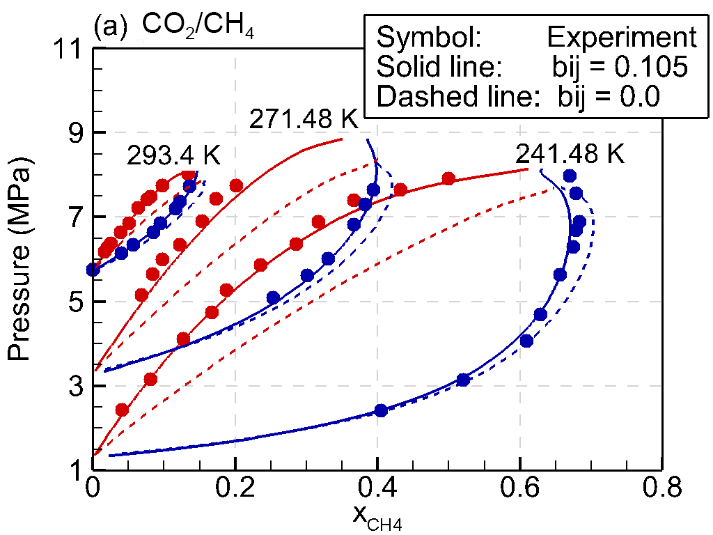
\includegraphics[width=0.45\linewidth]{phase_diagram_PX_CO2_CH4.png}
            %\caption{fig1}
            %\end{minipage}%
        }%
        \subfigure{
            %\begin{minipage}[t]{0.5\linewidth}
            \centering
            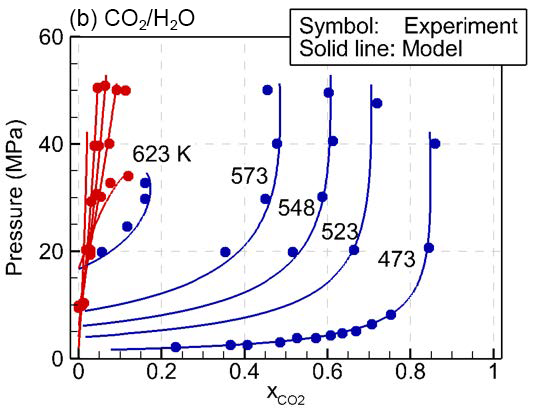
\includegraphics[width=0.45\linewidth]{phase_diagram_PX_CO2_H2O.png}
            %\caption{fig2}
            %\end{minipage}%
        }%
        \caption{Comparison of pressure-composition phase boundaries between experimental measurements and model predictions: (a) mixtures of \ce{CO2} and \ce{CH4}; (b) mixtures of \ce{CO2} and \ce{H2O}. Symbol: experimental data \citep{somait1978liquid}; line: model prediction. In sub-figure (a), solid line: binary interaction parameter $b_{ij}=0.105$ is used in Eqs.~(6-7) of the Supplementary Material; dashed line: $b_{ij}=0$ is used in Eqs.~(6-7) of the Supplementary Material. Red color: bubble points/curve, blue color: dew points/curve.}
        \label{v1}
    \end{figure}

    \subsection{Verification of the TPn flash solver based on mixture critical points}
    Next, the mixture critical points obtained from the VLE method (specifically, the TPn flash solver) are compared with those obtained from several other methods. In the VLE-based method, critical points can be obtained directly from the intersection of the dew curve and bubble curve.

    Stradi et al.~\cite{stradi2001reliable} derived the mixture critical point based on Heidemann and Khalil's criticality formulation~\cite{heidemann1980calculation} as below, which has been widely used due to its clear theoretical foundation. For a mixture of $C$ components,
    \begin{align}
         & Q\Delta \mathbf n=\mathbf0                                                                          \\
         & Q_{ij}=\left( \frac{\partial^2A}{\partial n_i \partial n_j}\right)_{T,V}                            \\
         & \sum_i^{C}\sum_{j}^{C}\sum_{k}^{C}A_{ijk}\Delta n_i\Delta n_{j}\Delta n_{k}=0                       \\
         & \Delta \mathbf n^{T}\Delta \mathbf n=1                                                              \\
         & A_{ijk}=\left( \frac{\partial^3A}{\partial n_i \partial n_j\partial n_k}\right)_{T,V} \label{eq:19}
    \end{align}
    where $\Delta \mathbf n$ means the nonzero perturbation vector of the component mole numbers; $A$ is the Helmholtz free energy. Since the Helmholtz free energy depends on the mixture composition, this way is implicitly dependent on the local mixture. The binary critical points predicted by the above methods are compared in Fig.~\ref{v2}, and the predictions of the current VLE-based method agree very well with Stradi et al.'s formulation~\cite{stradi2001reliable} for the mixture of \ce{CH4} and \ce{H2S}. But note that Stradi et al.'s formulation can only predict critical points, and it cannot provide other detailed information (e.g., phase boundaries) about phase diagrams like what VLE solver can provide.


    \begin{figure}[htbp]
        \begin{center}
            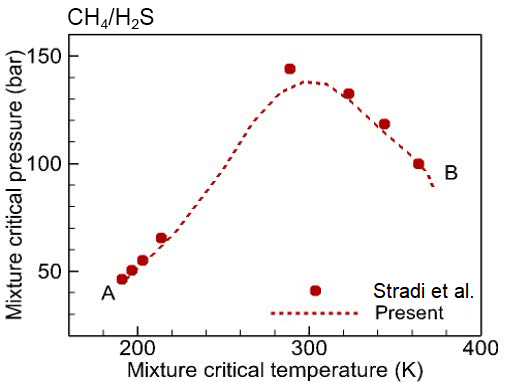
\includegraphics[width=0.55\linewidth]{critical_point_CH4_H2S.png}
            %\includegraphics[width=0.45\linewidth]{thermal/vali2_v2.png}
        \end{center}
        \caption{Comparison of predicted mixture critical points of \ce{CH4}/\ce{H2S} mixtures between Stradi et al.~\cite{stradi2001reliable} and the present work (overall mole fraction of \ce{CH4} is increased from 0.01 at A to 0.99 at B).
        }
        \label{v2}
    \end{figure}

    \subsection{Verification of HPn flash solver based on equilibrium mixing temperature $T_{eq}$}
    All the validation and verification above are for the TPn flash solver. Here, the HPn flash solver is verified by the Fig. 1(b) in Matheis and Hickel~\cite{matheis2018multi}. As shown in Fig.~\ref{v6}, the present prediction of equilibrium mixing temperature $T_{eq}$ agrees with Matheis and Hickel's result very well.
    \begin{figure}[htb]
        \begin{center}
            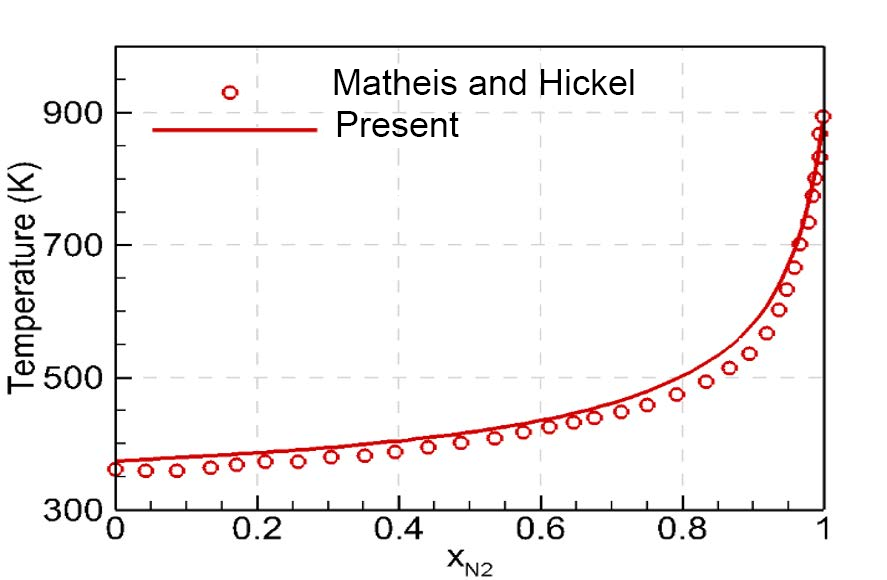
\includegraphics[width=0.50\linewidth]{mixing_temperature_C12_N2.png}
        \end{center}
        \caption{Comparison of predicted equilibrium mixing temperatures $T_{eq}$ for n-dodecane/nitrogen mixtures between Matheis and Hickel~\cite{matheis2018multi} and the current model.}
        \label{v6}
    \end{figure}

    \subsection{Validation and verification of the CFD solver} \label{App:vali:CFD}
    Two 1D shock tube simulations are conducted to validate and verify the CFD solver. First, Sod shock tube~\cite{sod1978survey} is used to test the CFD solver with the ideal gas model, and the results are shown in Fig.~\ref{vali1ST}. The pressure and temperature evolution show a good agreement with the exact solution. Although the PIMPLE algorithm is pressure-based, the 1D Sod shock tube results clearly show that this compressible version of PIMPLE algorithm can well capture the shock wave and accurately predict compressible flows. Moreover, the results show that the scheme is not dissipative, as the sharp gradients (e.g., near the shock) are accurately captured with only 200 grid cells and there is no spurious oscillation near the high gradients. Second, results from a shock tube simulation with phase change are compared with Chiapolino et al.'s simulation results~\cite{chiapolino2017simple}, as shown in Fig.~\ref{vali2ST}. The shock tube is filled with a homogeneous water-air mixture, and the initial discontinuity is located at 0.5 m. Chiapolino et al.'s model used the Noble Abel Stiffened Gas (NASG) EOS and also assumed mechanical and thermodynamic equilibrium. Therefore, their results can also capture the phase change in the shock tube, which is valuable as a reference to verify the implementation of the VLE-based CFD simulation framework in this study both qualitatively and quantitatively. Good agreements were obtained in terms of the evolution of pressure and temperature at the contact discontinuity.
    Note that Chiapolino et al. used a fully compressible CFD solver (based on MUSCL Hancock method using van Leer’s slope limiter and HLLC Riemann solver), while the CFD solver in this study uses a pressure-based PIMPLE method (which can be called a ``low-Mach'' solver but was extended to a transonic version). For this reason, the fact that both CFD solvers agree with each other can imply that the observed discrepancy between the CFD results with and without phase change (i.e., with and without VLE) in Fig.~\ref{v9} should not come from numerical implementation but should come from the real physics of the shock tube problem.
    \begin{figure}[htbp]

            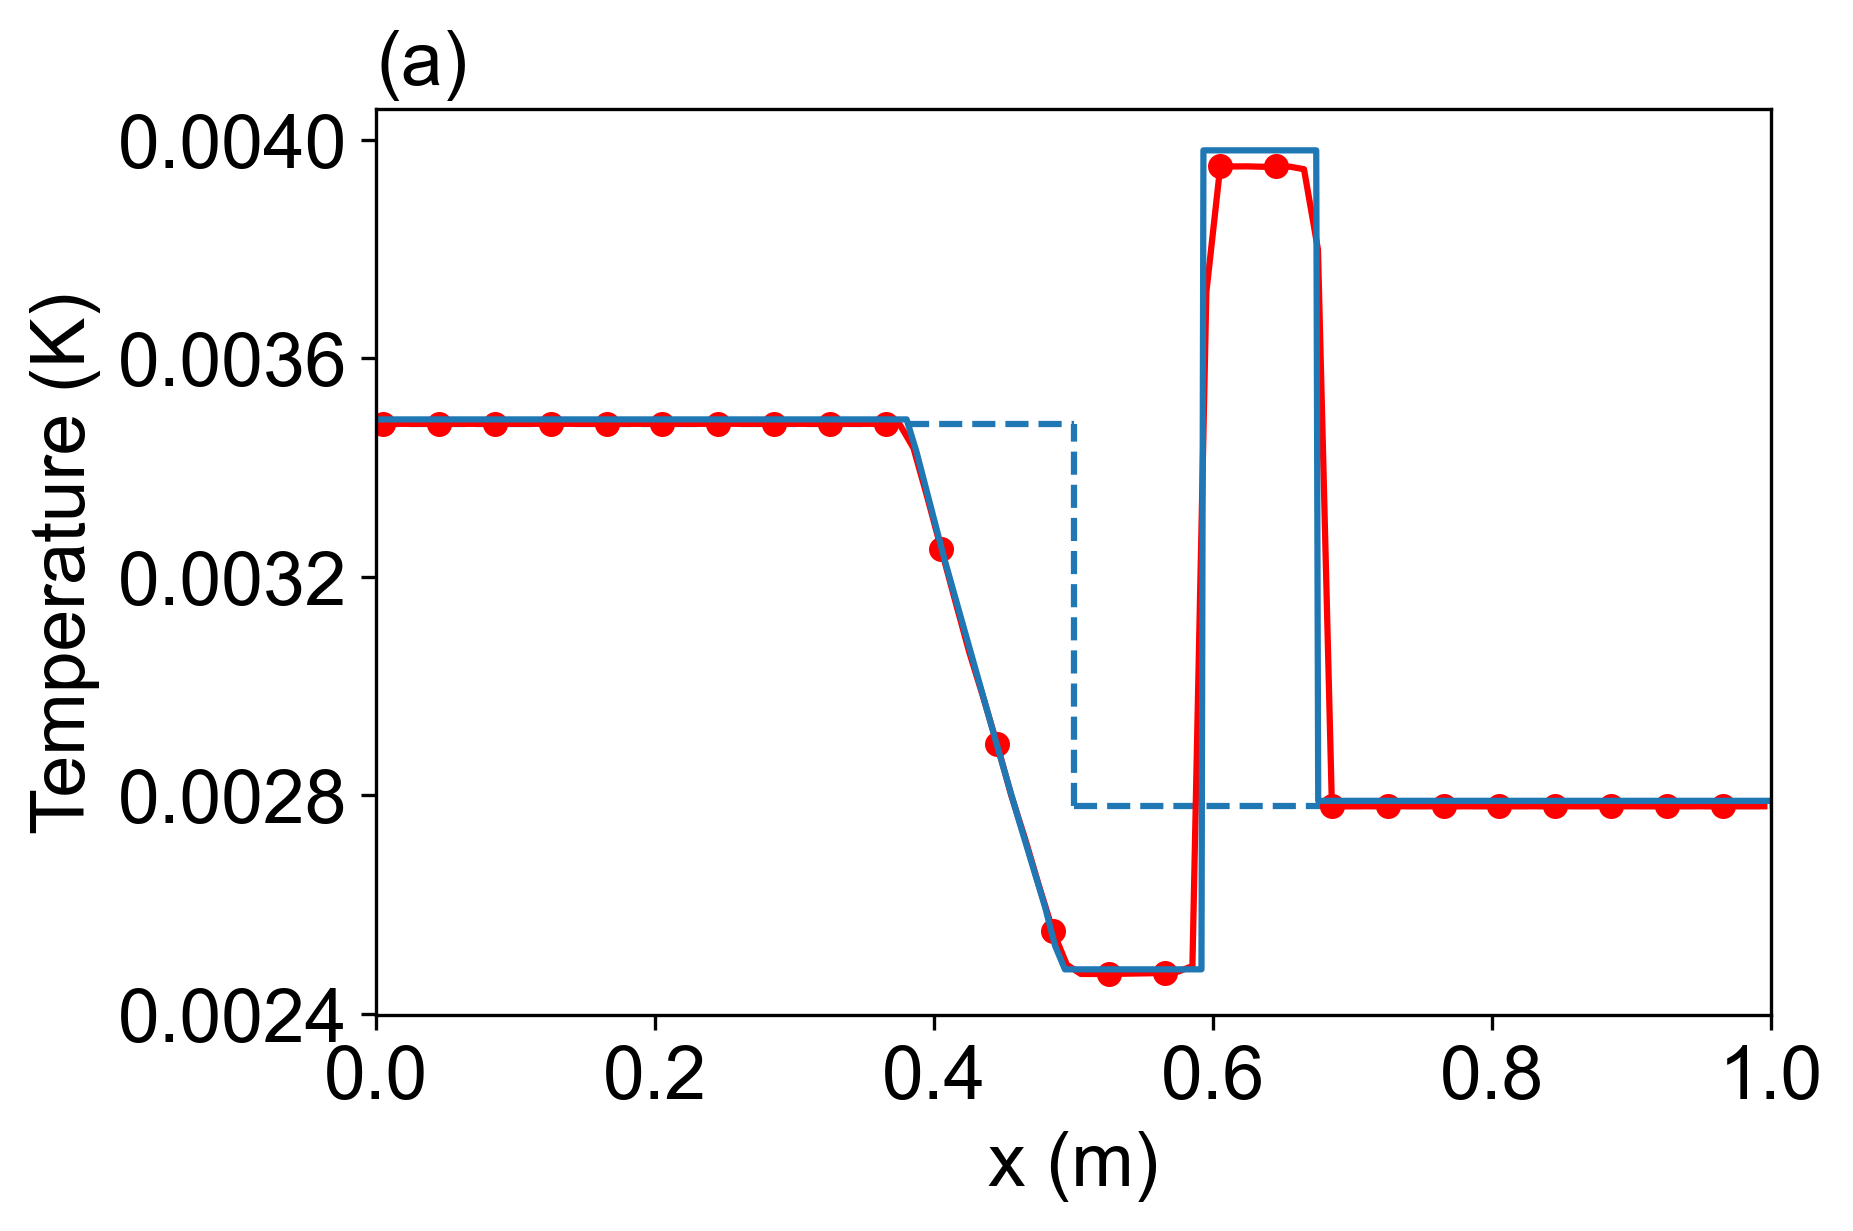
\includegraphics[width=0.465\linewidth]{sodT_v2.png}
            \includegraphics[width=0.435\linewidth]{sodP_V2.png}

        \caption{Validation of the VLE-based CFD solver by Sod shock tube simulations. Initial conditions: $P_{\rm{left}} = 1$ Pa, $P_{\rm{right}} = 0.1$ Pa, $T_{\rm{left}} = 0.00348$ K, $T_{\rm{right}} = 0.00278$ K, the initial discontinuity is at $x=0.5$ m; fluid: air; $t=0.1$ s; 200 grid cells, CFL = 0.2.}
        \label{vali1ST}
    \end{figure}
    
    
     \begin{figure}[htbp]

        \centering

            \includegraphics[width=0.45\linewidth]{valiT_v2.png}
            \includegraphics[width=0.45\linewidth]{valiP_v2.png}
        \caption{Verification of the VLE-based CFD solver by Chiapolino et al.'s shock tube simulations ~\cite{chiapolino2017simple}. Initial condition: $P_{\rm{left}} = 2$ bar, $P_{\rm{right}} = 1$ bar, $T_{\rm{left}} = 354$ K, $T_{\rm{right}} = 337$ K, $Y_{\rm{H_2O,\ left}} = Y_{\rm{H_2O,\ left}} = 0.3$, $Y_{\rm{Air,\ left}} = Y_{\rm{Air,\ left}} = 0.7$; $t = 1.0$ ms, 200 grid cells, CFL = 0.1, the initial discontinuity is at $x=0.5$ m.}
        \label{vali2ST}
    \end{figure}

    LES of a jet-in-crossflow is also conducted to validate the CFD solver. The results are compared with Su and Mungal's experimental data \cite{su2004simultaneous}. The experiments were performed in an updraft wind tunnel with air as the crossflow fluid and nitrogen as the jet fluid. The crossflow and nitrogen are both at 300 K and 1 atm. Nitrogen is seeded with acetone vapor to 10\% by volume for diagnostic purposes, which is also considered in the simulation. The tunnel crossflow velocity profile has a peak value of $v_{\infty}=2.95\ \rm{m/s}$. Nitrogen is injected from a nozzle with inner diameter $d=4.53\ \rm{mm}$, the jet average velocity is $u_0=16.9\ \rm{m/s}$. The mesh in the simulation contains 1.3M cells in total, and the average cell size is 2.3 mm. A finer mesh ($500\ \rm{\mu m}$) is used to capture the detailed flow structure near the injection nozzle. Based on the binary diffusivity of acetone and air ($D=0.104\ \rm{cm}^2\rm{s}^{-1}$) and the kinematic viscosity of air ($\nu=0.155\ \rm{cm}^2\rm{s}^{-1}$), Schmidt number, $Sc\equiv \nu/D$, of the system is 1.49. In Fig.~\ref{valiJIC}, the center streamline and \ce{N2} centerline of time-averaged field are compared between the simulation and experiments. The center streamline is the streamline that goes through the center of injector, and the \ce{N2} centerline is the line of maximum \ce{N2} concentration points at fixed-y planes. Length scales are properly normalized by the factor $rd$, where $d$ is the jet diameter (4.53 mm), $r$ is ratio of jet velocity to crossflow velocity: $r\equiv u_0/v_{\infty}=5.7$. The simulation results agree well with the experimental data at $x>2rd$, but show a small deviation near the injection nozzle.
    This validation indicates that our CFD solver and LES models can accurately predict the mixing process at least for ideal gas.

    \begin{figure}[htb]
        \begin{center}
            \includegraphics[width=0.5\linewidth]{valiJIC.png}
        \end{center}
        \caption{Comparison of a jet-in-crossflow between the present model prediction and experimental data~\cite{su2004simultaneous}. Blue: experimental data; red: simulation prediction.}
        \label{valiJIC}
    \end{figure}


\section{Influence of different diluents on mixture phase diagrams} \label{app:trad}
A key difference between the traditional gas turbine combustors and \ce{sCO2} oxy-combustors is their different diluents: the former one has \ce{N2} as its diluent, and the latter one has \ce{CO2} as its diluent. When the removal of \ce{N2} is incomplete, the \ce{sCO2} oxy-combustor can also have a mixture of \ce{N2} and \ce{CO2} as its diluent.

    \begin{figure}[htb]
        \centering

        \subfigure{
            \begin{minipage}[t]{1\linewidth}
                \centering
                \includegraphics[width=0.45\linewidth]{phase_diagram_PT_CH4_O2_N2.png}
                \includegraphics[width=0.45\linewidth]{phase_diagram_PT_CO2_CH4_O2_N2.png}
                %\caption{fig1}
            \end{minipage}%
        }%

        \subfigure{
            \begin{minipage}[t]{1\linewidth}
                \centering
                \includegraphics[width=0.45\linewidth]{RetrogradeCondensation.png}
                %\caption{fig2}
            \end{minipage}%
        }%

        \caption{Pressure-temperature phase boundaries and critical points of different mixtures: (a) \ce{CH4}/\ce{O2}/\ce{N2}, in which \ce{O2}:\ce{N2}=1:4 (which is close to the air composition); (b) \ce{CO2}/\ce{CH4}/\ce{O2}(/\ce{N2}), in which \ce{O2}:\ce{CH4}(:\ce{N2})=1:1(:4); (c) \ce{CO2}/\ce{CH4}/\ce{O2}, in which \ce{O2}:\ce{CH4}=1:1. Note the retrograde condensation behavior from A to B to C.}
        \label{v4}
    \end{figure}

Figure~\ref{v4}(a) shows the thermodynamic states of \ce{CH4}/\ce{O2}/\ce{N2} mixtures. Close to pure air or pure fuel, the critical pressure is relatively low. The highest mixture critical pressure is reached %by the fuel/air mixture 
at $z_{CH_4}=0.6$. Also, note that even for the range of $z_{CH_4}<0.6$, the trend of the mixture critical point is not monotonic (see the zoom-in figure), indicating that the real-fluid multiphase thermodynamics is highly nonlinear and any linear interpolation of mixture critical points is invalid. For all possible mixtures, the subcritical two-phase zone can only exist when the temperature is lower than 200 K. %Therefore, the mixtures in traditional gas turbine combustors must be in either the subcritical gas or supercritical gas-like phases.

Figure~\ref{v4}(b) shows the thermodynamic states of \ce{CH4}/\ce{CO2}/\ce{O2} mixtures with or without \ce{N2}. When $z_{CO_2}\geq0.6$, the influence of \ce{N2} addition is very small; but when $z_{CO_2}\leq0.5$, \ce{N2} addition can significantly increase the mixture critical pressure. By comparing Fig.~\ref{v4}(b) to Fig.~\ref{v4}(a), it is observed that \ce{CO2} addition can significantly increase the mixture critical pressure. However, at typical operating conditions of \ce{sCO2} oxy-combustion (100-400 bar and $\ge300$ K), the mixtures are still in supercritical gas-like or subcritical gas states, because the subcritical two-phase zone exists only when the temperature is lower than 300 K.

As shown by Fig.~\ref{v4}(c), retrograde condensation behavior can also occur in the \ce{CO2}/\ce{CH4}/\ce{O2} systems, similar as the \ce{CO2}/\ce{H2O} systems in Fig.~\ref{v3}.
%: when the gas (at point A) is compressed into the subcritical two-phase zone, phase separation can occur, and the gas partially condenses into liquid (at point B), but further compression makes the mixture go beyond the point of condensation with the effect that the liquid (at point B) evaporates again (i.e., the so-called ``retrograde condensation") to point C.% Similar but the reverse process occurs during the expansion. 

% \section{Compressibility and compressibility factor} \label{app:compressibility}
    
% Figure~\ref{fig:compressibility}(a) shows the mixture compressibility factor ($Z_{mix}=p/(\rho R T)$, describing how much the fluid behaves like ideal gas for which $Z_{mix}=1$) contour for the mixture of \ce{CO2}/\ce{H2O} with a feed of 0.3/0.7 (which is close to the product compositions of \ce{CH4} combustion). As expected, the subcritical liquid-phase zone (where the critical point of \ce{CO2} resides in) deviate most from ideal gas. For both subcritical two-phase zone and subcritical gas-phase zone, increased pressure push the mixture away from ideal gas, but increased temperature push the mixture towards ideal gas.
%     %The compressibility factor, $Z$, describes how much the fluid behaves like ideal gas. It is known that the compressibility factor of ideal gas is unity, and ideal gas is also considered to be easy to compress. In contrast, the liquid and solid with the compressibility factors much lower than unity behave very differently from the ideal gas, and both are considered as ``incompressible". Hence, low compressibility factor also represents low compressibility.

%     \begin{figure}[htb]
%         \centering
%         \subfigure{
%         %\begin{minipage}[t]{0.5\linewidth}
%             \centering
%             \includegraphics[width=0.45\linewidth]{compressibility_PT_CO2_H2O.png}
%         %\caption{fig2}
%         %\end{minipage}%
%         }%
%         \subfigure{
%             %\begin{minipage}[t]{0.5\linewidth}
%             \centering
%             \includegraphics[width=0.45\linewidth]{compress_rebut5cut.png}
%             %\caption{fig2}
%             %\end{minipage}%
%         }
%         \caption{(a) compressibility factor $Z_{mix}$ and (b) compressibility $\kappa$ of \ce{CO2}/\ce{H2O} mixture with a feed of 0.3/0.7.}
%         \label{fig:compressibility}

%     \end{figure}
    
% Strictly speaking, compressibility factor is not a measure of compressibility. Figure~\ref{fig:compressibility}(b) shows the isothermal compressibility ($\kappa=-\frac{1}{V}\big(\frac{dV}{dp}\big)_T$) contour for the same mixture. The subcritical liquid-phase zone has the lowest compressibility, which is even lower than that of the supercritical liquid-like zone. %It is found that the compressibility of this mixture is low, %and the required compression work are still very low, to maintain high thermal efficiency when the condition is close to the critical point of \ce{CO2}. However, it is due to the subcritical liquid state instead of the supercritical liquid-like state (i.e., ``dense fluid"). 
% In both subcritical two-phase zone and subcritical gas-phase zone, the compressibility is reversely proportional to pressure, but insensitive to temperature.
% %If the mixture is in the supercritical gas-like state (e.g., by pressures higher than 500 bar and temperatures higher than 600 K), then the compressibility is larger. %, and the system may need to lose more compression work in the compressor~\citep{ahn2015review,invernizzi2017prospects}.
\comment{
    \section{Grid convergence test of jet-in-crossflow LES} \label{app:coverge}

    To test the grid convergence, two more meshes are created for comparison. Compared with the original mesh in Fig.~\ref{JICFg}, one mesh (denoted as the Mesh 1) contains half as many cells by evenly coarsening the original mesh in three directions (i.e., cells length scale $\sim \sqrt[3]{2}$ original cells length scale), and the other mesh (denoted as the Mesh 2) contains one-fourth of cells by evenly coarsening the original mesh (i.e., cells length scale $\sim \sqrt[3]{4}$ original cells length scale). The same jet-in-crossflow case as in Sec.~\ref{sec:results:combustor:HPn} (the \ce{CO2}/\ce{H2O} mixture is 700 K, and has 20\% \ce{H2O} by mole; \ce{O2} (300 K) is injected.) is simulated using the new meshes. After the results reach the statistically stationary state, the mean gas mole fraction and mean density averaged over 1 ms (physical time) are shown in Fig.~\ref{converge}. %All three meshes provide similar predictions in the qualitative sense, but the penetration length prediction contains small perturbation.
    To better quantify the difference between the three results, the relative differences based on $L^2$ norm are computed (relative difference of property $v$ is defined as $\left\|v-v_{orig}\right\|_{L^2}/\left\|v_{orig}\right\|_{L^2}$) and shown in Table~\ref{converge:error}. Since the results at the fields far from the injection nozzle are similar, the relative difference computation only uses the data near the nozzle (i.e., the dashed box in Fig.~\ref{converge} (in the top left sub-figure)). As seen, refining the grid by a factor of two almost does not change the relative difference, and the relative differences are stably maintained at $\sim$0.2\%, $\sim$5\% and $\sim$5\% for gas mole fraction, density, and temperature, respectively. Hence, in terms of the relative differences between grids shown in Table~\ref{converge:error}, the original grid resolution in this work is sufficient.
    %In Fig.~\ref{converge}, penetration length prediction still fluctuates, which indicates that the grid is not perfectly converged. The VLE thermal model is computationally expensive and its SGS model for LES does not exist. Therefore, with the state-of-the-art, a perfect grid convergence probably cannot be achieved until a direct numerical simulation (DNS)-level grid (which can resolve Kolmogorov scales or smaller) is used, which is infeasible with limited computational resource. But for a qualitative research, and in terms of the relative difference between grids shown in Table~\ref{converge:error}, the original grid resolution in this work is sufficient.

    \begin{figure}[htbp]
        \centering
        %\subfigure{
            %\begin{minipage}[t]{0.5\linewidth}
        %    \centering
        %    \includegraphics[width=0.370\linewidth]{resub2_vf025_v2_cut_box.png}
        %    \includegraphics[width=0.320\linewidth]{resub2_vf05_v2_cut.png}
        %    \includegraphics[width=0.320\linewidth]{resub2_vf1_v2_cut.png}
            %\caption{fig1}
            %\end{minipage}%
        %}%

        %\subfigure{
            %\begin{minipage}[t]{0.5\linewidth}
        %    \centering
        %    \includegraphics[width=0.370\linewidth]{resub2_rho025_v2_cut.png}
        %    \includegraphics[width=0.320\linewidth]{resub2_rho05_v2_cut.png}
        %    \includegraphics[width=0.320\linewidth]{resub2_rho1_v2_cut.png}
            %\caption{fig2}
            %\end{minipage}%
        %}%

        %\subfigure{
            %\begin{minipage}[t]{0.5\linewidth}
        %    \centering
        %    \includegraphics[width=0.37\linewidth]{resub2_T025_v2_cut.png}
        %    \includegraphics[width=0.32\linewidth]{resub2_T05_v2_cut.png}
        %    \includegraphics[width=0.32\linewidth]{resub2_T1_v2_cut.png}
            %\caption{fig2}
            %\end{minipage}%
        %}%
        \includegraphics[width=1.0\linewidth]{9fig_c.png}
        \caption{Grid convergence test (the \ce{CO2}/\ce{H2O} mixture is 700 K, and has 20\% \ce{H2O} by mole, \ce{O2} (300 K) is injected.). Top: mean gas mole fraction, middle: mean density, bottom: mean temperature; left: Mesh 2, middle: Mesh 1, right: the original mesh.}
        \label{converge}
    \end{figure}

    \begin{table}[htbp]
        %\begin{center}
        \centering
        \begin{minipage}{0.9\textwidth}
            \caption{Relative difference with respect to the original mesh (based on $L^2$ norm).} \label{converge:error}
            \begin{center}
                \begin{tabular}{@{}l|ll@{}} %\hline
                    \toprule
                                      & Mesh 1   & Mesh 2   \\ %\hline
                    \midrule
                    Gas mole fraction & 0.195\% & 0.256\% \\%\hline
                    Density           & 4.392\% & 7.149\% \\ %\hline
                    Temperature       & 3.325\% & 5.737\% \\
                    \bottomrule
                \end{tabular}

            \end{center}
        \end{minipage}
        %\end{center}

    \end{table}

}



    %%=============================================%%
    %% For submissions to Nature Portfolio Journals %%
    %% please use the heading ``Extended Data''.   %%
    %%=============================================%%

    %%=============================================================%%
    %% Sample for another appendix section			       %%
    %%=============================================================%%

    %% \section{Example of another appendix section}\label{secA2}%
    %% Appendices may be used for helpful, supporting or essential material that would otherwise 
    %% clutter, break up or be distracting to the text. Appendices can consist of sections, figures, 
    %% tables and equations etc.



\begin{itemize}

%\item Chapter 1 introduces the analytic goals pursued in this thesis.

\item Chapter 2 briefly presents the history of, and science behind, the
subjects presented in this thesis.

\item In Chapter 3 the experiment is outlined.

\item Chapter 4 describes the simulation process used in the analysis.

\item Chapter 5 follows the chain of reconstruction software used to obtain
meaningful results from data.

\item Chapter 6 hashes out the strategy for analysis and presents the data and
simulated sets that will be used in the analysis.

\item Chapter 7 demonstrates the implementation of the event selection
processes.

\item In Chapter 8 those events selected in Chapter 7 are analyzed.

\item Chapter 9 presents a final discussion of the analyses presented in the
thesis.

\end{itemize}
%%%%%%%%%%%%%%%%%%%%%%%%%%%%%%%%%%%%%%%%%%%%%%%%%%%%%%%%%%%%%%%%%%%%%%%%%%%%%%%%
